\documentclass{report}
\usepackage{longtable}
\usepackage{adjustbox}
\usepackage[intlimits]{amsmath}
\usepackage{mathtools}
\usepackage{nonfloat}
\usepackage{amsmath}
\usepackage{verbatim}
\usepackage{amsthm}
\usepackage{setspace}
\usepackage[paperwidth=16cm,paperheight=24cm]{geometry}
\usepackage[a4,frame,center]{crop}
%\graphicspath{{/home/abhishek/Desktop/"Text Classification"/Report/figures/}}
\graphicspath{{./figures/}}
\usepackage{lipsum}% dummy text
\usepackage[titles]{tocloft}
\usepackage{amssymb}
\setlength\cftbeforechapskip{100pt}
\renewcommand\cftfigafterpnum{\vskip10pt\par}
\renewcommand\cfttabafterpnum{\vskip10pt\par}
%\usepackage[superscript,biblabel]{cite}
\usepackage[superscript]{cite}

\usepackage{tocloft,lipsum,pgffor,sectsty}
\setcounter{tocdepth}{4}% Include up to \subsubsection in ToC

\sectionfont{\huge}
\subsectionfont{\LARGE}
\subsubsectionfont{\Large}
\paragraphfont{\large}



% Font changes to ToC content of sectional units
\renewcommand{\cftpartfont}{\normalfont\sffamily\bfseries}% \part font in ToC
\renewcommand{\cftchapfont}{\normalfont\large\itshape}    % \chapter font in ToC
\renewcommand{\cftsecfont}{\normalfont\slshape}           % \section font in ToC
\renewcommand{\cftsubsecfont}{\normalfont\itshape}        % \subsection font in ToC
\renewcommand{\cftsubsubsecfont}{\normalfont\small}       % \subsubsection font in ToC

% Font changes to document content of sectional units
\renewcommand{\partfont}{\normalfont\HUGE\bfseries}
\renewcommand{\chapterfont}{\normalfont\HUGE\bfseries}
\renewcommand{\sectionfont}{\normalfont\Huge\bfseries}
\renewcommand{\subsectionfont}{\normalfont\Huge\bfseries}

\usepackage{url}
\usepackage{enumitem}
\usepackage{chngcntr}
\usepackage[svgnames]{xcolor}
\usepackage{pgfplotstable,booktabs}
\usepackage{csvsimple}
\usepackage{multicol}
\usepackage[pdfpagemode=FullScreen, colorlinks=true]{hyperref} 
\hypersetup{%
  colorlinks = false,
  linkcolor  = black
}
\usepackage{graphicx}
\usepackage{subcaption}
\usepackage{filecontents}
\newcommand{\plogo}{\fbox{$\mathcal{PL}$}}
\usepackage[utf8]{inputenc}
\usepackage[T1]{fontenc}
\usepackage{fouriernc}
\usepackage[utf8]{inputenc}
\usepackage{etoolbox}
%\makeatletter
%\patchcmd{\ttlh@hang}{\parindent\z@}{\parindent\z@\leavevmode}{}{}
%\patchcmd{\ttlh@hang}{\noindent}{}{}{}
%\makeatother
\usepackage{titletoc}
\usepackage[figurename=Fig - ]{caption}
\captionsetup[table]{skip=20pt}
\captionsetup[figure]{skip=20pt}
\usepackage[tablename=Table - ]{caption}
\setcounter{secnumdepth}{4}

\usepackage{setspace}
%FOR ADDING numbering in chapter, sections etc.
\usepackage{titlesec}
\titleformat{\chapter}[display]
  {\normalfont\Huge\bfseries}{}{0pt}{\Huge\ifnum\value{chapter}>0\relax\arabic{chapter}.~\fi\ \ }
 \titleformat{\section}[display]
  {\normalfont\Huge\bfseries}{}{0pt}{\LARGE\thechapter.\ifnum\value{section}>0\relax\arabic{section}.~\fi\quad}
  \titleformat{\subsection}[display]
  {\normalfont\Huge\bfseries}{}{0pt}{\Large\thesection.\ifnum\value{subsection}>0\relax\arabic{subsection}.~\fi\quad}
  \titleformat{\subsubsection}[display]
  {\normalfont\Huge\bfseries}{}{0pt}{\large\thesubsection.\ifnum\value{subsubsection}>0\relax\arabic{subsubsection}.~\fi\quad}



\titlespacing{\chapter}{0cm}{0pt}{10pt}
\titlespacing{\section}{0cm}{0pt}{0.2cm}
\titlespacing{\subsection}{0cm}{0pt}{0.2cm}
\titlespacing{\subsubsection}{0cm}{0pt}{0.2cm}


\usepackage{geometry}
 \geometry{
 a4paper,
 tmargin=20mm,
 bmargin=15mm,
 left=20mm,
 right=20mm,
 top=20mm,
 }

%\renewcommand\thesection{\arabic{section}}
\titlecontents{chapter}[1.05em]{\bigskip}%
{\contentslabel[\MakeUppercase{\thecontentslabel}]{1em}\enspace\textsc}%numbered\contentslabel
{\hspace*{-1em}\textsc}%numberless
{\hfill\contentspage}%
%
%\titlecontents{section}[1.6em]{\bigskip}%
%{\thecontentslabel.\enspace}%numbered
%{}%numberless
%{\titlerule*[1pc]{.}\contentspage}%

\setcounter{tocdepth}{6}

\usepackage{lipsum}

\newcommand\myfigure[1]{%
\medskip\noindent\begin{minipage}{\columnwidth}
\centering%
#1%
%figure,caption, and label go here
\end{minipage}\medskip}




\newenvironment{changemargin}[1]{%
\item[]}{\end{list}}
\setlength{\columnsep}{0cm}


%\titlespacing*{\chapter}{0pt}{0pt}{20pt}

\renewcommand{\bibname}{References}

\usepackage{makeidx}
\makeindex

\begin{document} 

\begin{titlepage}
	\centering
	
\includegraphics[width=4cm]{logo.png}\\[.5cm]
	{\scshape\LARGE Indian Institute of \\Information Technology, Allahabad \par}
	\vspace{1cm}
	\rule{\textwidth}{2pt}	
	%\vspace{2pt}\vspace{-\baselineskip}
	%\rule{\textwidth}{0.4pt}
	\vspace{0.15\textheight}
		
	\textcolor{Red}{ 
		{\fontsize{35}{52}\selectfont Social Delivery : \\[8pt] An Android Application}\\[0.5\baselineskip]
	}
	
	\vspace{0.15\textheight} 
	\setlength\columnsep{0pt}
	\rule{0.3\textwidth}{0.4pt} 
	\begin{multicols}{3} 
	\textcolor{Blue}{
		\begin{flushleft} 
		{\large \quad \quad \quad \quad Ayush Agnihotri}\\[8pt] 
		{\large \quad \quad \quad \quad Nidheesh Pandey}\\[8pt]
		{\large \quad \quad \quad \quad Abhishek Pasi}\\[8pt]
		\end{flushleft}
		}
		\columnbreak
		 
	\textcolor{Blue}{
		\begin{flushleft} 
		{\large IIM2015004}\\[8pt] 
		{\large IIM2015501}\\[8pt]
		{\large ICM2015002}\\[8pt]
		\end{flushleft}
		}
		\columnbreak

	\textcolor{Green}{
		\begin{flushright}
		{\Large \textsc{Under supervision}}\\[8pt]
		{\large of}\\[8pt]
		{\Large \textsc{\textbf{Dr. Jagpreet Singh}}}\\[8pt]
		\end{flushright}
		}
	\end{multicols}
	\vspace{0.015\textheight} 
	
\hfill


	\rule{\textwidth}{0.4pt} % Thin horizontal rule
	
	\vspace{2pt}\vspace{-\baselineskip} % Whitespace between rules
	
	\rule{\textwidth}{2pt} % Thick horizontal rule
	
\end{titlepage}
\pagebreak

%---------------------------------------------------------------------------------------------------

{\chapter*{ \quad \quad \quad \quad \quad \quad  \Huge \scshape \underline {Declaration} }
\vspace{2.0cm}
\begin{spacing}{0.3}
\fontsize{17}{68}\selectfont\linespread{10} {We hereby declare that the work presented in this project report entitled \textbf{``Social Delivery''},  submitted towards progress of summer project report of Dual Degree(IT) at \textbf{Indian Institute of Information Technology, Allahabad}, is an authenticated record of our original work carried out from \textbf{May 2018} to \textbf{present} under the guidance of \textbf{Dr. Jagpreet Singh}. Due acknowledgements have been made in the text to all other material used. The project was done in full compliance with the requirements and constraints of the prescribed curriculum.}
\end{spacing}
\vspace{3cm}
\Large
\noindent \textbf{Signature Of Supervisor:}\\
\rule[0.5em]{25em}{0.5pt} % This prints a line for the signature
\vspace{1cm}\\
\noindent \textbf{Date:}\\
\rule[0.5em]{25em}{0.5pt}\\ % This prints a line to write the date
\vspace{1cm}\\
\noindent \textbf{Signature Of Students:}\\
\rule[0.5em]{12em}{0.5pt} % This prints a line for the signature
\vspace{1.5cm}\\

}


%----------------------------------------------------------------------------------------
%---------s-------------------------------------------------------------------------------
%	LIST OF CONTENTS/FIGURES/TABLES PAGES
%----------------------------------------------------------------------------------------

\pagenumbering{arabic}
{ \doublespacing
\pagenumbering{roman}
\tableofcontents % Prints the main table of contents

\addtocontents{toc}{~\hfill\textbf{Page}\par}
\pagebreak
\listoffigures % Prints the list of figures
\pagebreak
%\listoftables % Prints the list of tables
%\pagebreak

}

%-----------------------------------------------------------------------------------------
\title{\fontsize{45}{66.6}\selectfont  Social Delivery\linebreak}
\date{}
\maketitle
\setlength{\columnsep}{0.7cm}
\pagenumbering{arabic}
%\begin{multicols}{1}

%---------------------------------------------------------------------

\chapter{Introduction and Motivation}
\bigskip
\bigskip
\par \Large Online Shopping is growing at a fast pace. People prefer shopping for products online rather than offline. However, when you need to buy things from local markets less options are available. Normally, people go to shops or send somebody to buy goods for them. They may also ask someone who is going to market to buy things for them.\\

We have tried to provide a solution to above problem by developing an android application. With this application we aim to automate the process of communication between potential deliverers and shoppers.\\


People go for shopping, at the same time their friends and other people may also want to buy things from same or nearby markets. These people going for shopping can help their friends. They will also get some incentive in terms of delivery charge without much effort.\\

We aim to provide an efficient way to manage the shopping needs of people from local markets. Any user using our app is free to use it as a shopper or deliverer. Sometimes you can be a shopper and at other times you can be a deliverer. Shoppers are driven by their shopping needs and deliverers are motivated to use our app for incentive they get in return of their service.\\  

We named this application as `\textbf{Social Delivery}', Since,  it creates a social shopping environment . \\


%---------------------------------------------------------------------------------------------------

\chapter{Related work}
\bigskip
\bigskip
\par As you already know,  we have made an android application which helps people shop from local shops, it will be helpful to discuss what work has been already done in this space.\\

\par Let\textquotesingle s have a look at the local shopping market space. While amazon is leader in online shopping and e-commerce, it has also entered into grocery delivering area. Ever heard of Google selling groceries and small daily use items? Yes it is true, Google which is one of the biggest technology company has also entered into this space with its
\textbf{Google express\cite{c7}}. From what we have seen it has partnered  with various big store chains like walmart and offers free delivery over a certain cost. Although, it is not available in India as of now.\\

\par Taxi booking apps are also taking a step in local delivery space. Uber experimented with \textbf{UberFresh\cite{c1}} in the past (2014). Now it has successfully launched \textbf{UberEats\cite{c3}}, which serves worldwide.  It aims to deliver fast food from local restaurant chains in about 10 minutes or less. We already know Zomato, Swiggy and Foodpanda are working in this area, but taxi services entering in this area is totally a new thing. Ola has acquired foodpanda and aims to do the same things as UberEats.\\
Gett is another taxi app which brings items from shops and restaurants , it has joined hands with WunWun , a delivery app to facilitate the same. It delivers every product you can buy from a local shop. \\

\par Taxi companies are competing with big players like amazon and google . Although google is new in this space , being a tech giant , it has plenty of resources. Apart from that they have are giving major competition to delivery startups like Postmates\cite{c10} , DoorDash\cite{c5} and Instacart\cite{c4}. We will talk about these startups in brief.\\

An important point to note is, these type of local delivery services are currently not available in India. However, food delivery services like zomato , swiggy and foodpanda are quite popular.\\
Now coming to services which have quite a resemblance with our application.
Local delivery startups like Instacart\cite{c4}, DoorDash\cite{c5} and  Postmates are getting quite popular in the US.\\

Postmates works with both stores and restaurants to provide services to its customers. Currently it serves 14 cities across the US. An order placed by a user ,  is purchased and delivered by a local courier which they call “hipster on wheels” . It closely resembles what we have implemented in our android application. \\

Instacart\cite{c4}, it focuses more on grocery shopping. It sends a local shopper to a grocery store you wanted to shop from, goods are delivered within an hour.\\

DoorDash\cite{c5} helps in doing local delivery from restaurants . It takes about 45 minutes and serves areas in Silicon Valley , Los Angeles , Boston and Chicago.\\

Our application is quite simple and works on more or less on the same concepts described in this section. However, there are some key differences in our design and working style of application.\\

%------------------------------------------------------------------------------------------------------------------

\chapter{Software Requirement Specification}
\section{Introduction}
\subsection{Purpose}
The purpose of this report is to describe and examine all assorted ideas that have come up to define our application and to give a detailed description of software requirements and technologies used to develop our application “Social Delivery”. It also describes its user interface and specifies all its functional and non-functional requirements as well as design constraints. Various use-cases are discussed and Use-case diagrams are also used to explain the structure of the application and provide all actions performed by various actors.

\subsection{Scope}
Our “\textbf{Social Delivery}” application will help people around the world who are using our app as Shoppers to order market products from their homes and get them delivered at their doorstep for a small delivery charge. Deliveries will be made by other users who are using the app as Deliverers.
The users using our app as shoppers will benefit as they are getting their delivery to wherever they want without going anywhere themselves .The users who are using our app as deliverers will also benefit as they will get paid for the delivery in the form of delivery charge.
In this way both the parties involved are happy.

\subsection{Overview}
The next section, \textbf{Overall Description}, of this document gives an overview of the functionalities of our application. It describes the informal requirements and is used to establish a context for the technical requirements specification in the next section. 

The third section, \textbf{Requirements}, of this document is written primarily for the developers and describes in technical terms the details of the functionality of the product. 
Both sections of the document describe the same software product in its entirety, but are intended for different audiences and thus use different language.


\section{Overall Description}
\subsection{Product perspective}

\begin{itemize}[label=$\circ$]
\item This app is an Android based application designed on \textbf{Android Studio} platform.
\item It uses \textbf{Google Firebase\cite{c9}} Database which is a NoSQL Real-time cloud-hosted Database. We store the profiles of all users and all the data of the orders placed by them in a JSON tree. 
\item It uses \textbf{Google Places API} to set the delivery location of an order and \textbf{Google maps\cite{c2}} to help the Deliverers to reach the delivery location by showing them the path. 
\item Our app also uses \textbf{GPS Location} to find the current city of the user. 
\item Notification alerts are also sent to users on every status change of their orders using the \textbf{One Signal API\cite{c16}}. The One Signal API  is an open source service which uses \textbf{Google Cloud Messaging(GCM)\cite{c11}} in its backend.
\end{itemize}

\subsection{Product features}

For Users using our app as Shopper :
\begin{itemize}[label=$\circ$]
\item Place a new order.
\item Edit existing pending orders.
\item Filter the orders according to status like All, Active, Pending, Finished, Cancelled, Expired.
\item See his/her PayTM wallet balance.
\item Check the details of the deliverer who have accepted his/her order.
\item Switch to deliverer view.
\item Sign-out from the app.
\end{itemize}

For Users using our app as Deliverer:
\begin{itemize}[label=$\diamond$]
\item Accept a pending order out of a list of all pending orders from his city location.
\item Reject an accepted order.
\item See the path to reach the delivery location for an order.
\item See his/her current location(city).
\item Filter the orders according to status like All, Active, Pending, Finished, Cancelled, Expired.
\item See his/her PayTM wallet balance.
\item Complete the delivery of an accepted order by OTP verification. 
\item Switch to shopper view.
\item Sign-out from the app.
\end{itemize}

\subsection{User characteristics}
\begin{itemize}
\item The user must have a smartphone with Android OS and must know how to operate basic android apps.
\end{itemize}

For Users using our app as Shopper:
\begin{itemize}[label=$\diamond$]
\item The user must know how to use pick places from a google maps.
\item The description of the orders should be as clear as possible.
\item The estimated price range of order should be given as close as possible to the real price.
\item Appropriate expiry Date \& Time of the order should be given (if any).
\item Delivery location should be set appropriately. 
\item The user must know how to pay using PayTM wallet.
\end{itemize}

For Users using our app as Deliverer:
\begin{itemize}[label=$\diamond$]
\item The user should know how to use Google maps app.
\item The user must know how basic OTP verification process works.
\item Users using our app as Deliverers should choose wisely what orders they can deliver.
\end{itemize}

\subsection{Constraints}
\begin{itemize}
\item Active internet connection is required while using this app.
\item E-mail ID of the users should be valid.
\item GPS should be working properly.
\item Google maps application(optional) should be installed in the Android device to be able to use SHOW PATH functionality.
\item Database constraints:
\begin{itemize}
\item As we are using the free version of the Firebase, we are limited to a maximum of 100 active connections (users) simultaneously at a time.
\item Currently we can store a total of 1 GB data on our database.
\end{itemize}
\end{itemize}

\subsection{Assumptions and dependencies}

\begin{itemize}
\item The device which is used for our app should have Android OS version 6 or above. 
\item We are assuming that the PayTM payment service which we are using for payment of order will be available all the time and will work without any errors.
\item We are assuming the GPS location will always give correct results.
\item No more than one user who is using our app as Deliverer should Accept a single order at the same time.
\end{itemize}

\section{Requirements}

\subsection{Functional Requirements}

\noindent \newline
\textbf{Module-1 :} User Login using E-mail \& Password
\begin{description}
\item AIM : User can login to our app using unique E-mail \& Password
\item INPUT : E-mail and password.    
\item OUTPUT :  Displays a message if username and password does not match otherwise enter into the Usage mode screen.
\item PROCESS : Match username and password from database.
\end{description}

\noindent \newline \textbf{Module-2 :} User Login using Google Sign-in\cite{c15}
\begin{description}
\item AIM : User can login to our app using G-Mail ID.
\item INPUT : G-Mail ID (E-mail and password).
\item OUTPUT : enter into the Usage mode screen.
\item PROCESS : Use GoogleApiClient.
\end{description}

\noindent \newline \textbf{Module-3 :} Reset Password
\begin{description}
\item AIM : User can reset password using registered E-mail.
\item INPUT : Registered E-mail.
\item OUTPUT : Password reset link sent to registered E-mail.
\item PROCESS : Use Firebase Authentication functions.
\end{description}

\noindent \newline \textbf{Module-4 :} Registration
\begin{description}
\item AIM : A new user can register to our app by filling the form.
\item INPUT : Name, Mobile No., Alternate Mobile No.(optional), E-mail and password.
\item OUTPUT : E-mail verification link sent to given E-mail if E-mail valid otherwise asks to enter valid E-mail address.
\item PROCESS : Use Firebase Authentication functions.
\end{description}

\noindent \newline \textbf{Module-5 :} Verify E-mail
\begin{description}
\item AIM : User will follow the instructions given in link for E-mail verification to verify E-mail before using our app.
\item INPUT : Press Refresh Button.
\item OUTPUT : Enter into the Usage mode screen if E-mail verification successful else remain in E-mail verification screen.
\item PROCESS : Save all data in database.
\end{description}

\noindent \newline \textbf{Module-6 :} Re-send Verification E-mail
\begin{description}
\item AIM : Re-send the E-mail verification link to entered E-mail while registering.
\item INPUT : Touch Re-send Verification Mail button.
\item OUTPUT : Verification E-mail sent to E-mail.
\item PROCESS : Use Firebase Authentication functions.
\end{description}

\noindent \newline {\textbf{Module-7 :}} Place a new order
\begin{description}
\item AIM : User can place a new order when using our app as Shopper by filling a form.
\item INPUT : Description or order, Category, Estimated price range minimum and maximum values, Expiry Date and Time of order(optional) and delivery location.
\item OUTPUT : PayTM payment gateway if all details are valid else displays appropriate message.
\item PROCESS : Check maximum and minimum value and whether all mandatory fields are filled.
\end{description}

\noindent \newline \textbf{Module-8 :} Order payment
\begin{description}
\item AIM : Finish payment of the order by paying from PayTM wallet using PayTM payments SDK.
\item INPUT : PayTM login details.
\item OUTPUT : Order details added in Database and details updated in Database if payment successful else no change in database.
\item PROCESS : Save all data in database and send notification to shopper.
\end{description}


\noindent \newline \textbf{Module-9 :} Edit pending order
\begin{description}
\item AIM : User can edit an existing pending order when using our app as Shopper by filling a form.
\item INPUT : Description of order, Category, Estimated price range minimum value, Expiry Date and Time of order(optional) and delivery location.
\item OUTPUT : opens order view screen if all details are valid else displays appropriate message.
\item PROCESS : Save all data in database.
\end{description}

\noindent \newline \textbf{Module-10 :} Apply a filter
\begin{description}
\item AIM : Displays the orders according to selected filters.
\item INPUT : Touch the filter option that you want to apply in the Navigation drawer of Shopper or Deliverer view.
\item OUTPUT : Recycler view containing cards of orders of chosen status only.
\item PROCESS : Database query to fetch orders from database of chosen status.
\end{description}

\noindent \newline \textbf{Module-11 :} Sign-out
\begin{description}
\item AIM : To Sign-out of the app.
\item INPUT : Touch Sign Out button in the Navigation drawer\cite{c13} of Shopper or Deliverer view.
\item OUTPUT : Signs out of the app and displays the login screen.
\item PROCESS : Use Firebase Authentication functions.
\end{description}

\noindent \newline \textbf{Module-12 :} View as Deliverer
\begin{description}
\item AIM : Switch to Deliverer mode from the Shopper mode.
\item INPUT : Touch View as Deliverer button in the Navigation drawer of Shopper view.
\item OUTPUT : Opens the Deliverer view.
\item PROCESS : Call the intent for the Deliverer view.
\end{description}

\noindent \newline \textbf{Module-13 :} View as Shopper
\begin{description}
\item AIM : Switch to Shopper mode from the Deliverer mode.
\item INPUT : Touch View as Shopper button in the Navigation drawer of Deliverer view.
\item OUTPUT : Opens the Shopper view.
\item PROCESS : Call the intent for the Shopper view.
\end{description}

\noindent \newline \textbf{Module-14 :} Show Path
\begin{description}
\item AIM : Shows the path to delivery location of an order to the Deliverer using Google maps.
\item INPUT : touch Show Path button.
\item OUTPUT : Opens the path in Google maps.
\item PROCESS : Calls the Google maps app.
\end{description}

\noindent \newline \textbf{Module-15 :} Accept an order
\begin{description}
\item AIM : Accept a pending order.
\item INPUT : touch Accept button in Deliverer order detailed view.
\item OUTPUT : Enables Complete Order button.
\item PROCESS : Update details in database  and send notification to shopper.
\end{description}

\noindent \newline \textbf{Module-16 :} Reject an order
\begin{description}
\item AIM : Reject an accepted order.
\item INPUT : touch Reject button in Deliverer order detailed view.
\item OUTPUT : Disables Complete Order button.
\item PROCESS : Update details in database and send notification to shopper.
\end{description}

\noindent \newline \textbf{Module-17 :} Complete an order
\begin{description}
\item AIM : Complete the delivery of an accepted order.
\item INPUT : touch Complete Order button in Deliverer order detailed view.
\item OUTPUT : opens SENT OTP screen.
\item PROCESS : calls intent for SENT OTP screen.
\end{description}

\noindent \newline \textbf{Module-18 :} Send OTP
\begin{description}
\item AIM : Send OTP to the shopper from the deliverer.
\item INPUT : actual price of item bought.
\item OUTPUT : opens ENTER OTP screen.
\item PROCESS : Update details in database and send notification to shopper.
\end{description}

\noindent \newline \textbf{Module-19 :} Finish Order
\begin{description}
\item AIM : Finish the delivery of an order.
INPUT : OTP as received from shopper.
\item OUTPUT : Delivery finished if correct OTP entered otherwise displays message.
\item PROCESS : Update details in database and send notification to shopper.
\end{description}

\subsection{Non- functional Requirements}

\subsubsection{Performance Requirements}
The response time should be less and the actions taken by user should not take much time. The access to database should be fast enough. The amount of graphics/animations should be such that it ensure all the above points.

\subsubsection{Availability}
The application will run 24x7 if internet connection is available.

\subsubsection{Security}
The Database used to store all the application related data should be secure against any malicious activity.

\subsubsection{Reliability}
This application has been tested on Android Oreo, Android Marshmallow, custom UIs like MIUI (Xiaomi phones), EMUI (Honor phones) and will run on any android phone having Android SDK version 6 or above.

\subsubsection{Fault Tolerance}
The data stored in the database should not get corrupted by any means like system crash, power failure or lost internet connectivity. The information stored in database should be resistance to any unwanted changes.

\subsubsection{Portability}
The application should work on any android device like mobile phones, tablets, fablets etc.

\subsubsection{Maintainability}
It should be easy to add any new feature as per requirement anytime.

\subsection{External Interface Requirements}
\subsubsection{User Interfaces}

\begin{itemize}
\renewcommand{\labelitemi}{$\rightarrow$}
\item For Front-end : XML(eXtensible Markup Language) and Android(Java)
\item For Back-end : Google Firebase Database            
\end{itemize}

\subsubsection{Hardware Interfaces}
Any device with Android OS like mobile phone, tablet or fablet.

\subsubsection{Software Interfaces}
\begin{itemize}[label=$\diamond$]
\item Softwares :
\begin{itemize}[label=$\rightarrow$]
\item Android Studio : Development environment for Google\textquotesingle s Android operating system.
\end{itemize}
\item Languages :
\begin{itemize}[label=$\rightarrow$]
\item For Front-end : XML(eXtensible Markup Language) and Android(Java)
\item For Back-end : Java
\end{itemize}

\item Tools / Libraries:
\begin{itemize}[label=$\rightarrow$]
\item Google Sign-in
\item E-mail verification (using Firebase Authentication)
\item Google Places API
\item Google Maps
\item Location
\item PayTM payments SDK\cite{c17}
\item OneSignal API (for Notifications)
\item Lucidchart.com\cite{c12} (for diagrams)
\end{itemize}

\item Databases :
\begin{itemize}[label=$\rightarrow$]
\item Google Firebase (NoSQL Real-time cloud-hosted Database) :
\begin{enumerate}
\item Data is synced across all clients in realtime, and remains available when your app goes offline.
\item Data is stored as JSON (JavaScript Object Notation) tree.
\end{enumerate}
\end{itemize}

\end{itemize}

\subsubsection{Communications Interfaces}
Internet connection in the device through any medium like 3G, 4G or Wifi.

\subsection{Use-cases}
This application is mainly used for shopping for items from local stores.
\begin{itemize}
\item In our current design of application we have a community of shoppers and deliverers using our app.
\item Any user can choose to become a shopper or deliverer . Some days you can be a shopper and on other days you can be a deliverer.
\end{itemize}

\textbf{Use case 1 :  as a shopper.}\\
You want to buy some item from a shop but you are too busy to go there . You can simply use this application and someone will deliver the product at your doorstep. \\

\textbf{Use case 2 : as a shopper with some urgency.}\\
You want  some item before a certain time . Just put your deadline as expiry date . It is useful when you don’t want anyone to accept your order  after your deadline . 
It is also obvious that deliverers will process the order which has more incentive. We can have provision for tips also . Although , it is not included in current version of app.\\

\textbf{Use case 3: as a deliverer who is in market.}\\
You are currently in main market of your city and you are done with your shopping . You open our app and find many users want goods which are easily available in this market  . It’s an earning opportunity for you.\\

\textbf{Use case 4: as a deliverer with a will to earn.}\\
Today you have some free time .  You open the application and see many orders with a familiar destination and marketplace. You decide  it is a good opportunity to earn something . You accept some orders and process them to earn incentives (delivery charge).\\
The above four use cases clearly describe the utility of our application . However , with the same design and some changes we can easily convert this application to have more use cases.\\

Example of few such use cases :-
\begin{enumerate}[label=\alph*.]
\item Partnering with local shops and having centralised system of delivery between the shop and its customers. 
\item Having listing of shops and using the application to buy goods from shops.
\item Partnering with restaurants for booking tables or ordering food items from their menu.
\end{enumerate}

\section{Diagrams}
\begin{figure}[h!]
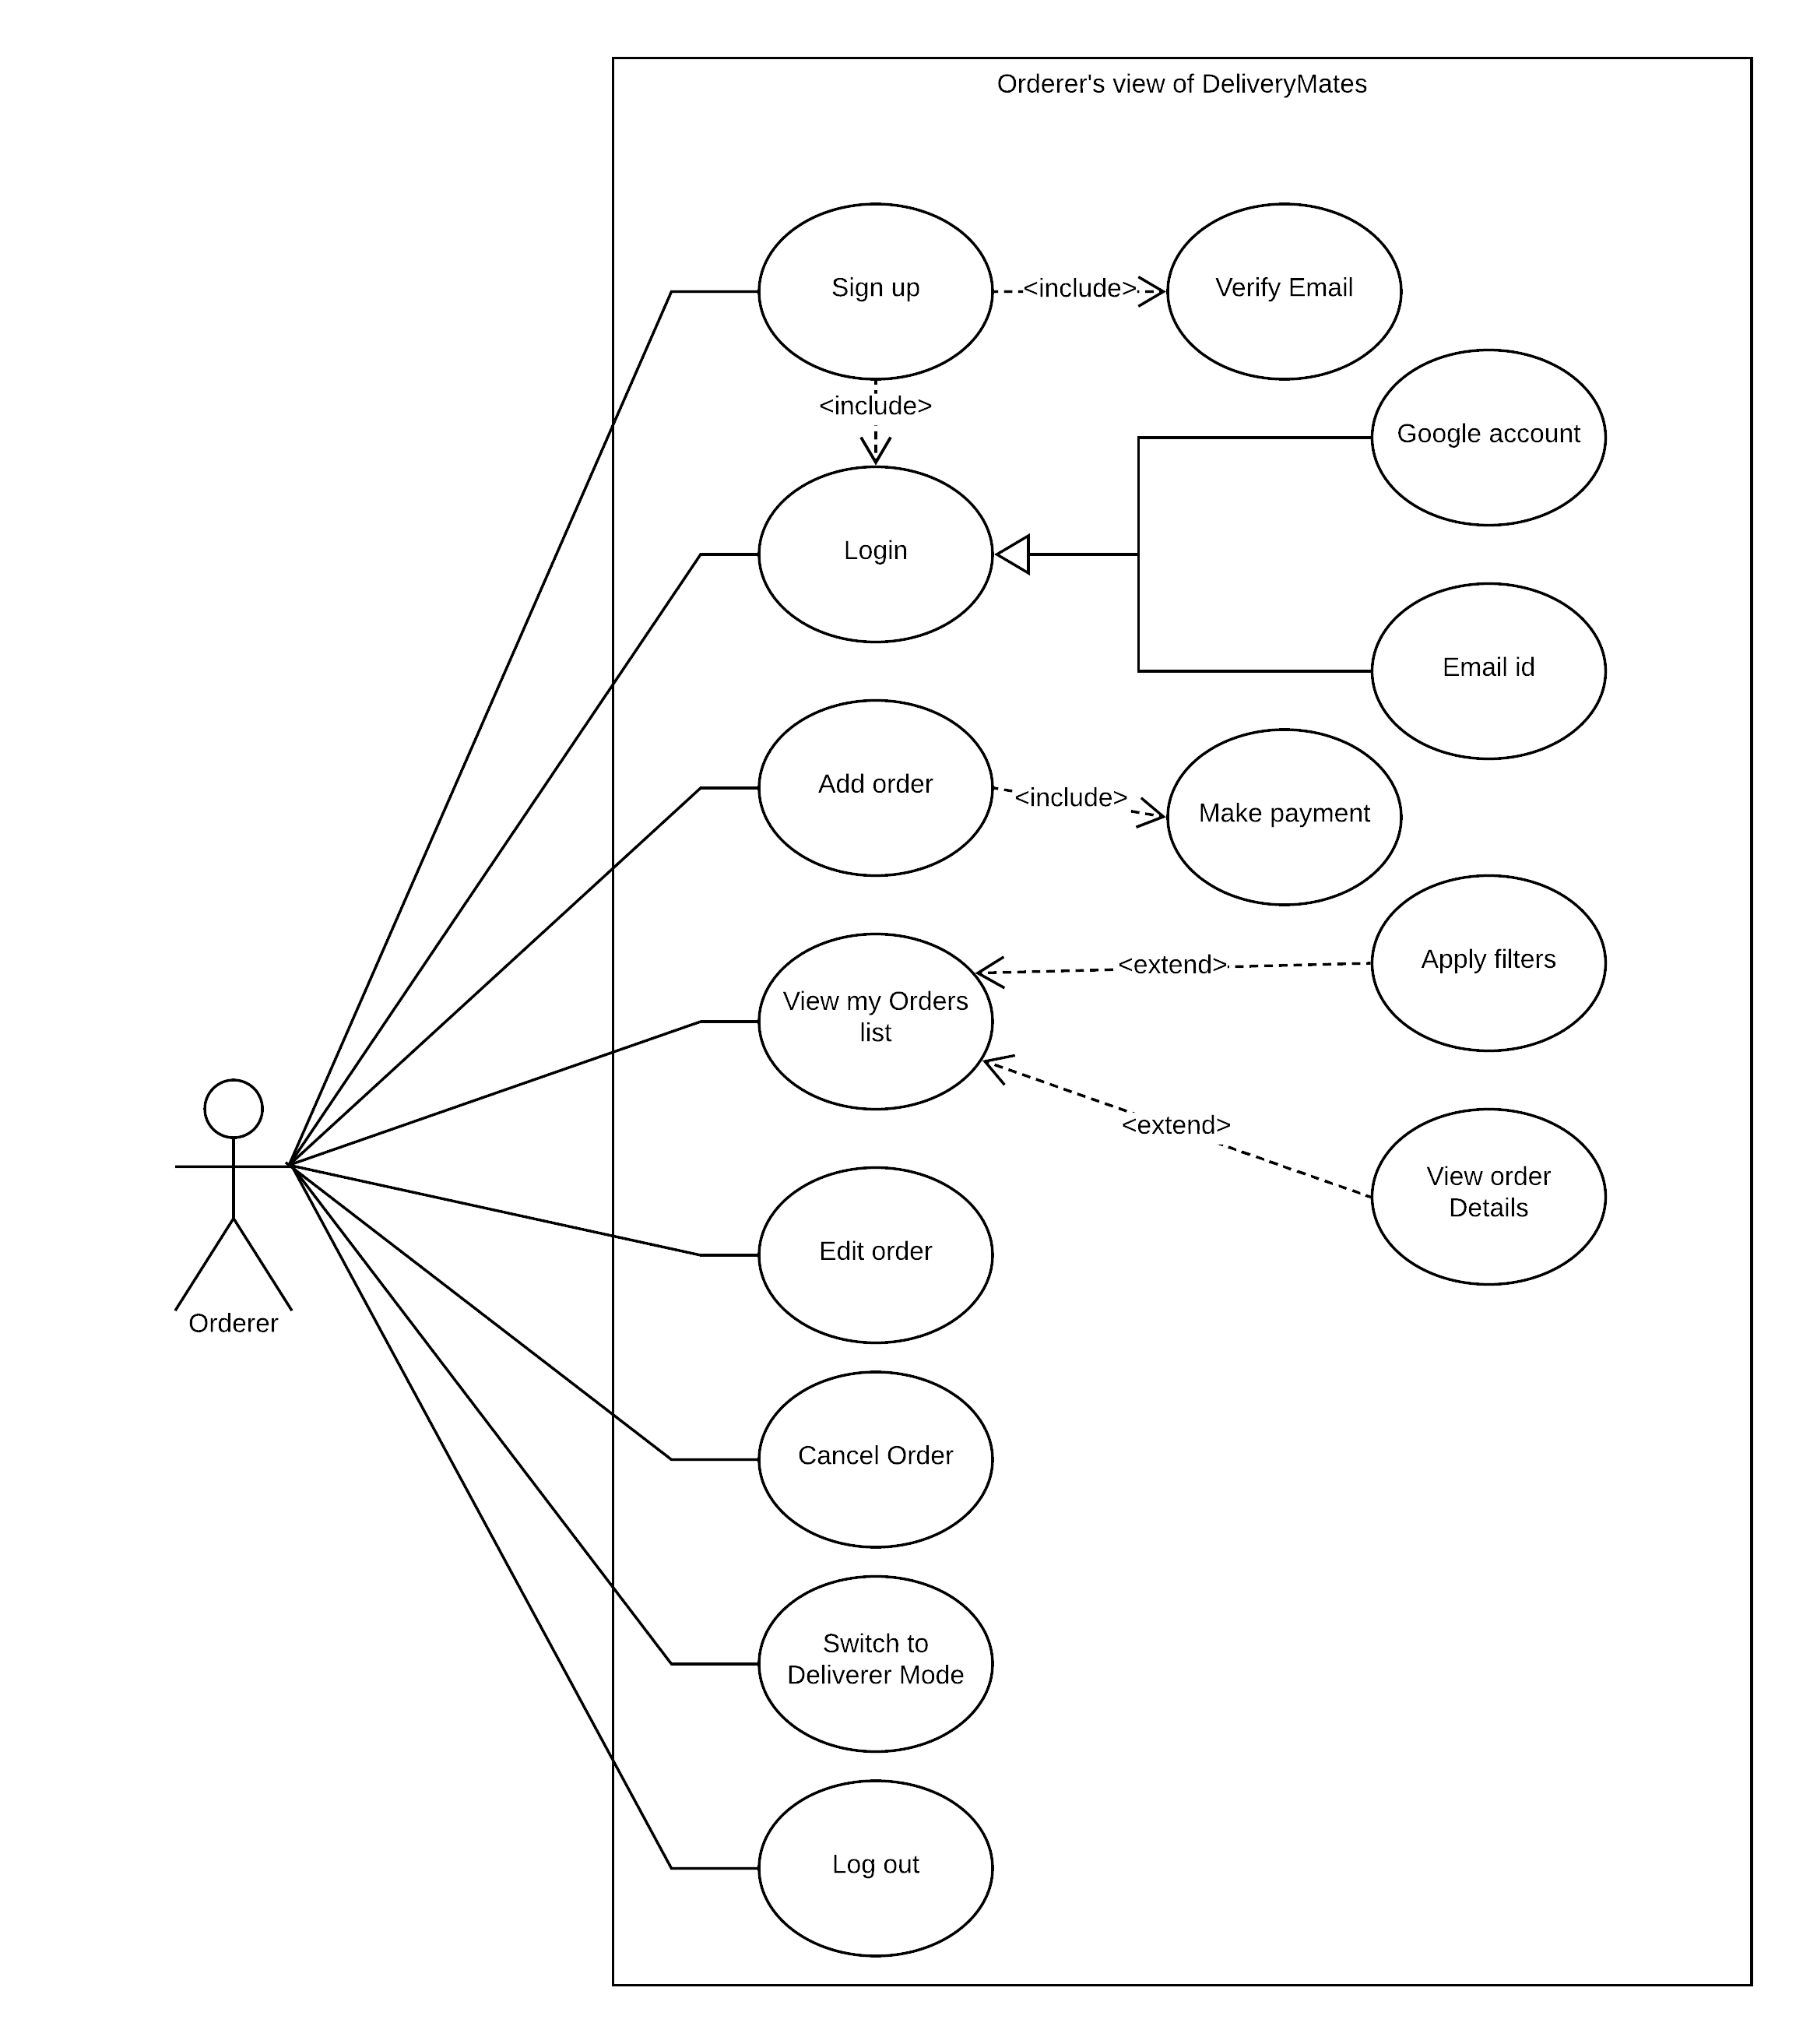
\includegraphics[width=16cm]{OrdererUseCase.png}
\caption{Use case diagram with shopper as an actor in our app}
\label{fig:NASA_Logo}
\end{figure}

\begin{figure}[h!]
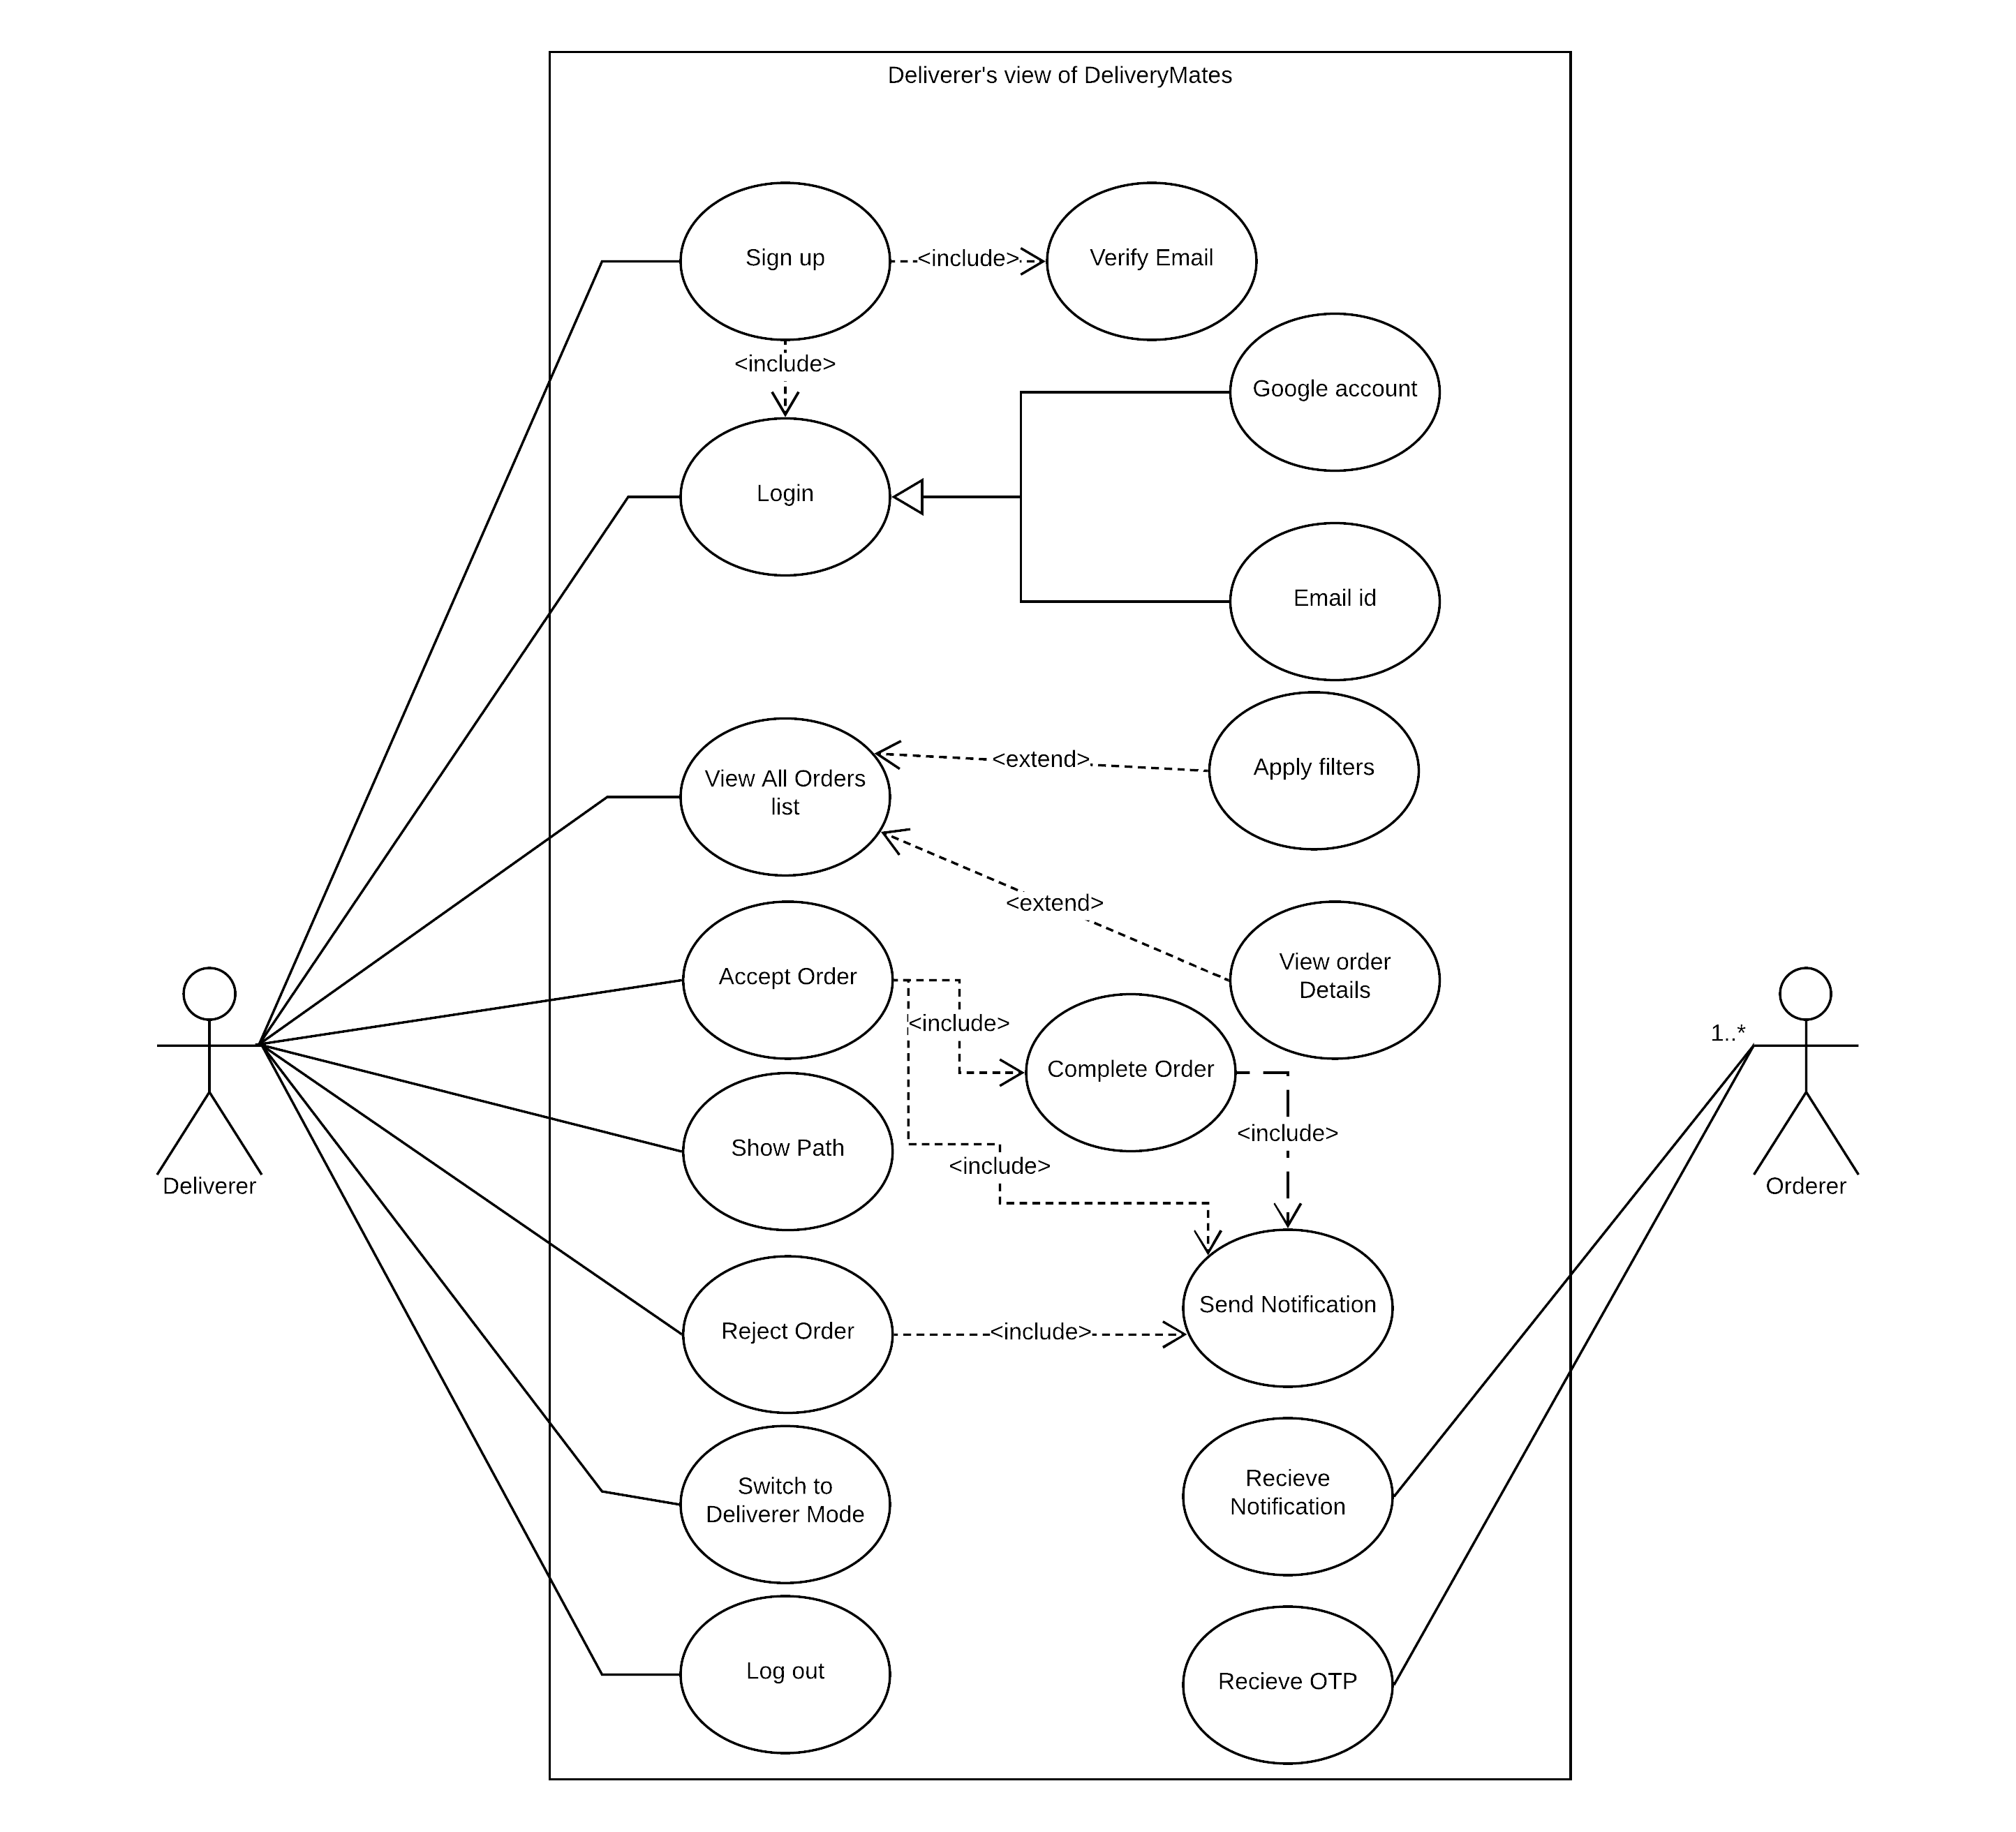
\includegraphics[width=16cm]{DelivererUseCase.png}
\caption{Use case diagram with deliverer as primary actor in our app}
\label{fig:NASA_Logo}
\end{figure}

%--------------------------------------------------------------------------

\chapter{Application Design}

\section{UI Design}
We have made an android application which helps people shop from local stores. Using our application you can order any goods or food items and it will be delivered to you by one of our deliverer.\\

As our app is a kind of a transportation app, we initially thought of making the user interface similar to that of the \textbf{OLA} app.\\
The operations would have been like follows:\\

For placing a new order:
\begin{itemize}
\item A map would have been there which will show all the deliverers, out of which a deliverer would be alloted to us for our delivery.
\item the selected deliverer would be notified of our order and that deliverer would buy our order and deliver it to us at the location chosen at the time of placing the order.
\end{itemize}

But that would type of interface would have brought a lot of problems like:
\begin{itemize}
\item As the deliverer is selected randomly and not of his free will, there are high chances of order rejection, as that deliverer may not want to go to the place from where the order is to be purchased or does not intend to go to the delivery location.
\item The deliverer may not want to deliver your order because of low delivery charge (delivery incentive).
\item So, we may have to get our order rejected a lot of times before we could actually get a deliverer who is willing to deliver our order to us.
\end{itemize}

So, we needed to ensure that the deliverer \textbf{chooses} to deliverer our order.\\
\newline
We solved these problems by choosing a different User interface:\\
The new operations are like follows:\\
For placing a new order:
\begin{itemize}
\item Instead of using a map and choosing a deliverer at the time of placing the order, we created a list of all pending orders, just like unread mails in \textbf{google mail\cite{c6}}. This method also reduces our dependency on google apis which are costly.
\item We also have filters for pending , active , cancelled , finished and expired orders which can be compared with different kind of mail filters we have in gmail\cite{c6} app like inbox , outbox , drafts , social etc.
\item So now every newly placed order will be placed in the list of pending orders which is a global list visible to all the users using our app as a deliverer.
\item All deliverers can check the details of your order, and the deliverers who are interested in delivering your order will \textbf{Accept} your order and will deliver it to you.
\item You will be notified of  as soon as someone \textbf{Accepts} your order.
\end{itemize}
This list of pending orders is implemented using \textbf{Recycler View of cards} which is a very efficient method for displaying a big list of objects in any android application.

\subsection{Login Screen}
\begin{itemize}
\item This is the first screen which is displayed when the app is opened.
\item There are two methods for login:
\begin{itemize}[label=$\rightarrow$]
\item E-mail \& Password
\item Google Sign-in
\end{itemize}
\end{itemize}

\begin{figure}[h!]
\begin{subfigure}[b]{.26\textwidth}
\centering
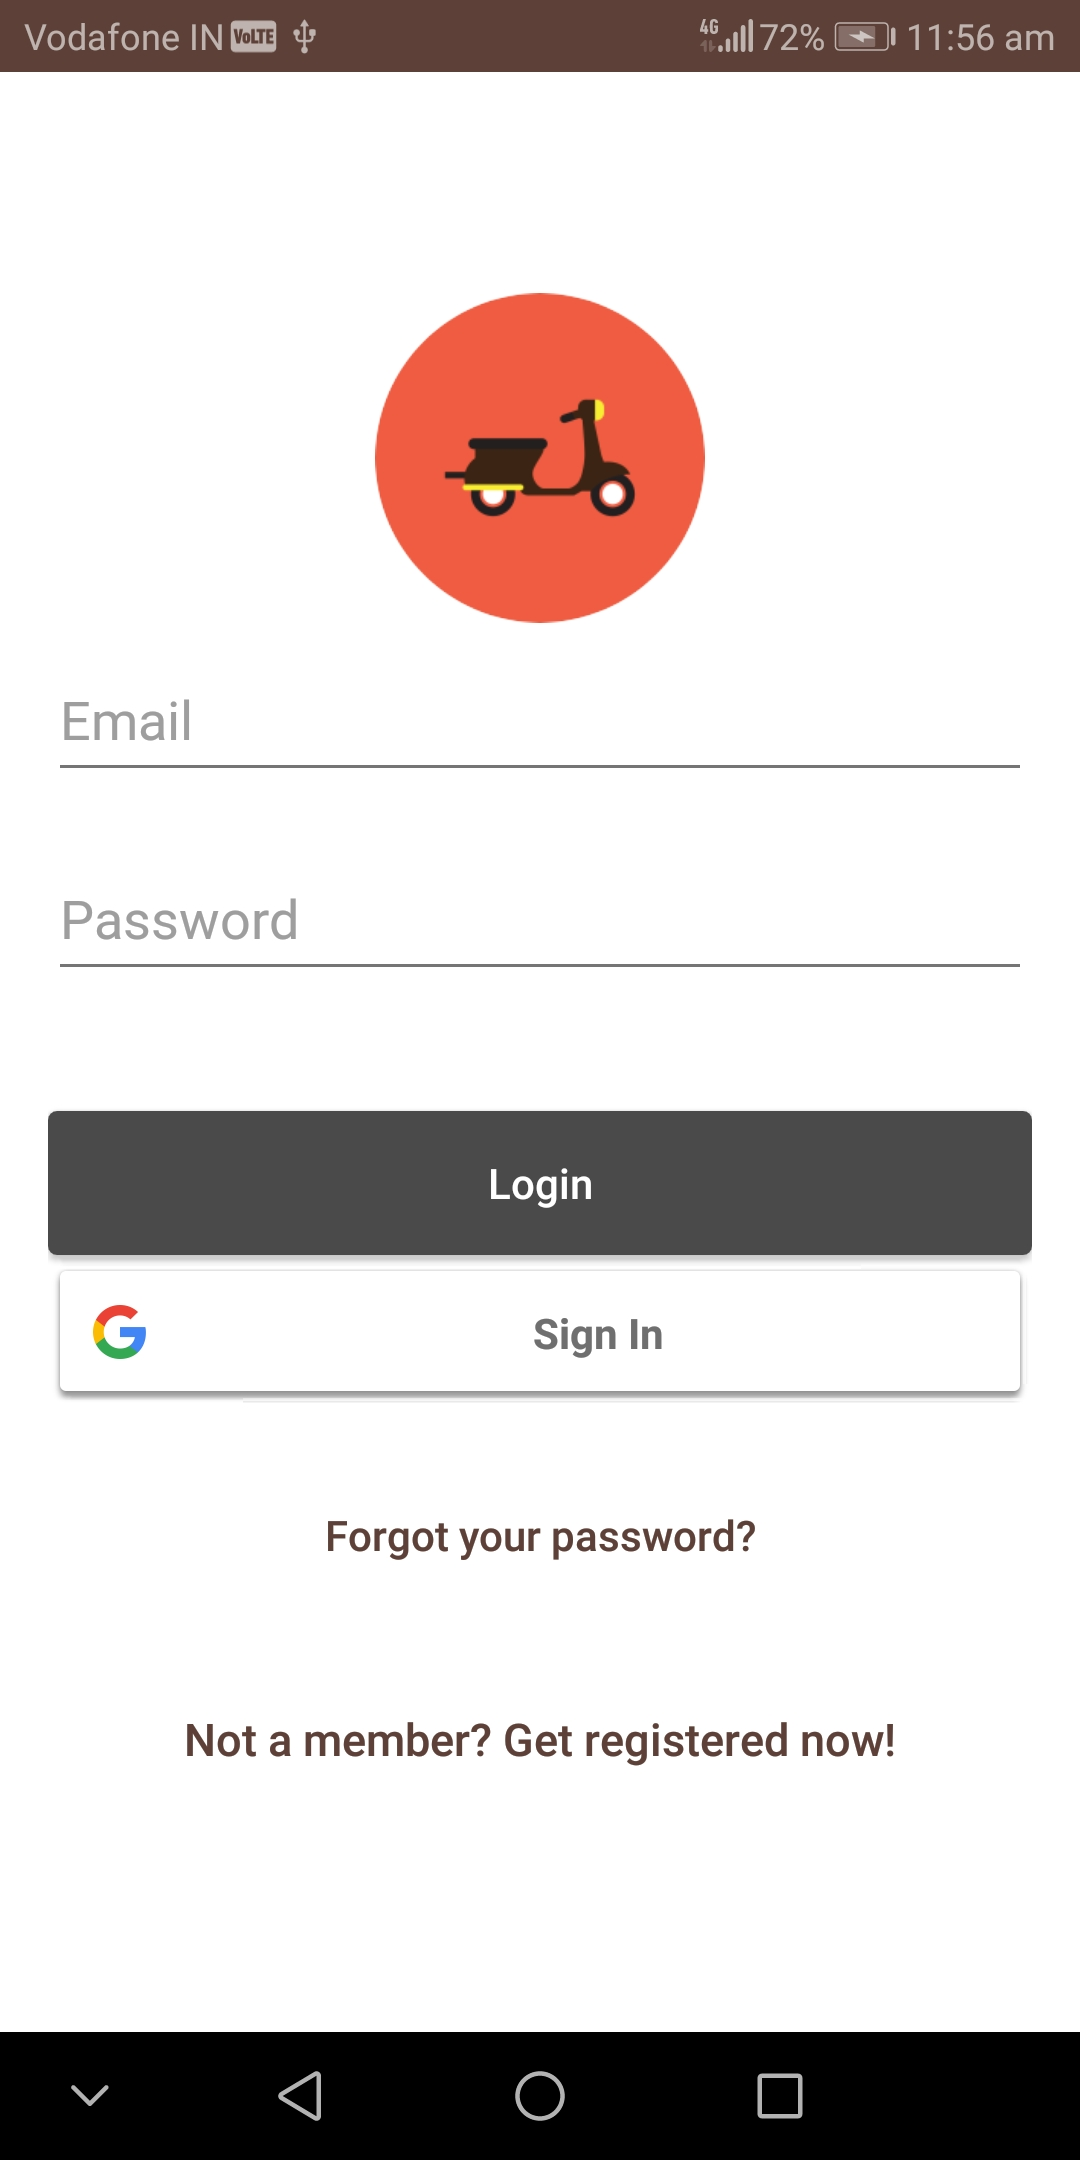
\includegraphics[width=4.2cm]{login.jpg}
\caption{\centering Login screen using E-Mail \& Password}
\end{subfigure}
\begin{subfigure}[b]{.26\textwidth}
\centering
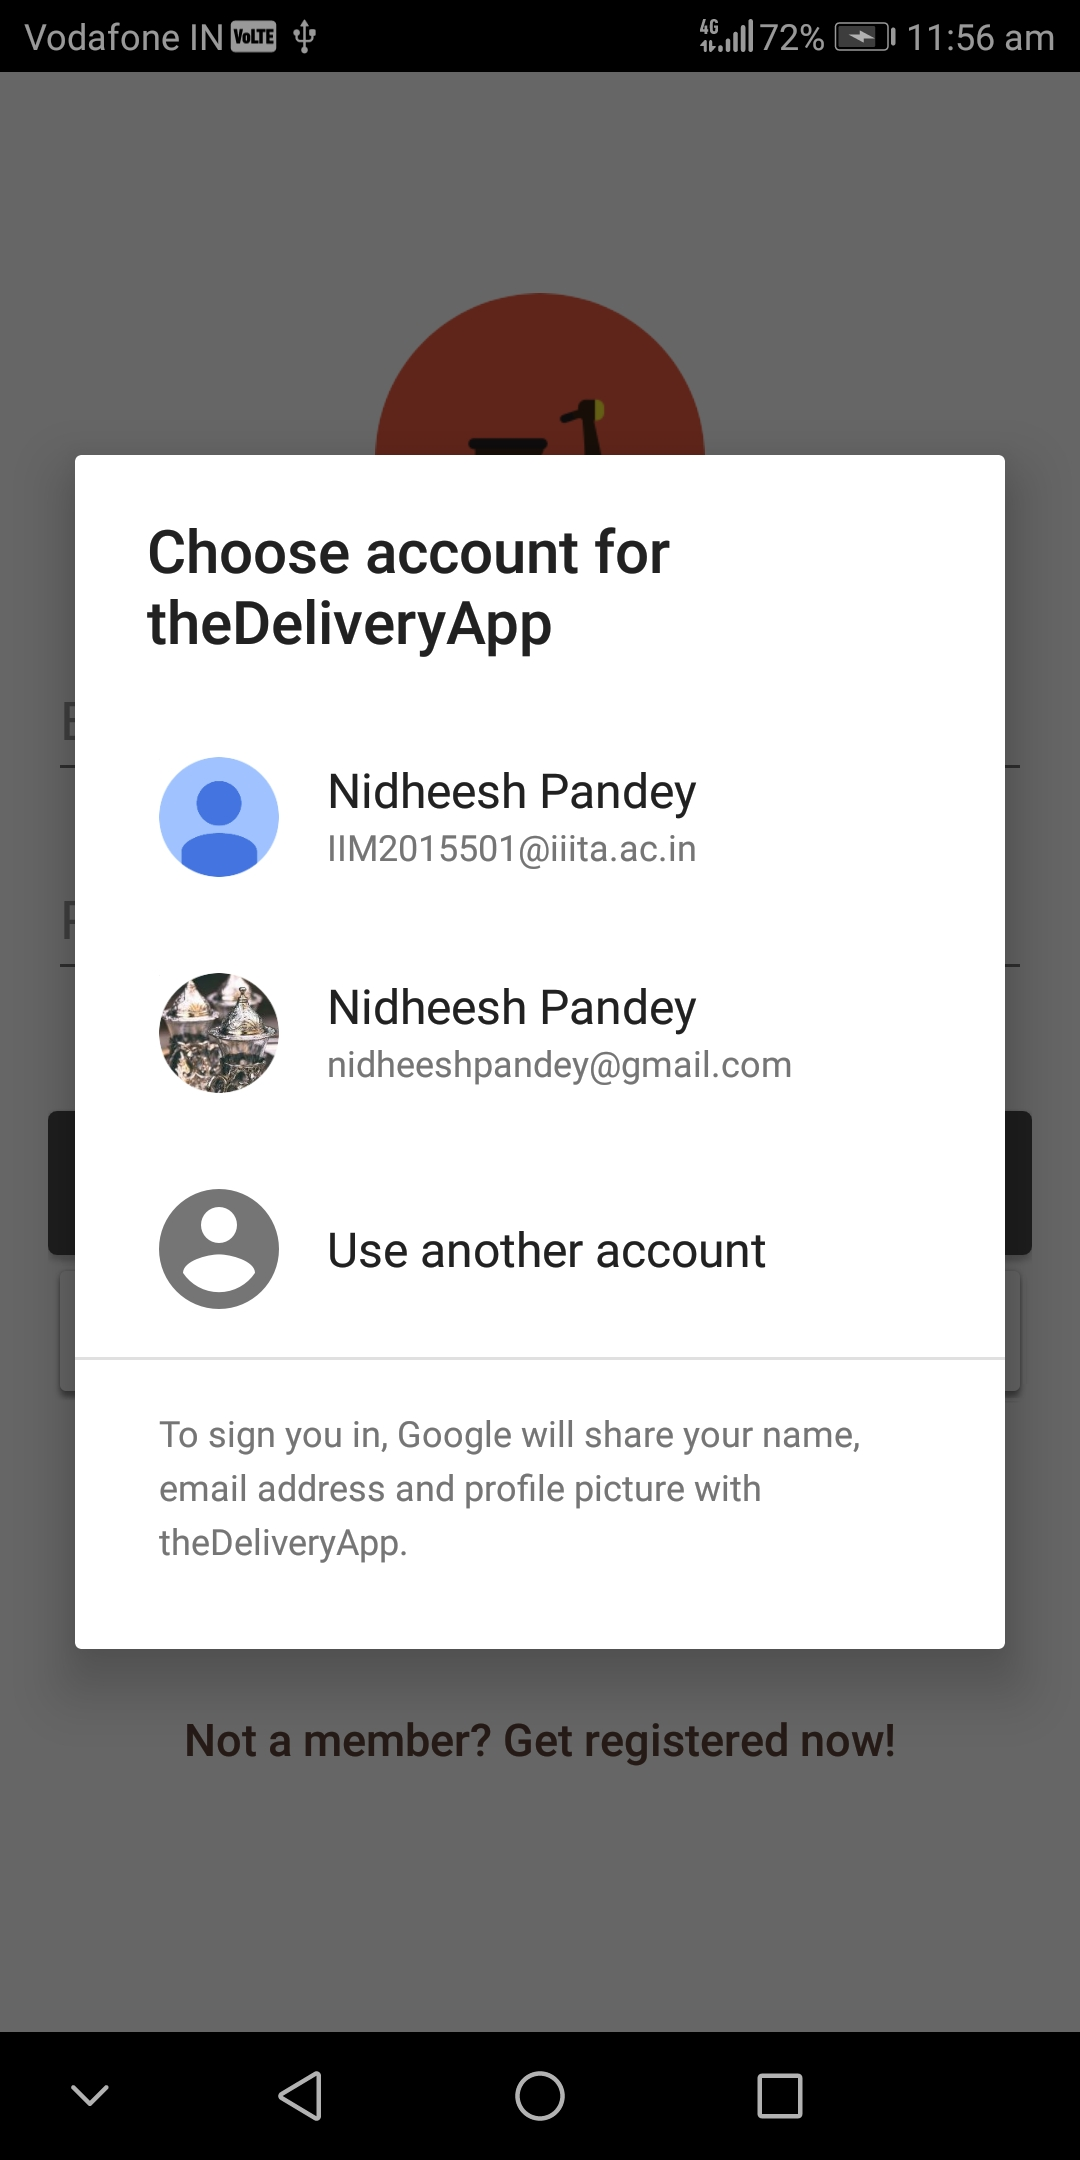
\includegraphics[width=4.2cm]{google_signin.jpg}
\caption{\centering Reset Password screen}
\end{subfigure}
\begin{subfigure}[b]{.26\textwidth}
\centering
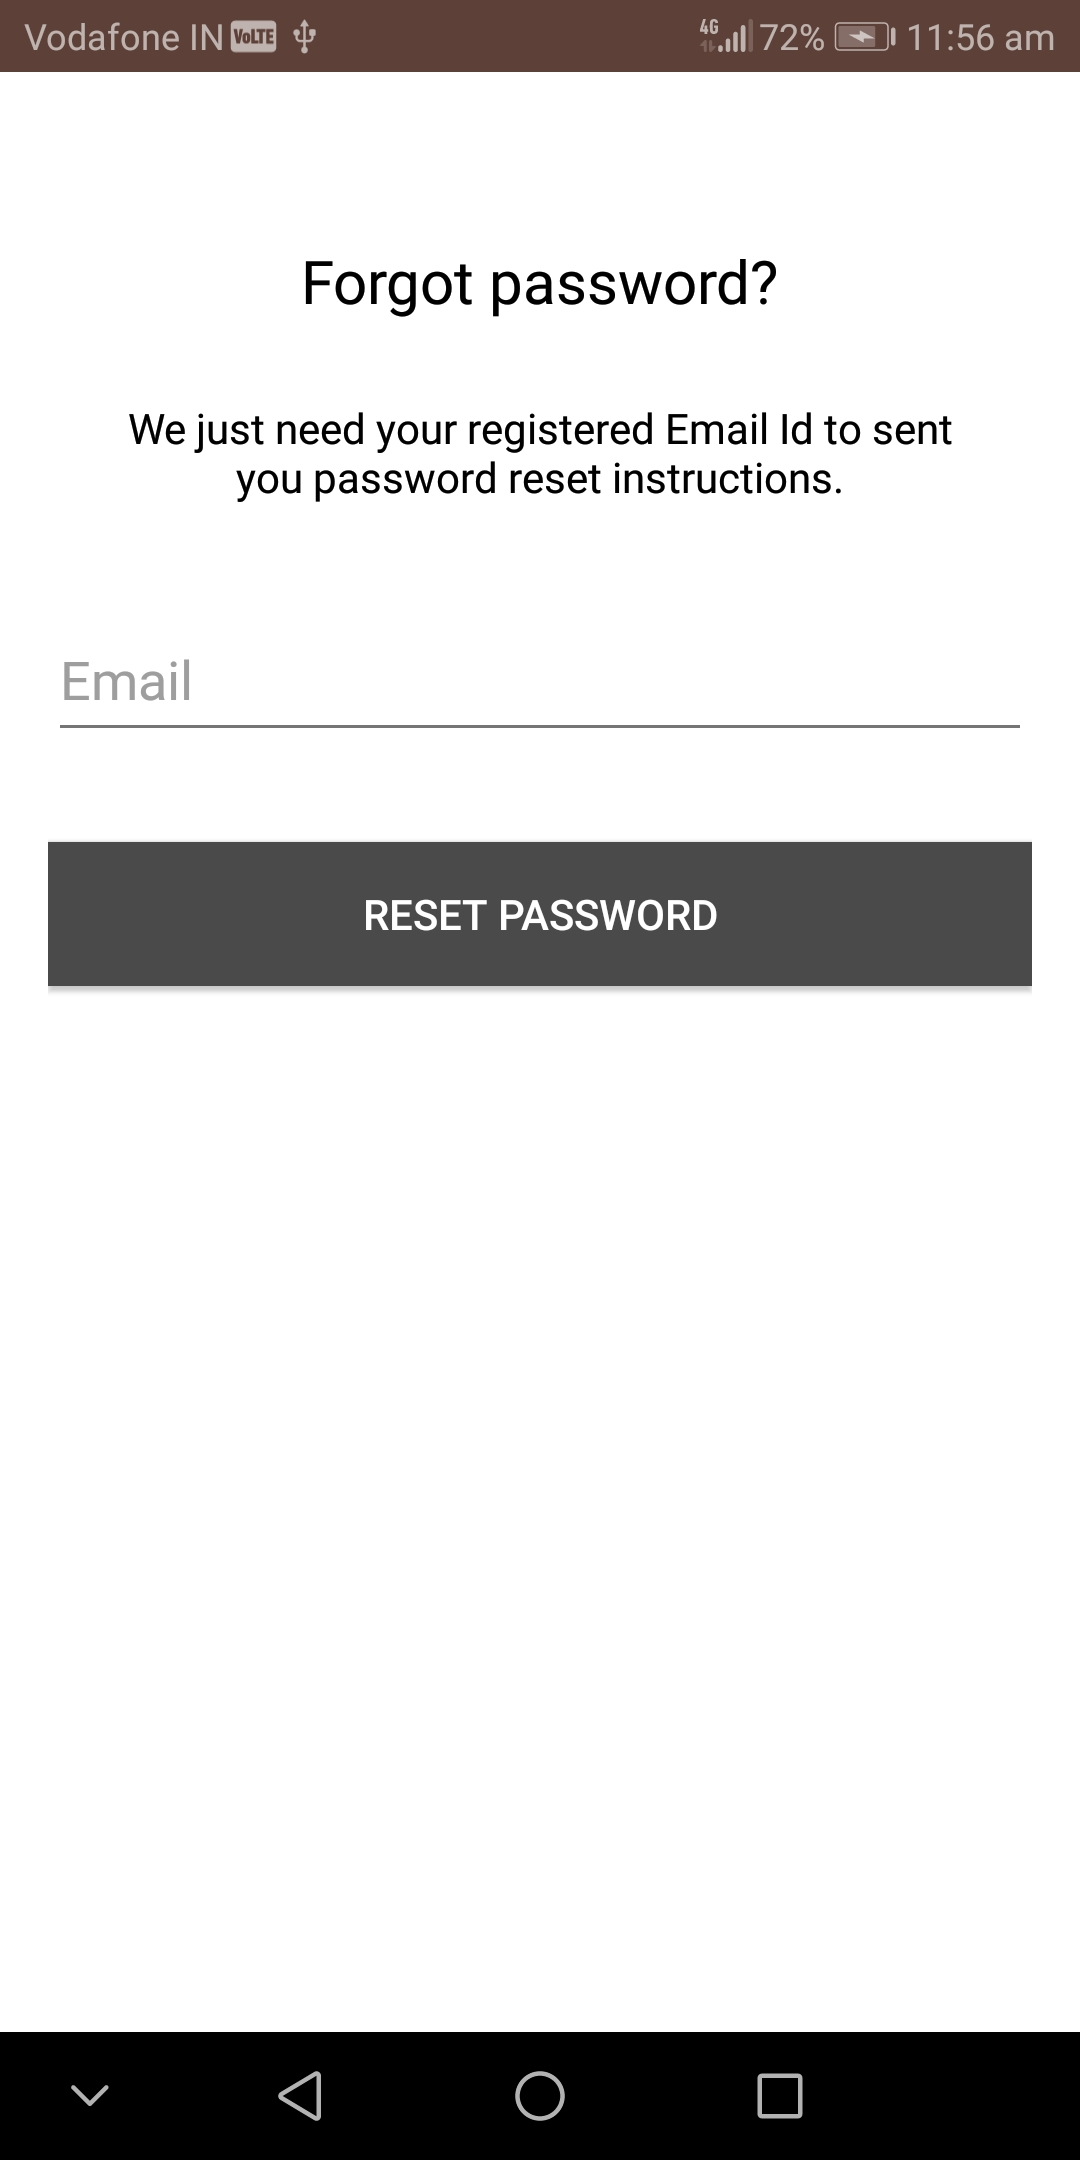
\includegraphics[width=4.2cm]{forgot_password.jpg}
\caption{\centering Forgot password screen}
\end{subfigure}
\caption{Login Screen and Password Reset} 
\label{fig:NASA_Logo}
\end{figure}

\pagebreak

\subsection{Forgot Password Screen}
\begin{itemize}
\item If you ever forget your password, just enter your registered E-mail and the password reset instructions will be sent to that E-mail.
\end{itemize}


\subsection{New Registration Screen}
\begin{itemize}
\item This is the screen for registration for the E-mail \& Password method in our database.
\end{itemize}


\begin{figure}[h!]
\begin{subfigure}[b]{.3\textwidth}
\centering
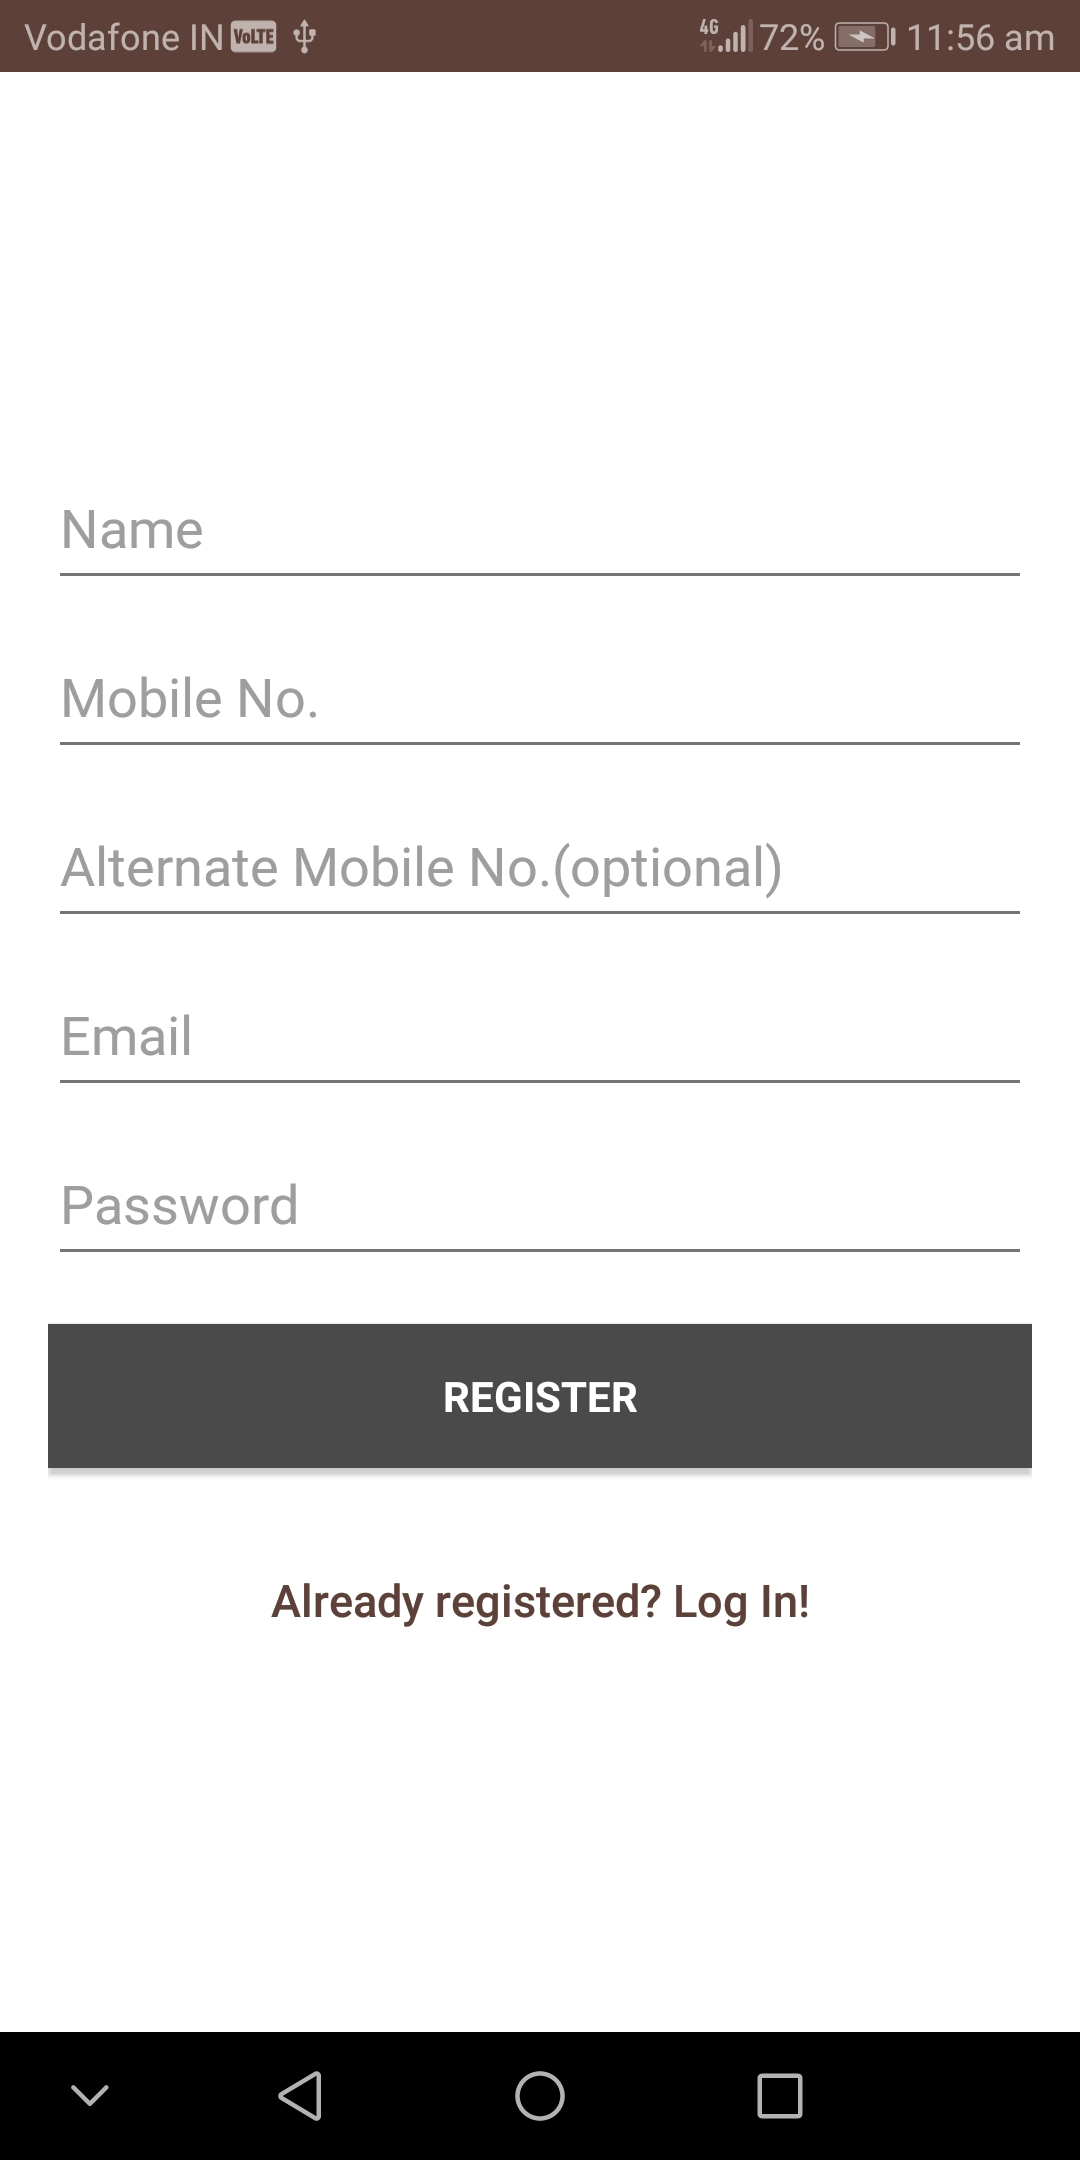
\includegraphics[width=5cm]{signup.jpg}
\caption{\centering User Registration form}
\end{subfigure}
\begin{subfigure}[b]{.3\textwidth}
\centering
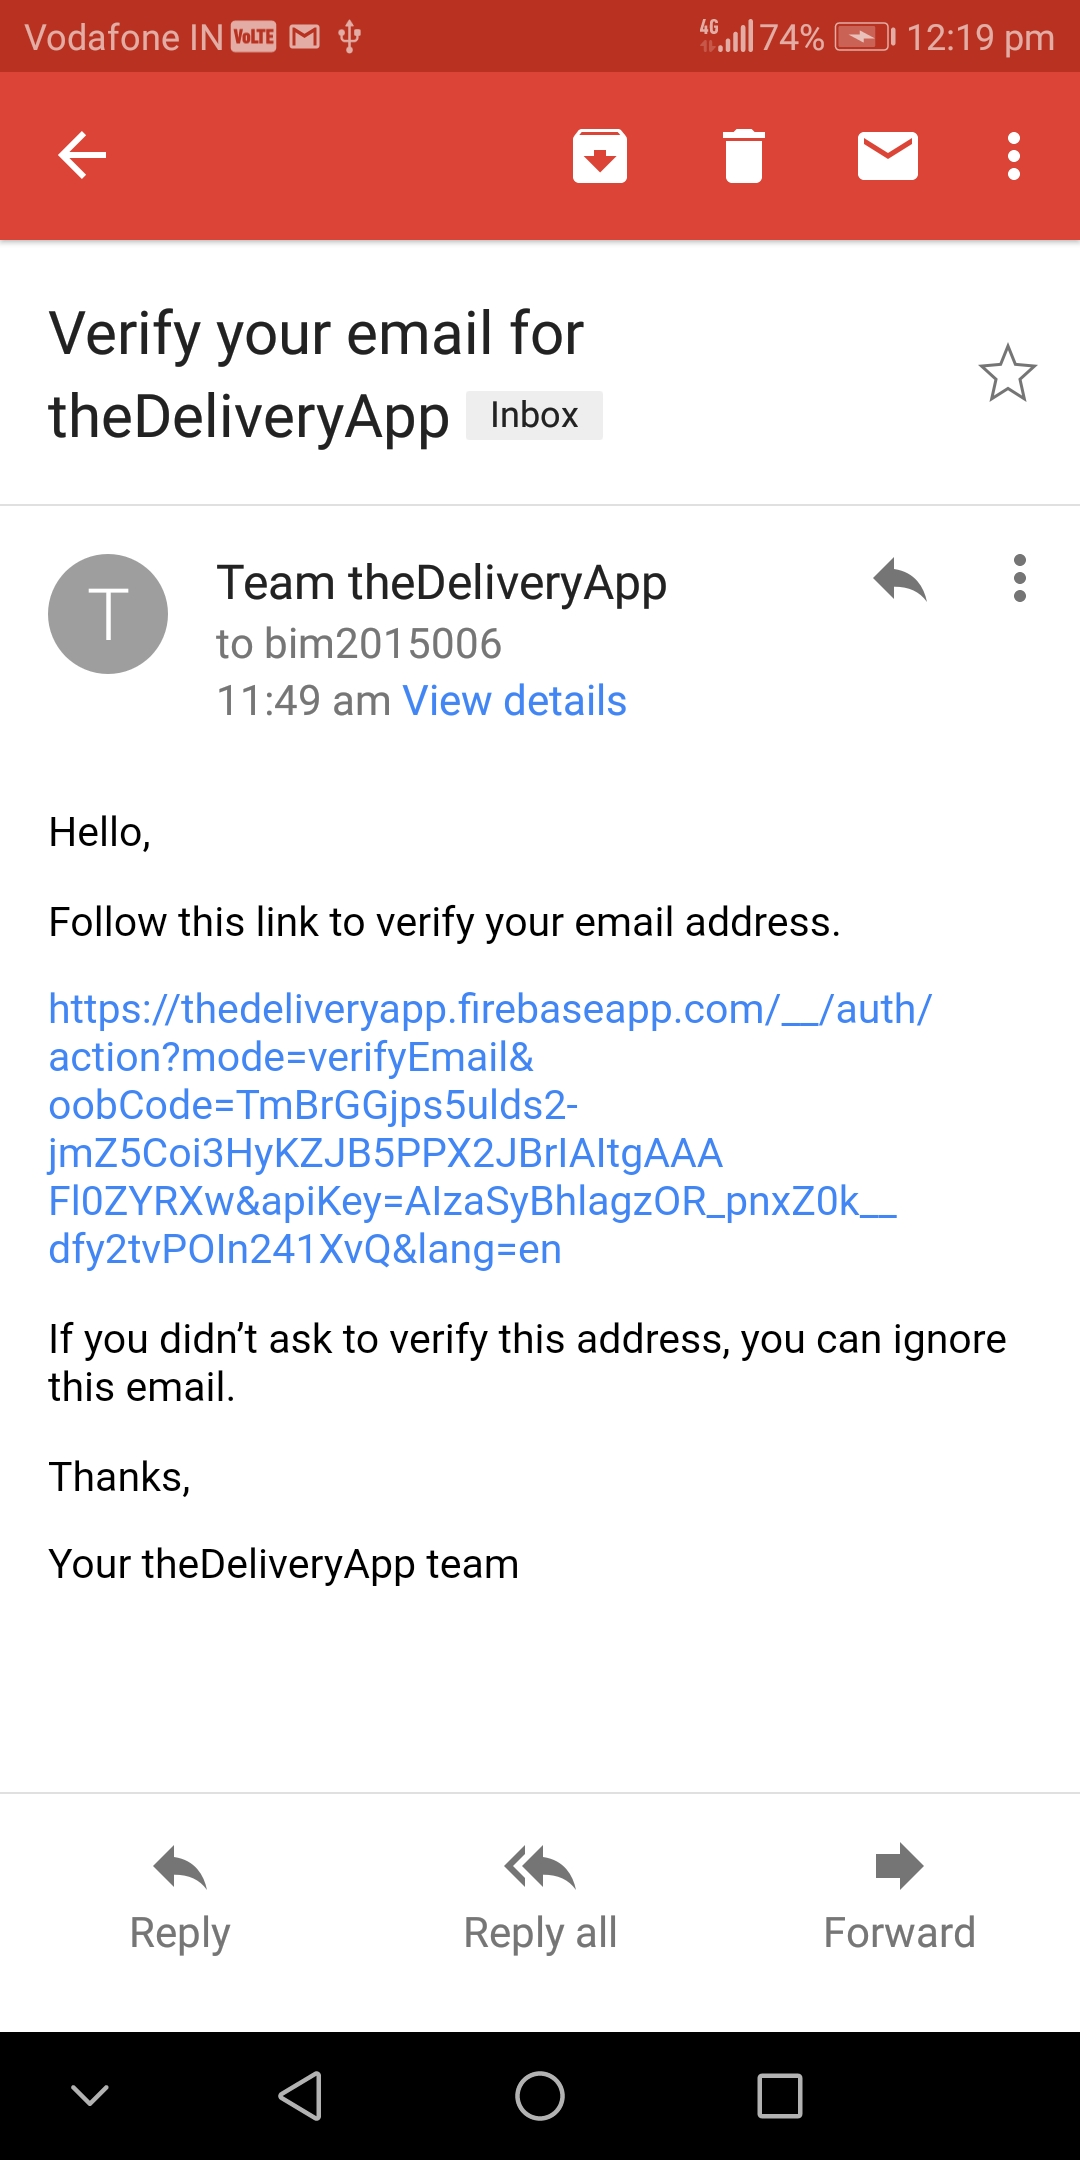
\includegraphics[width=5cm]{verify_email.jpg}
\caption{\centering E-Mail verification Mail}
\end{subfigure}
\caption{Registration screen and E-Mail verification mail} 
\label{fig:NASA_Logo}
\end{figure}


\subsection{Choose Mode of Usage}
\begin{itemize}
\item This is the screen where you choose whether you want to act as a Shopper or as a Deliverer.
\item The interface of both the modes is very similar.
\end{itemize}



\subsection{Shopper View}
\begin{itemize}
\item All of your orders will be displayed in this screen in the form of a Recycler View of cards where each card is used to show an order.
\item The default filter shows all your Pending and Active orders on this screen.
\item Each order is summarised in the form of a card in the Recycler view showing its Status, Category, Description, Maximum range price, Delivery Charge and the Expiry Date \& time.
\item On the top left there is the toolbar menu button for displaying the Navigation Drawer.
\item On the bottom right there is a PLUS Floating Action Button which is used for placing a new order.
\end{itemize}

\begin{figure}[h!]
\begin{subfigure}[b]{.3\textwidth}
\centering
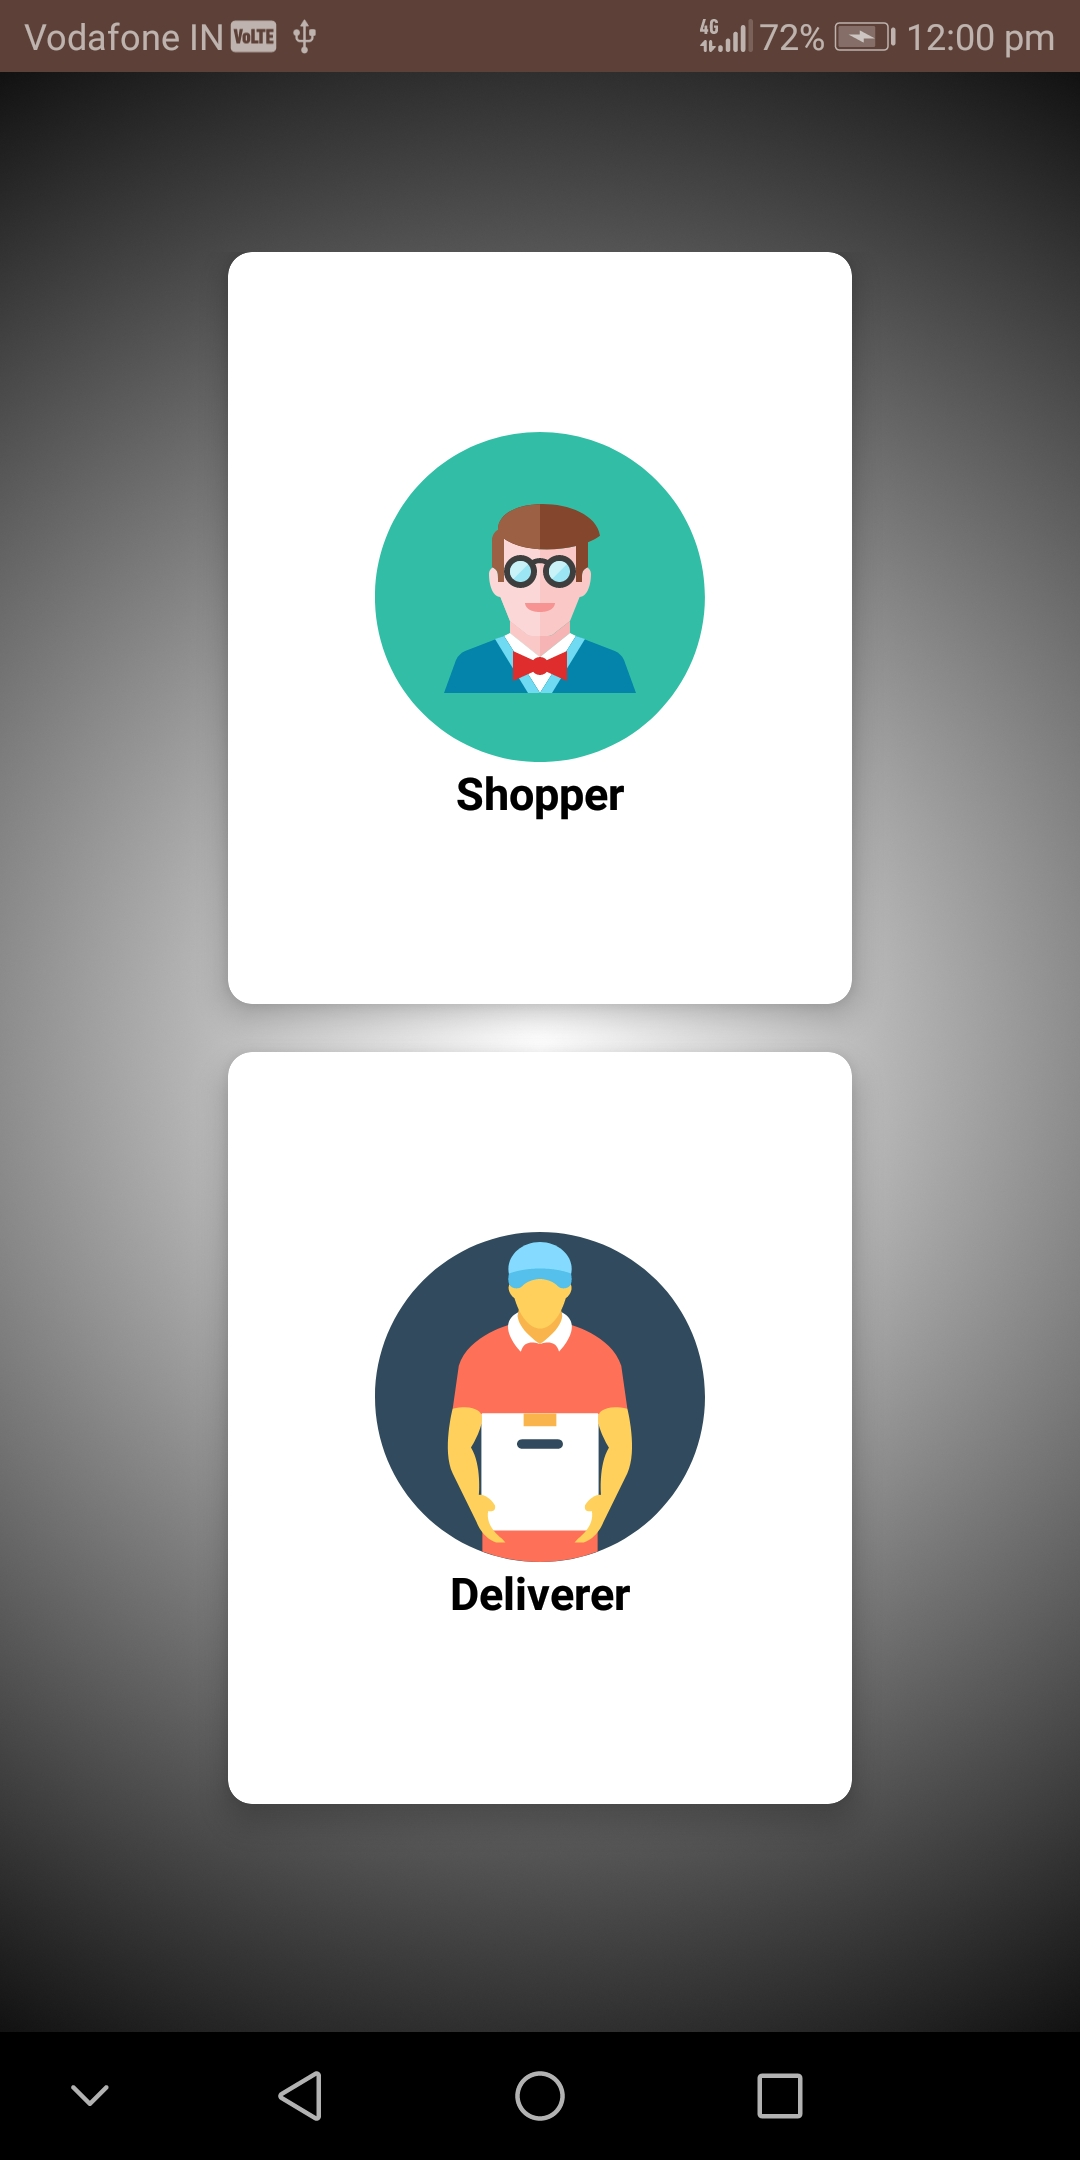
\includegraphics[width=5cm]{main_screen.jpg}
\caption{\centering Usage mode screen}
\end{subfigure}
\begin{subfigure}[b]{.3\textwidth}
\centering
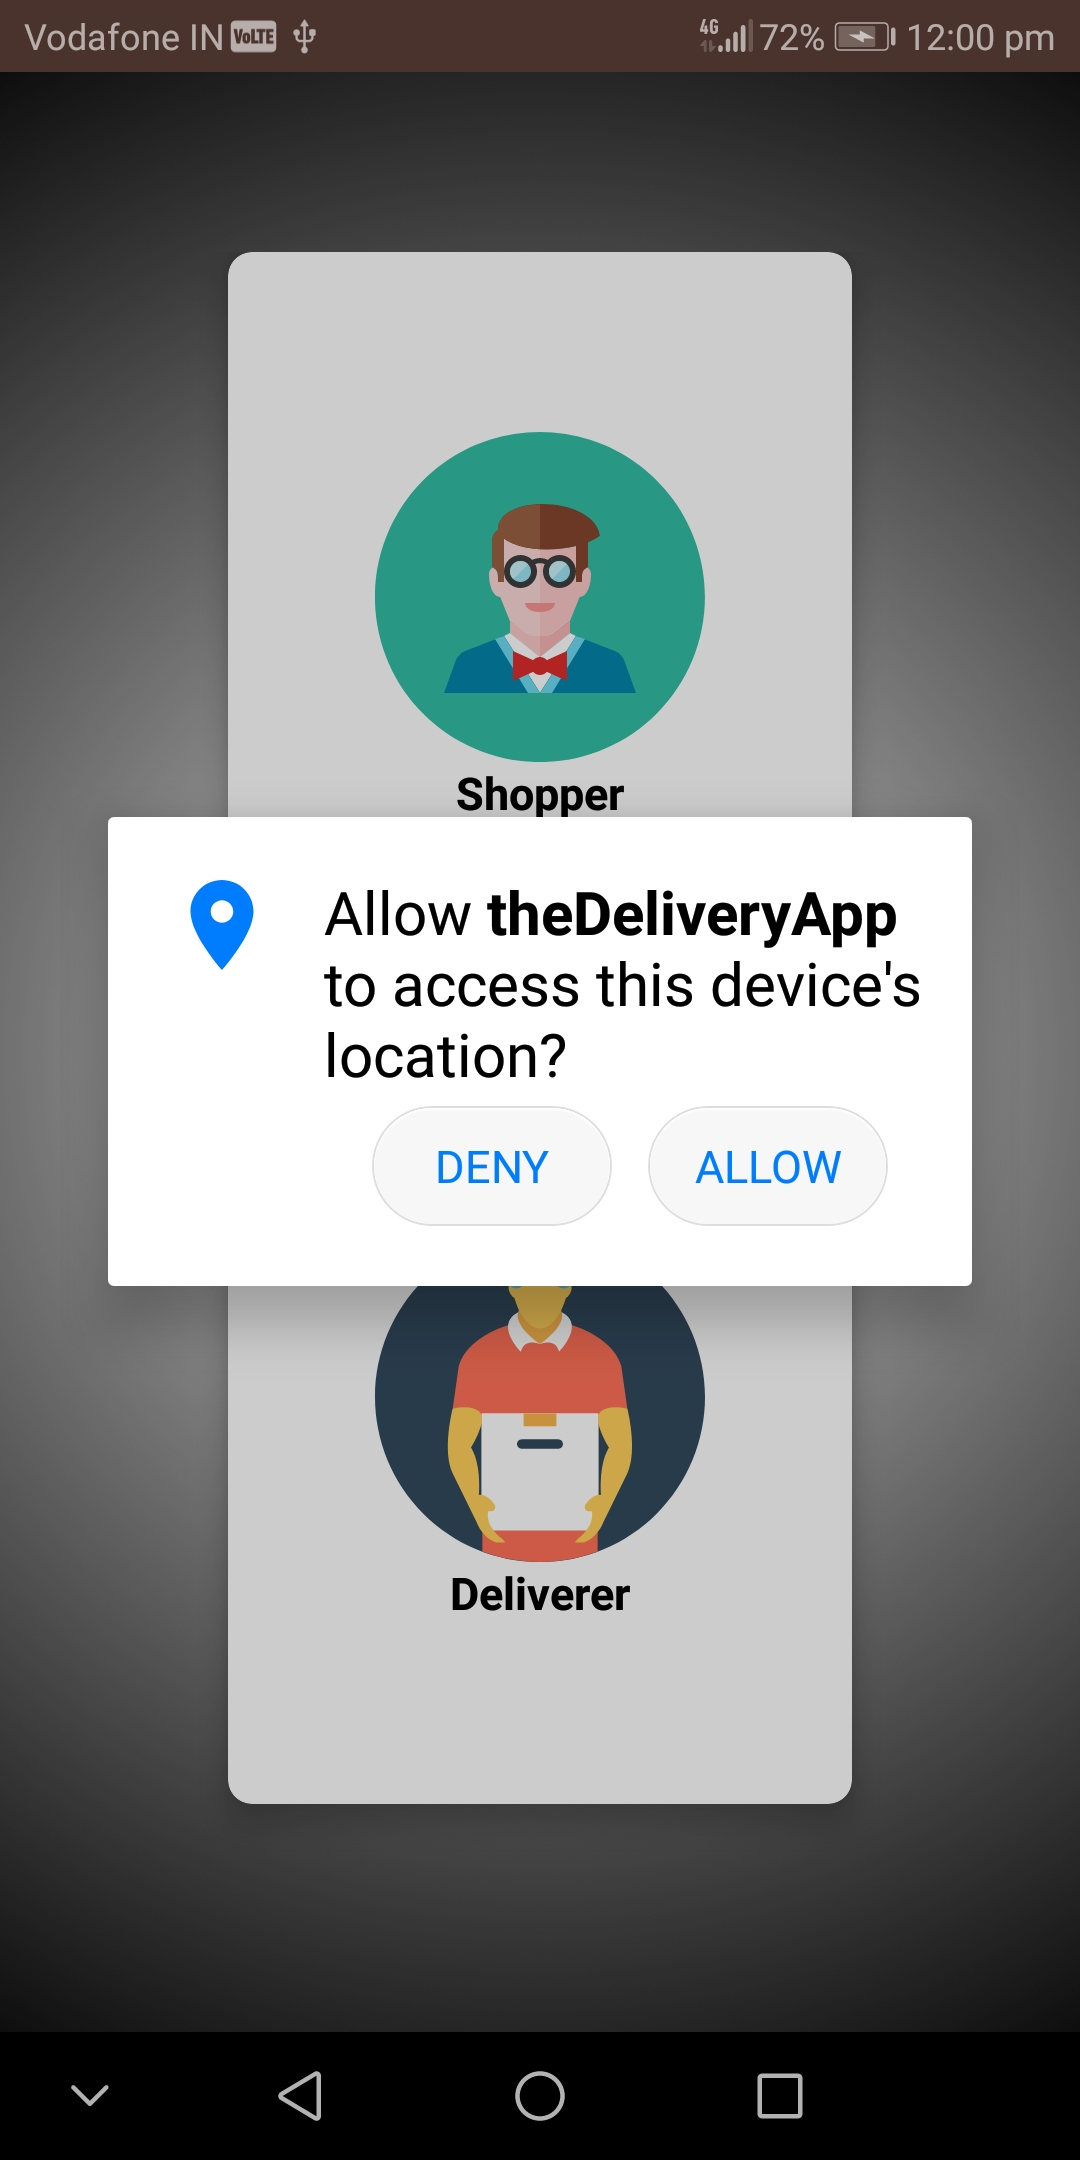
\includegraphics[width=5cm]{location_permission.jpg}
\caption{\centering GPS Location permission}
\end{subfigure}
\begin{subfigure}[b]{.3\textwidth}
\centering
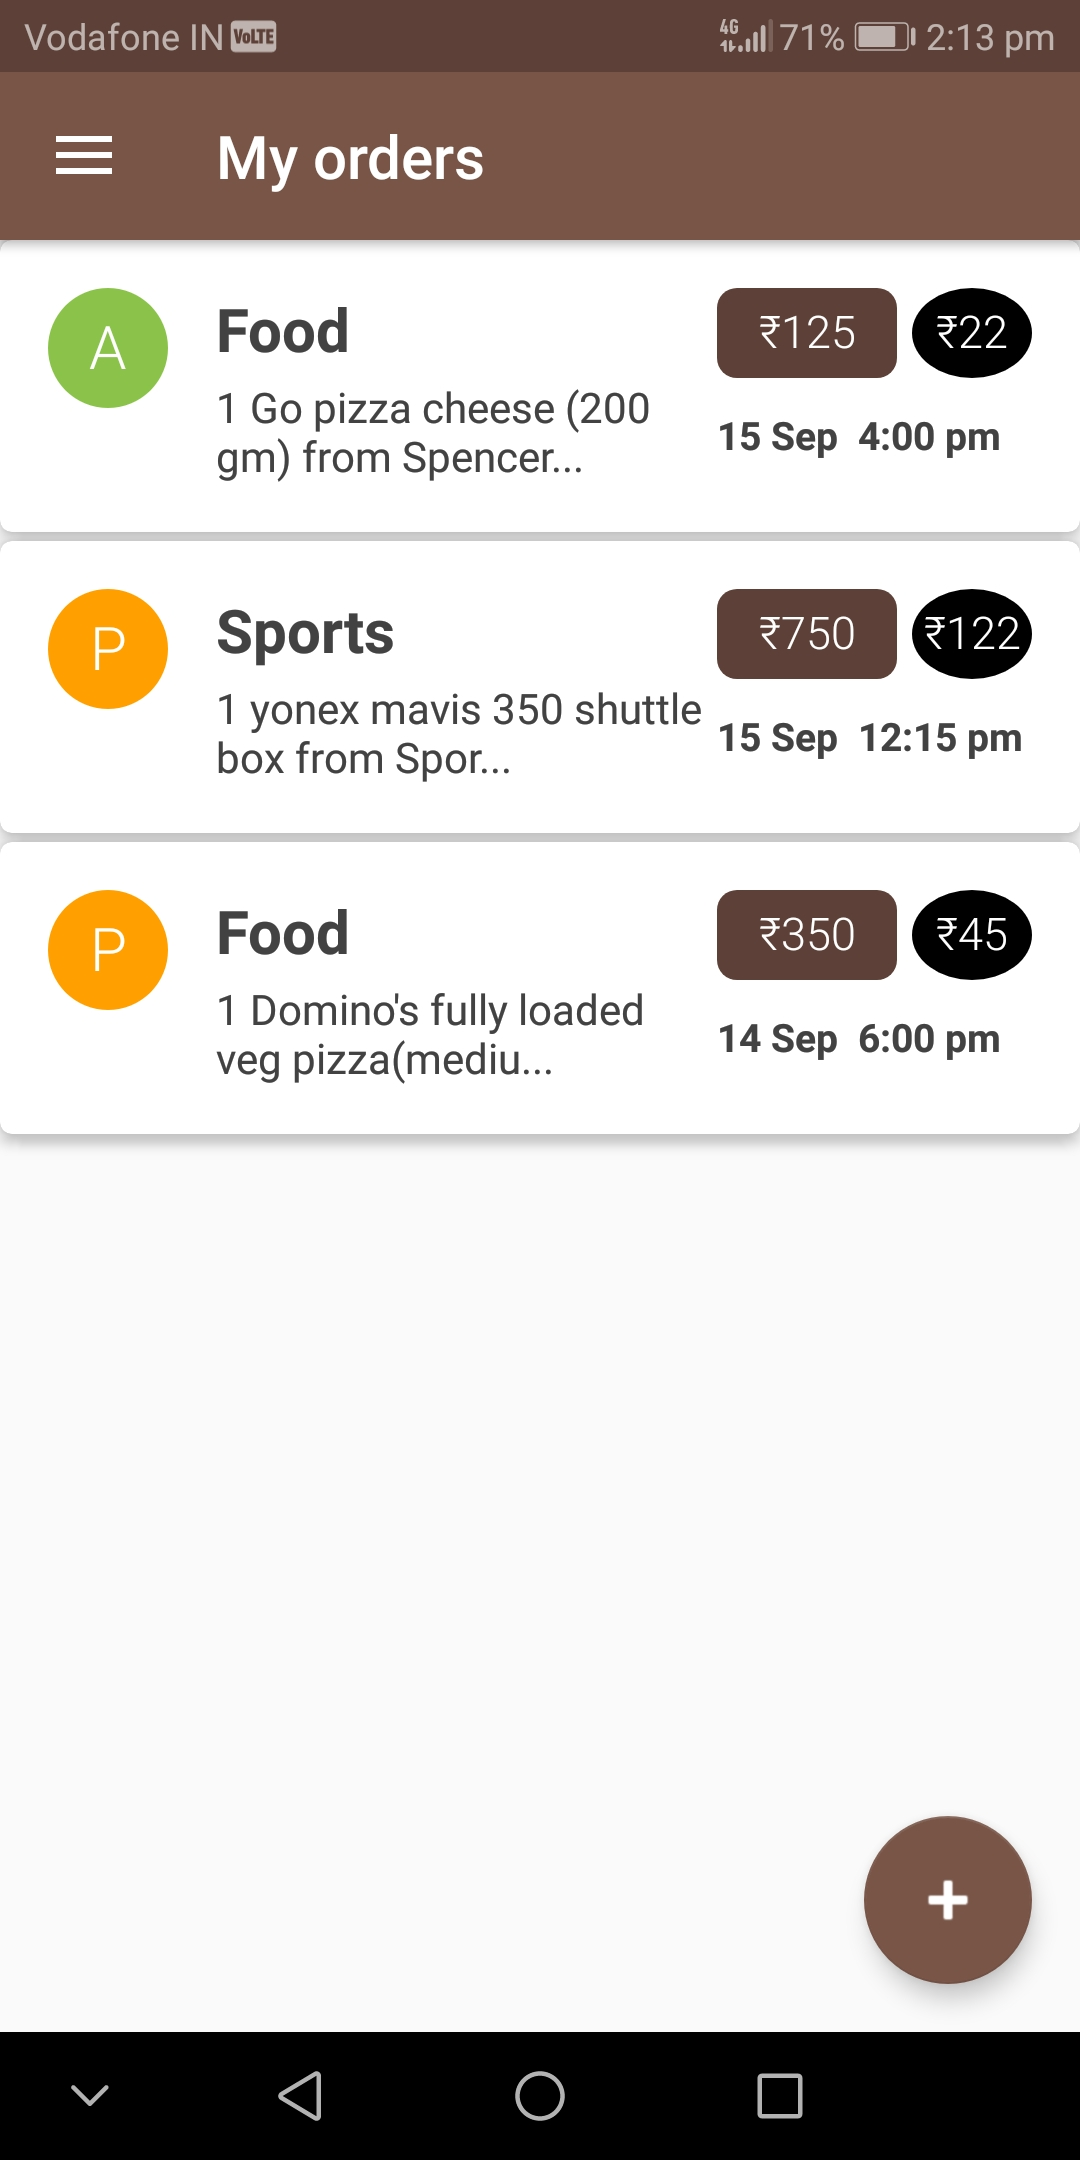
\includegraphics[width=5cm]{shopper_view.jpg}
\caption{\centering Shopper view showing Active \& Pending orders}
\end{subfigure}
\caption{Usage mode screen and Shopper view screen} 
\label{fig:NASA_Logo}
\end{figure}



\subsection{Shopper Order Detail View}
\begin{itemize}
\item Clicking an order in the Shopper View will open the detailed view of that order in a new activity.
\item All the details of that order can be found here in this screen which also contains a nice Collapsing Toolbar Layout.
\item There is also an EDIT floating Action Button on the top right of the screen using which we can edit the details of that order.
\item When an order is accepted, the OTP will also be displayed in this screen and the details of the deliverer will also be shown.
\end{itemize}

\subsection{Shopper Navigation Drawer}
\begin{itemize}
\item Touching the top left toolbar Menu button opens the Navigation Drawer for the Shopper which can also be opened by sliding the screen from the left boundary of the mobile to a slight right.
\item This Navigation Drawer shows your basic profile details along with your current PayTM wallet balance.
\item There is the option to switch to the Deliverer View i.e. use the app as a Deliverer to deliver orders.
\item We also have various filters for order display like All orders, Active, Pending, Finished, Cancelled and Expired orders. Touching any one of them results in the display of only those type of orders(if any) in the Recycler view.
\item On the bottom of the Navigation Drawer is the option to Sign-Out of the app.
\end{itemize}

\begin{figure}[h!]
\begin{subfigure}[b]{.3\textwidth}
\centering
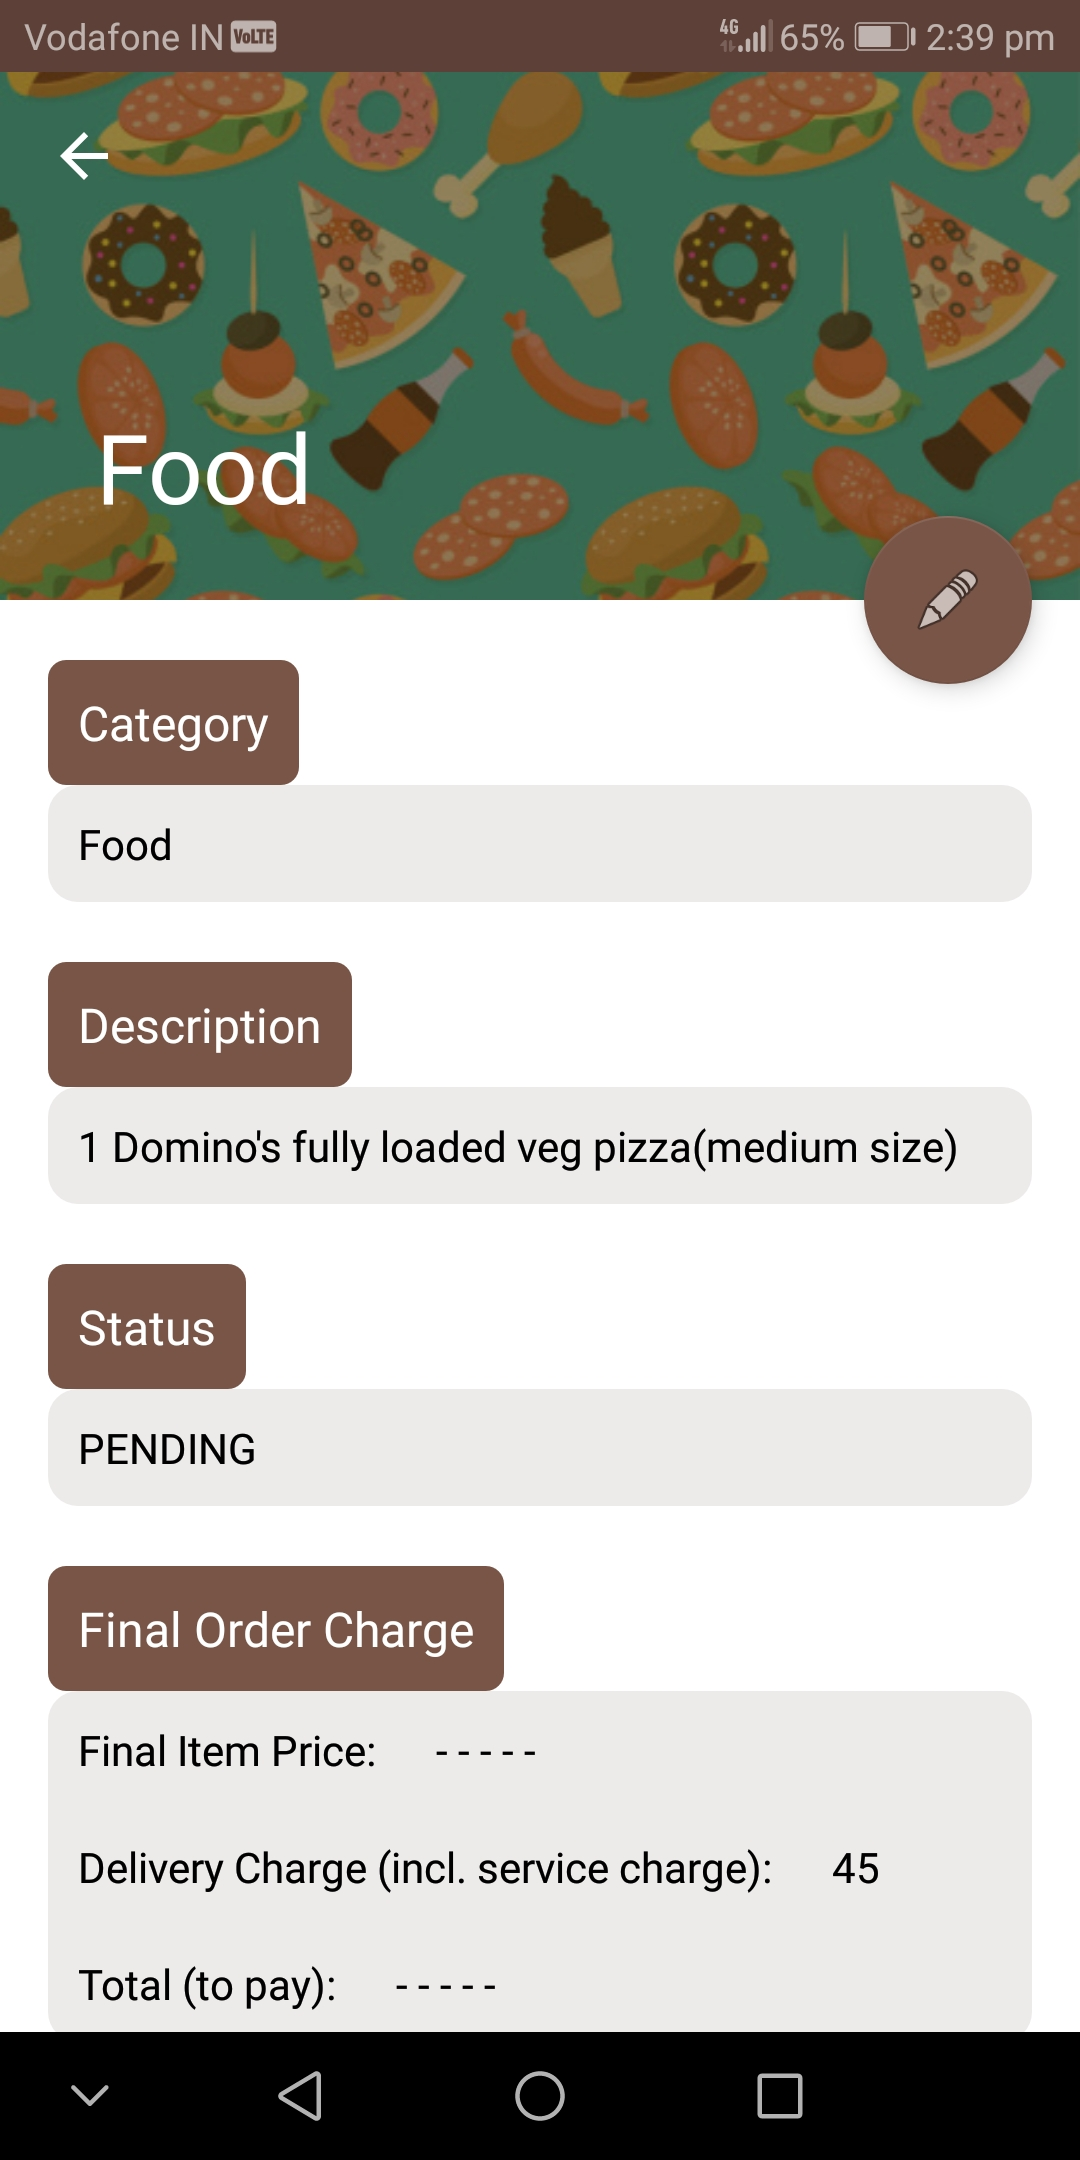
\includegraphics[width=5cm]{order_detail1.jpg}
\caption{\centering Order detail view}
\end{subfigure}
\begin{subfigure}[b]{.3\textwidth}
\centering
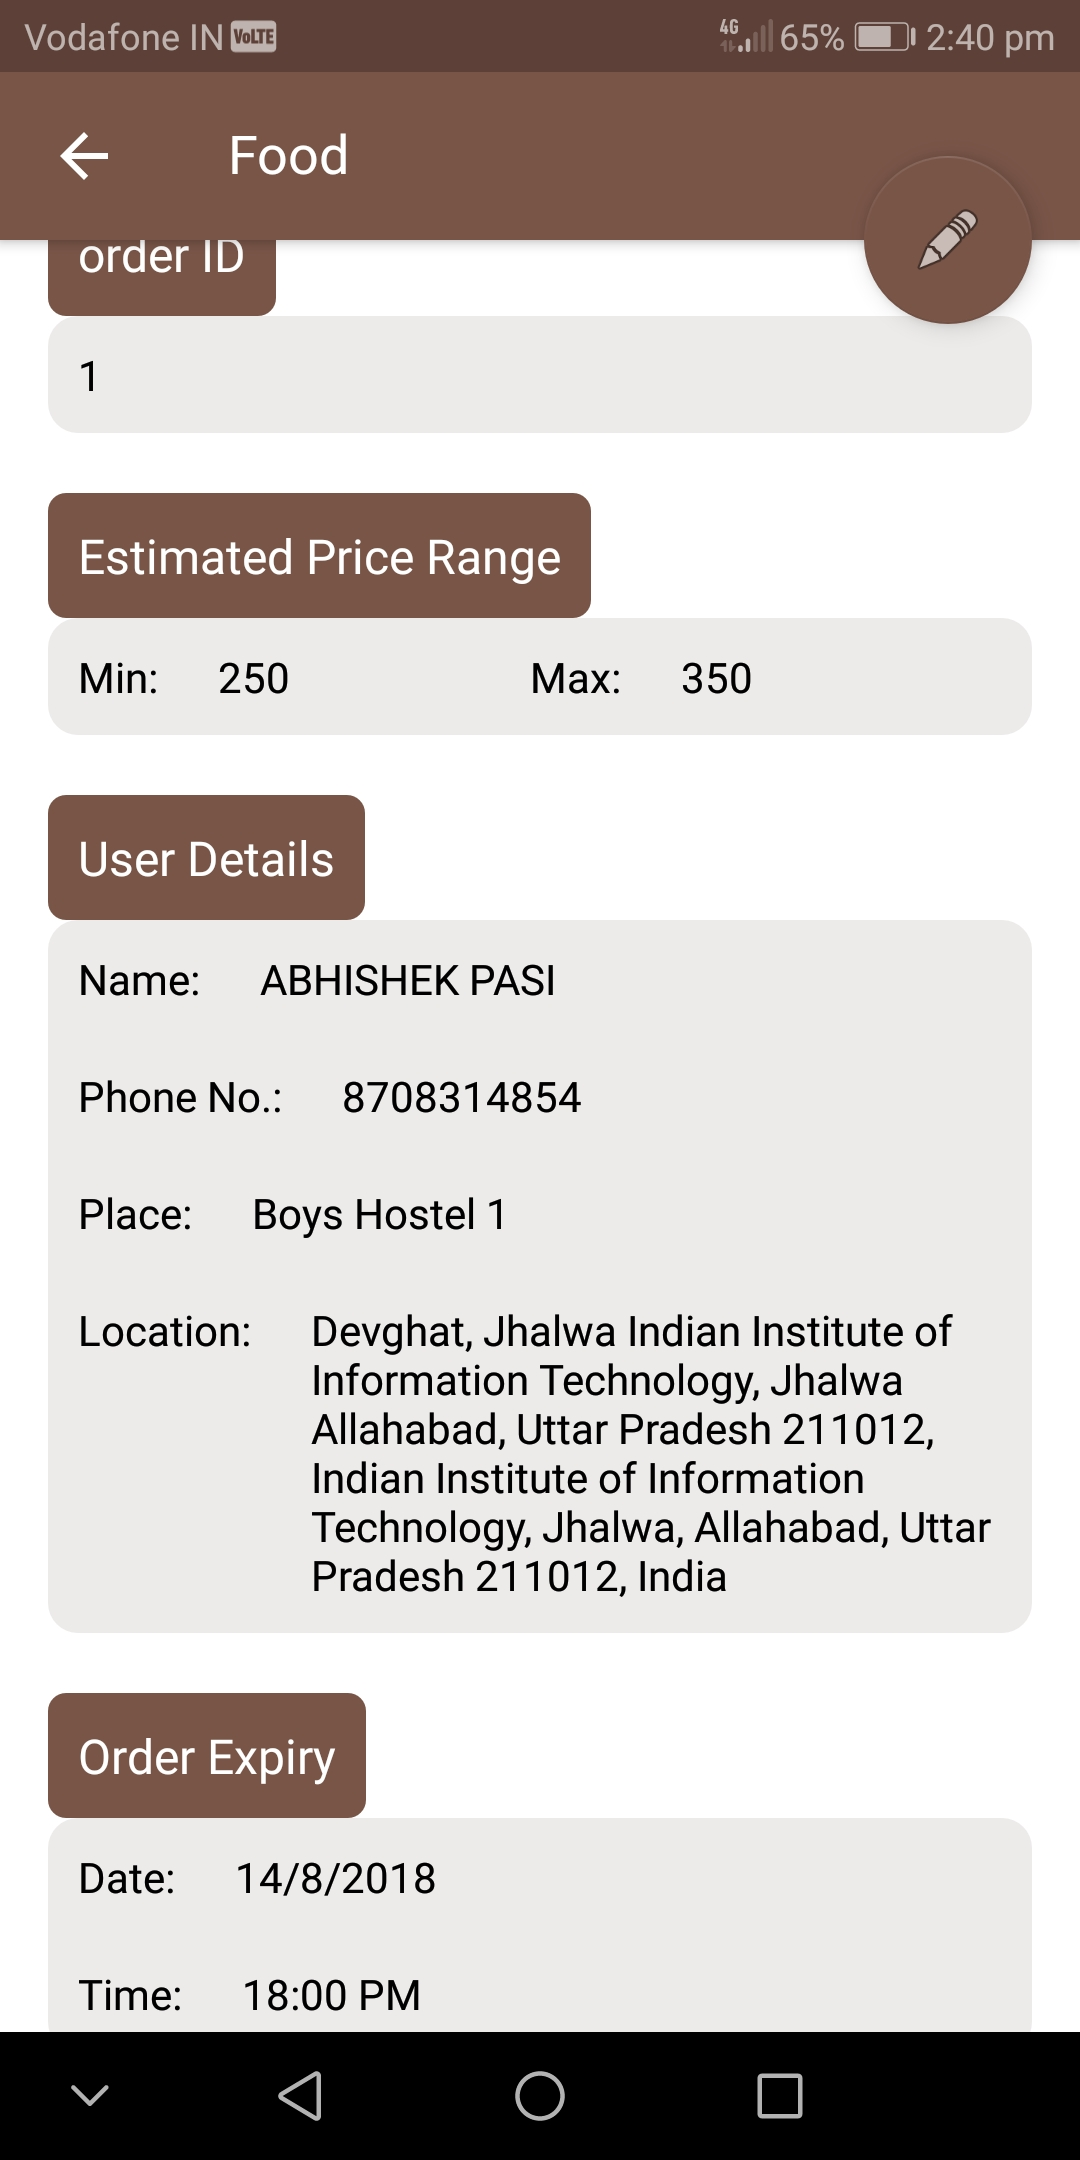
\includegraphics[width=5cm]{order_detail2.jpg}
\caption{\centering Order detail view}
\end{subfigure}
\begin{subfigure}[b]{.3\textwidth}
\centering
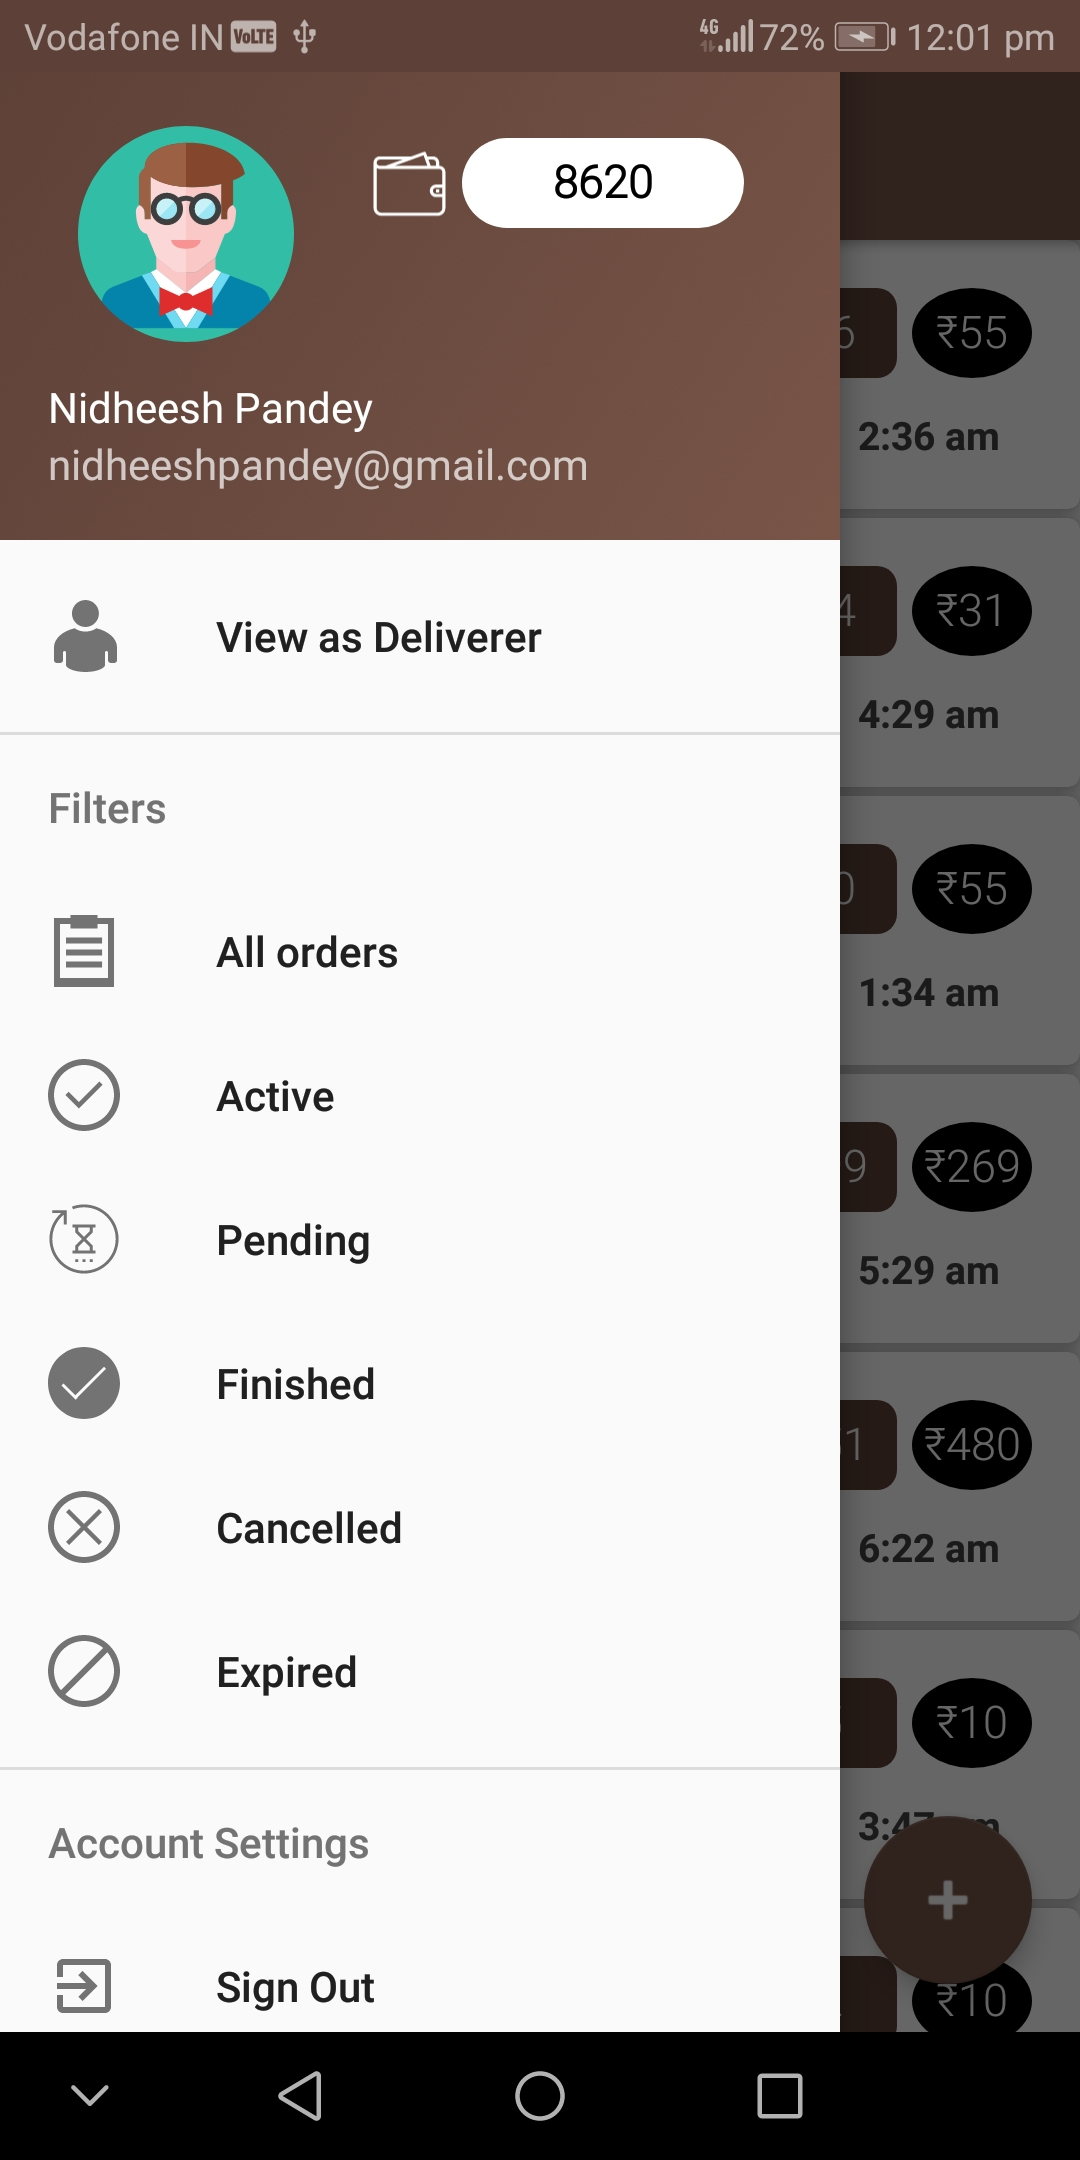
\includegraphics[width=5cm]{shopper_drawer.jpg}
\caption{\centering Shopper Navigation}
\end{subfigure}
\caption{Shopper order Detail view and Shopper Navigation drawer} 
\label{fig:NASA_Logo}
\end{figure}


\subsection{Placing New Order}
\begin{itemize}
\item Touching the PLUS Floating Action Button on the bottom right on the Shopper View screen opens up the form for placing a new order.
\item We need to give the order Description, its Category, an estimated price range.
\item We can choose to give the expiry Date and Time for that order, expiration of after which that order will automatically be removed from the global pending orders list of Deliverers.
\item We also need to set the delivery location for our order i.e the location where we want our order to be delivered. We are using Google Places API for doing this.
\item We are storing this Delivery location in our database, so that it can be used by the deliverer to track the delivery location.
\item Payment of the order is being done from the shopper’s PayTM wallet using PayTM payments SDK.
\item After successful payment and placing of order, that order is added as a card in the Recycler view in the Shopper View screen with status as PENDING.

\end{itemize}

\begin{figure}[h!]
\begin{subfigure}[h!]{.3\textwidth}
\centering
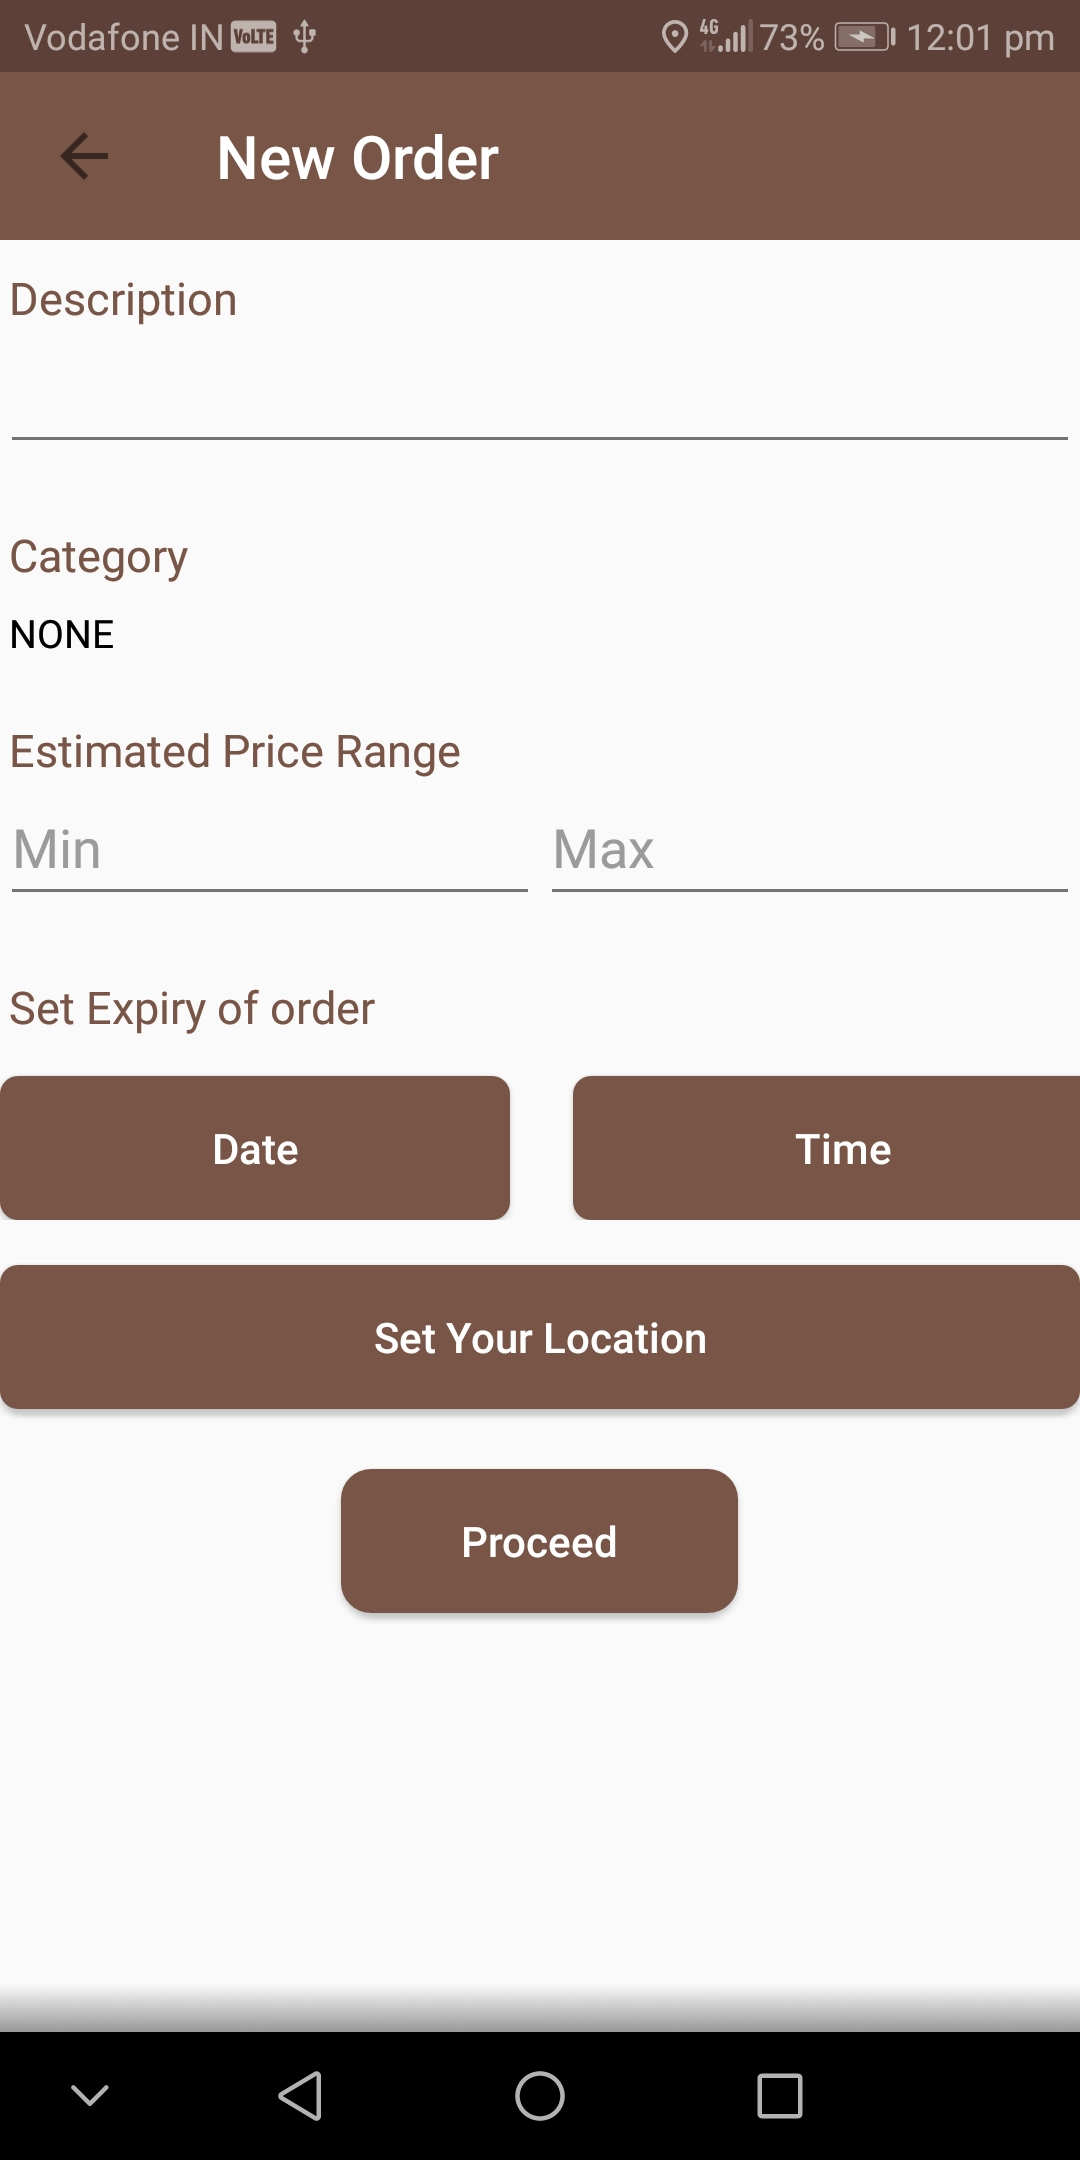
\includegraphics[width=5cm]{empty_form.jpg}
\caption{\centering New Order form}
\end{subfigure}
\begin{subfigure}[h!]{.3\textwidth}
\centering
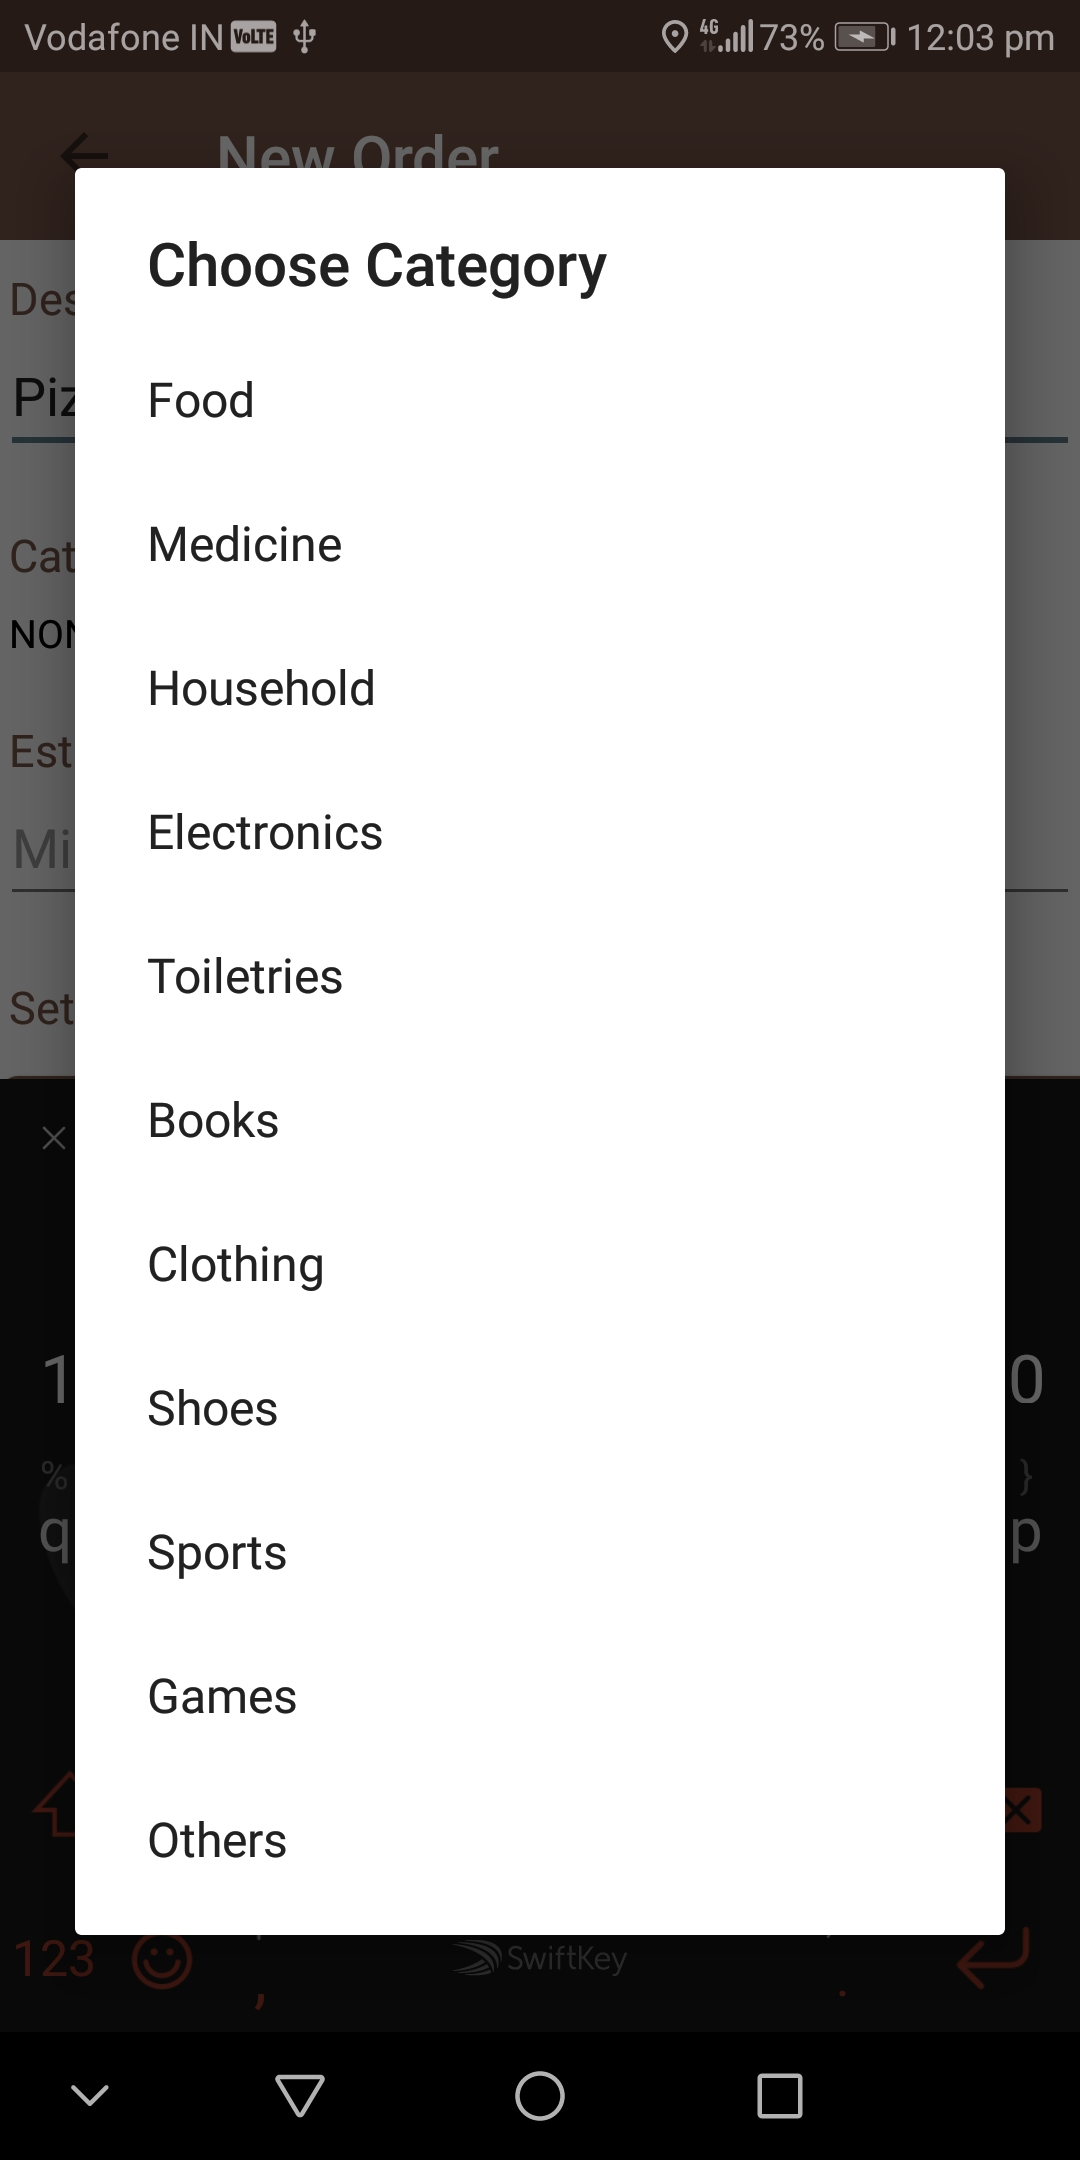
\includegraphics[width=5cm]{categories.jpg}
\caption{\centering Choosing the Category for order}
\end{subfigure}
\begin{subfigure}[h!]{.3\textwidth}
\centering
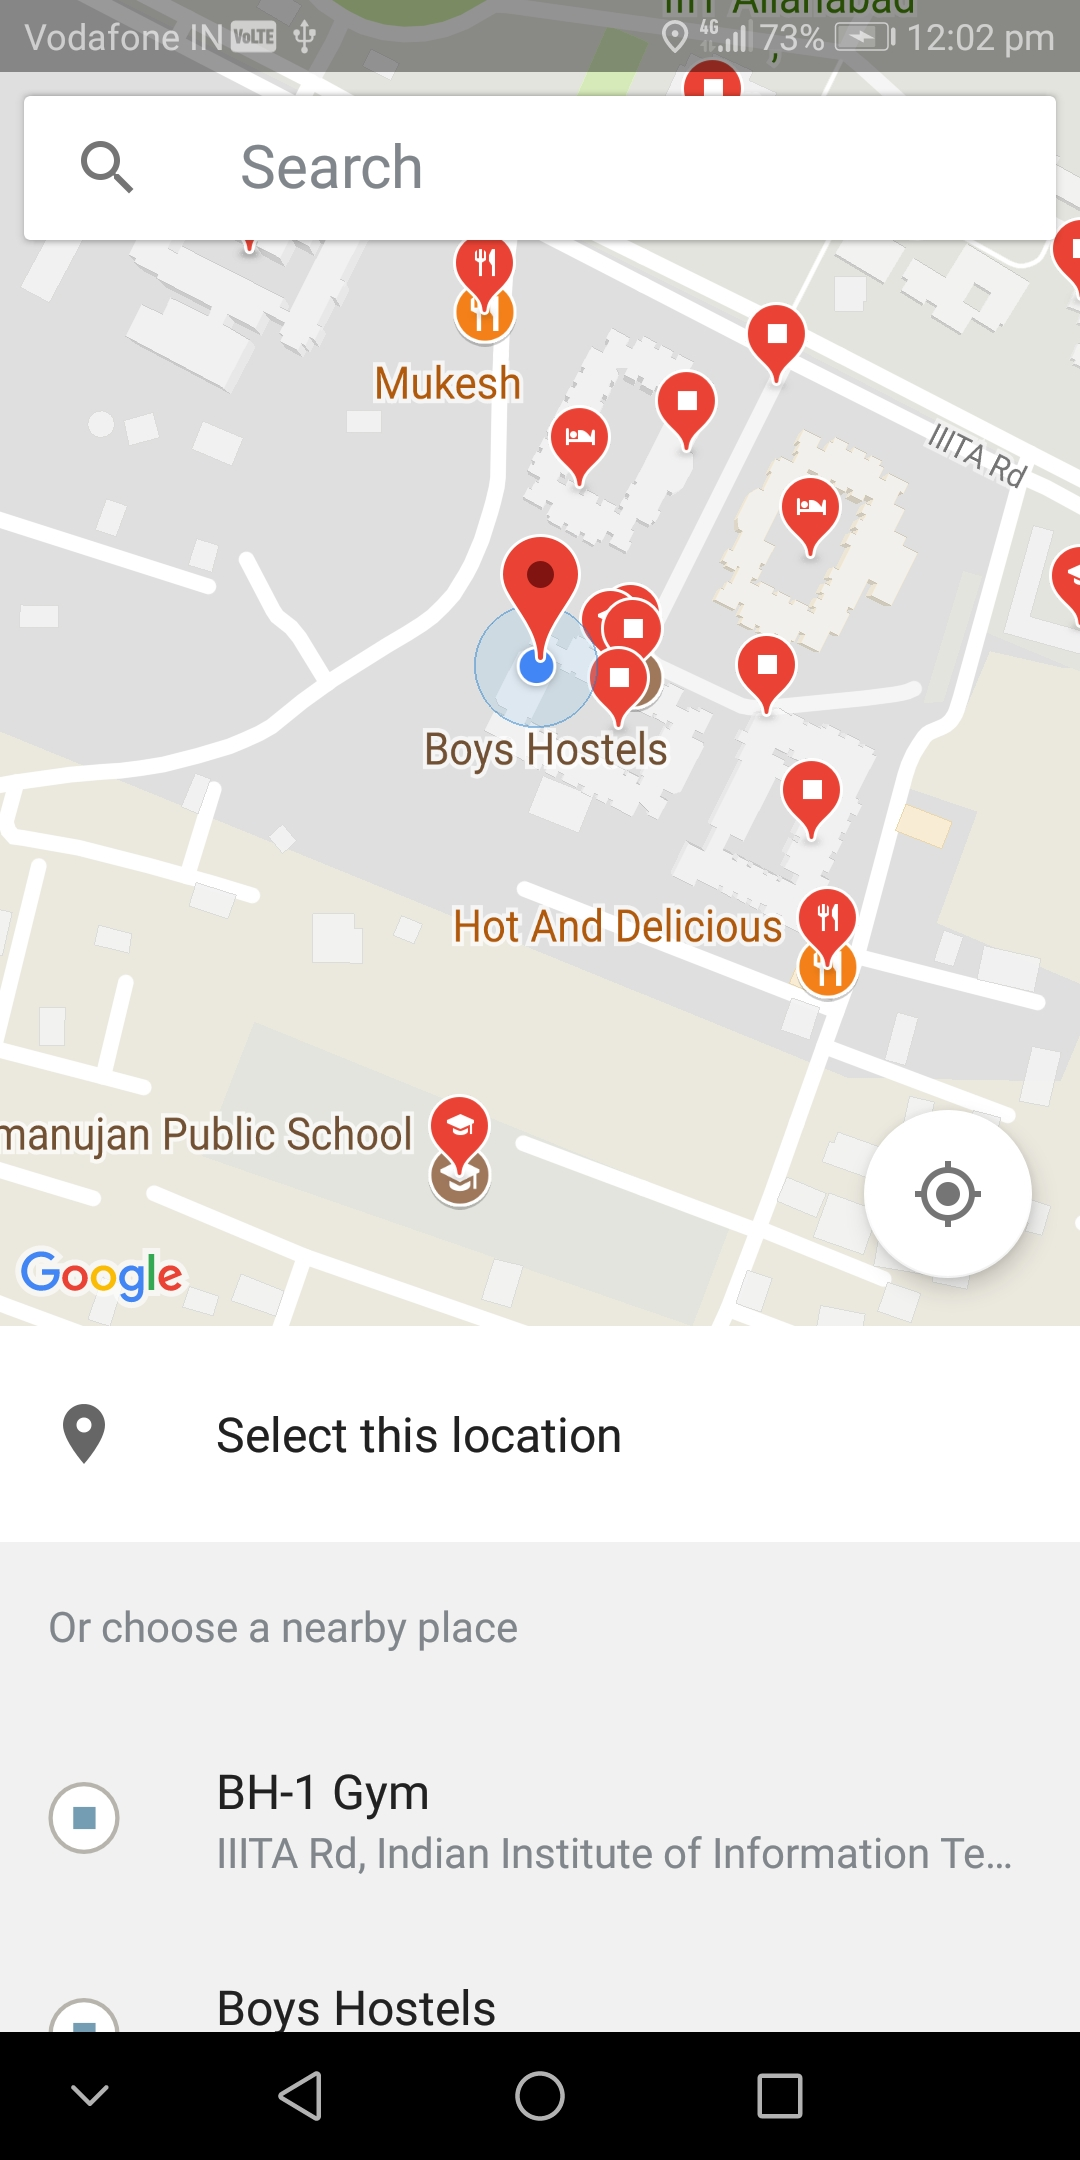
\includegraphics[width=5cm]{place_picker.jpg}
\caption{\centering Setting the delivery location for order}
\end{subfigure}

\begin{subfigure}[h!]{.3\textwidth}
\centering
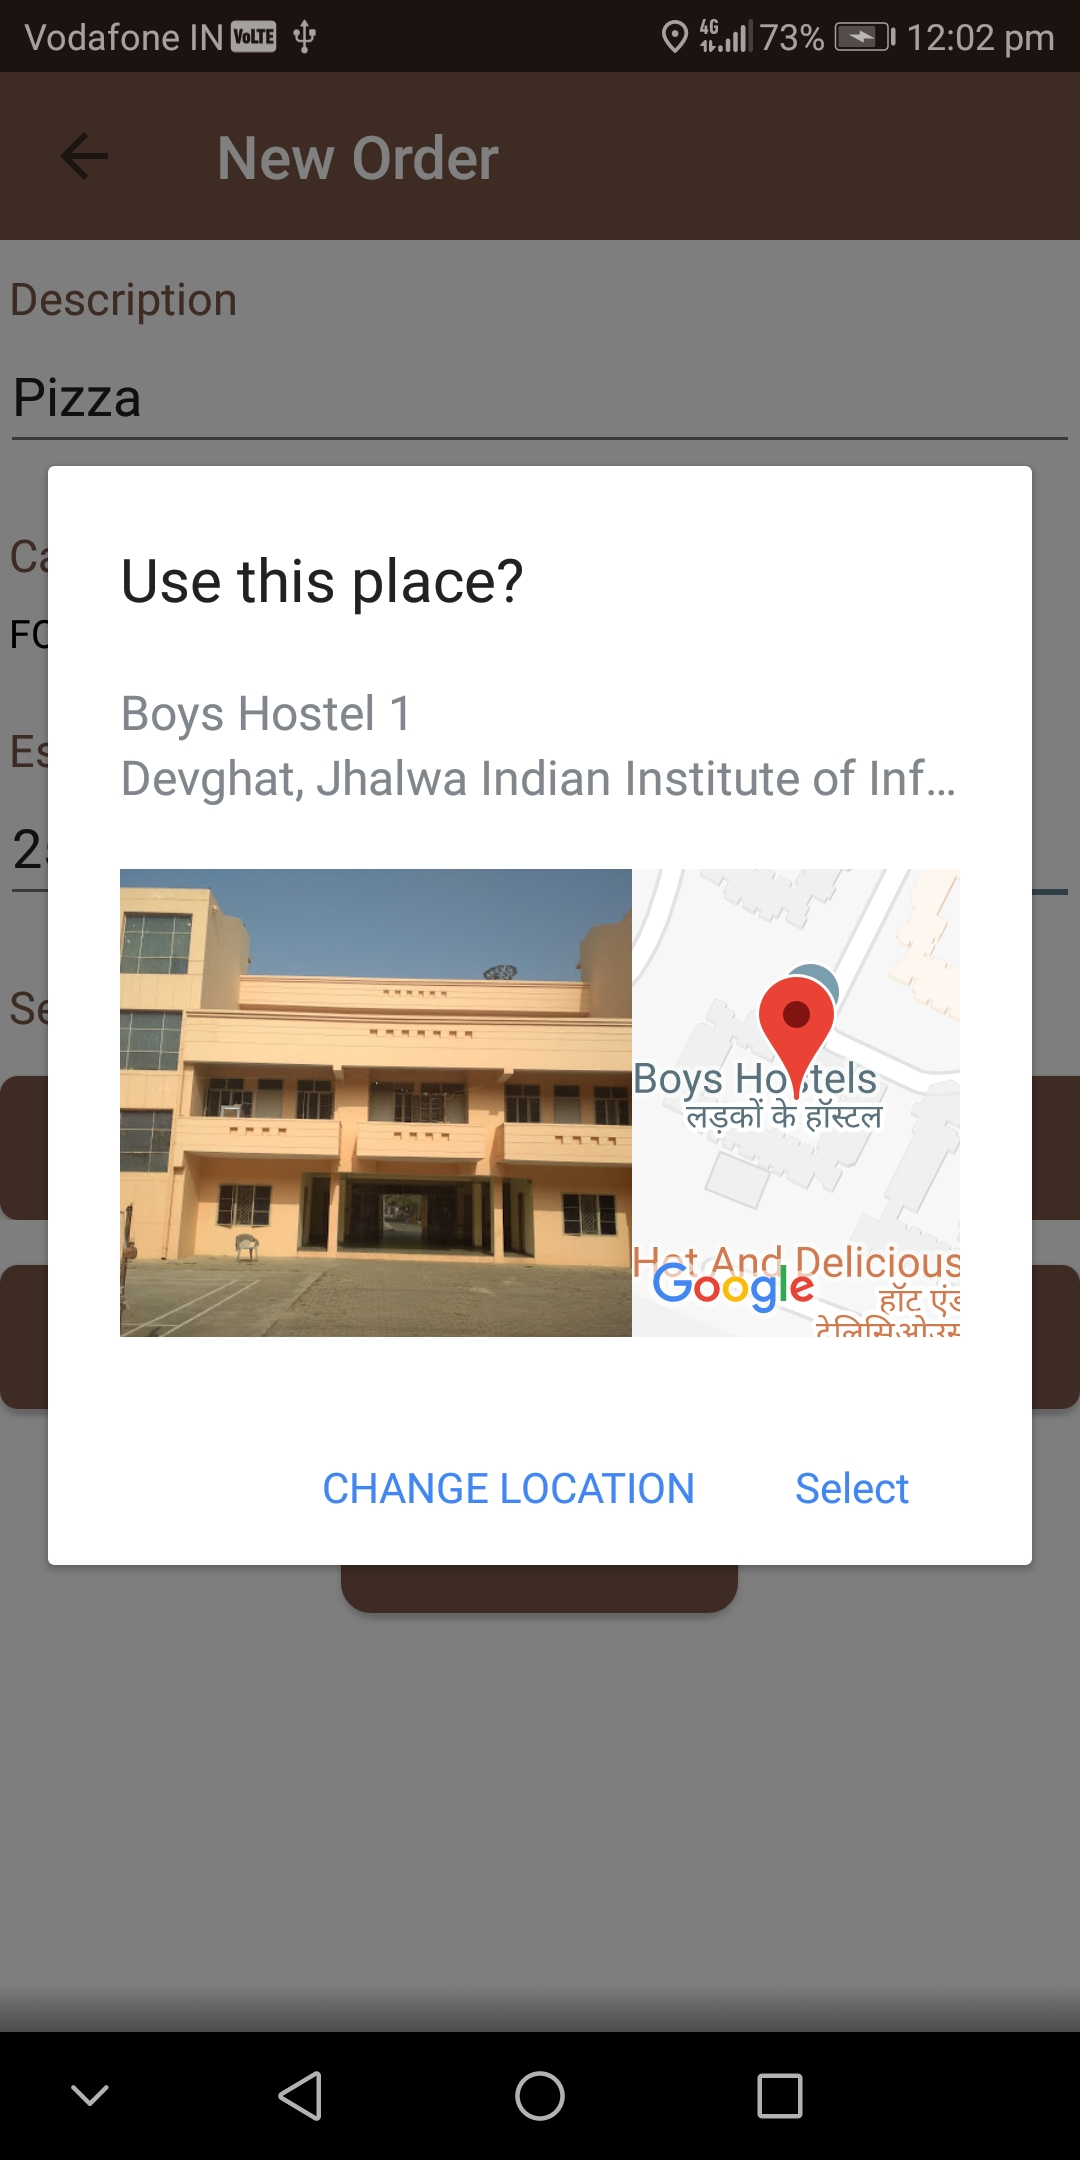
\includegraphics[width=5cm]{place.jpg}
\caption{\centering COnfirming the delivery location for order}
\end{subfigure}
\begin{subfigure}[h!]{.3\textwidth}
\centering
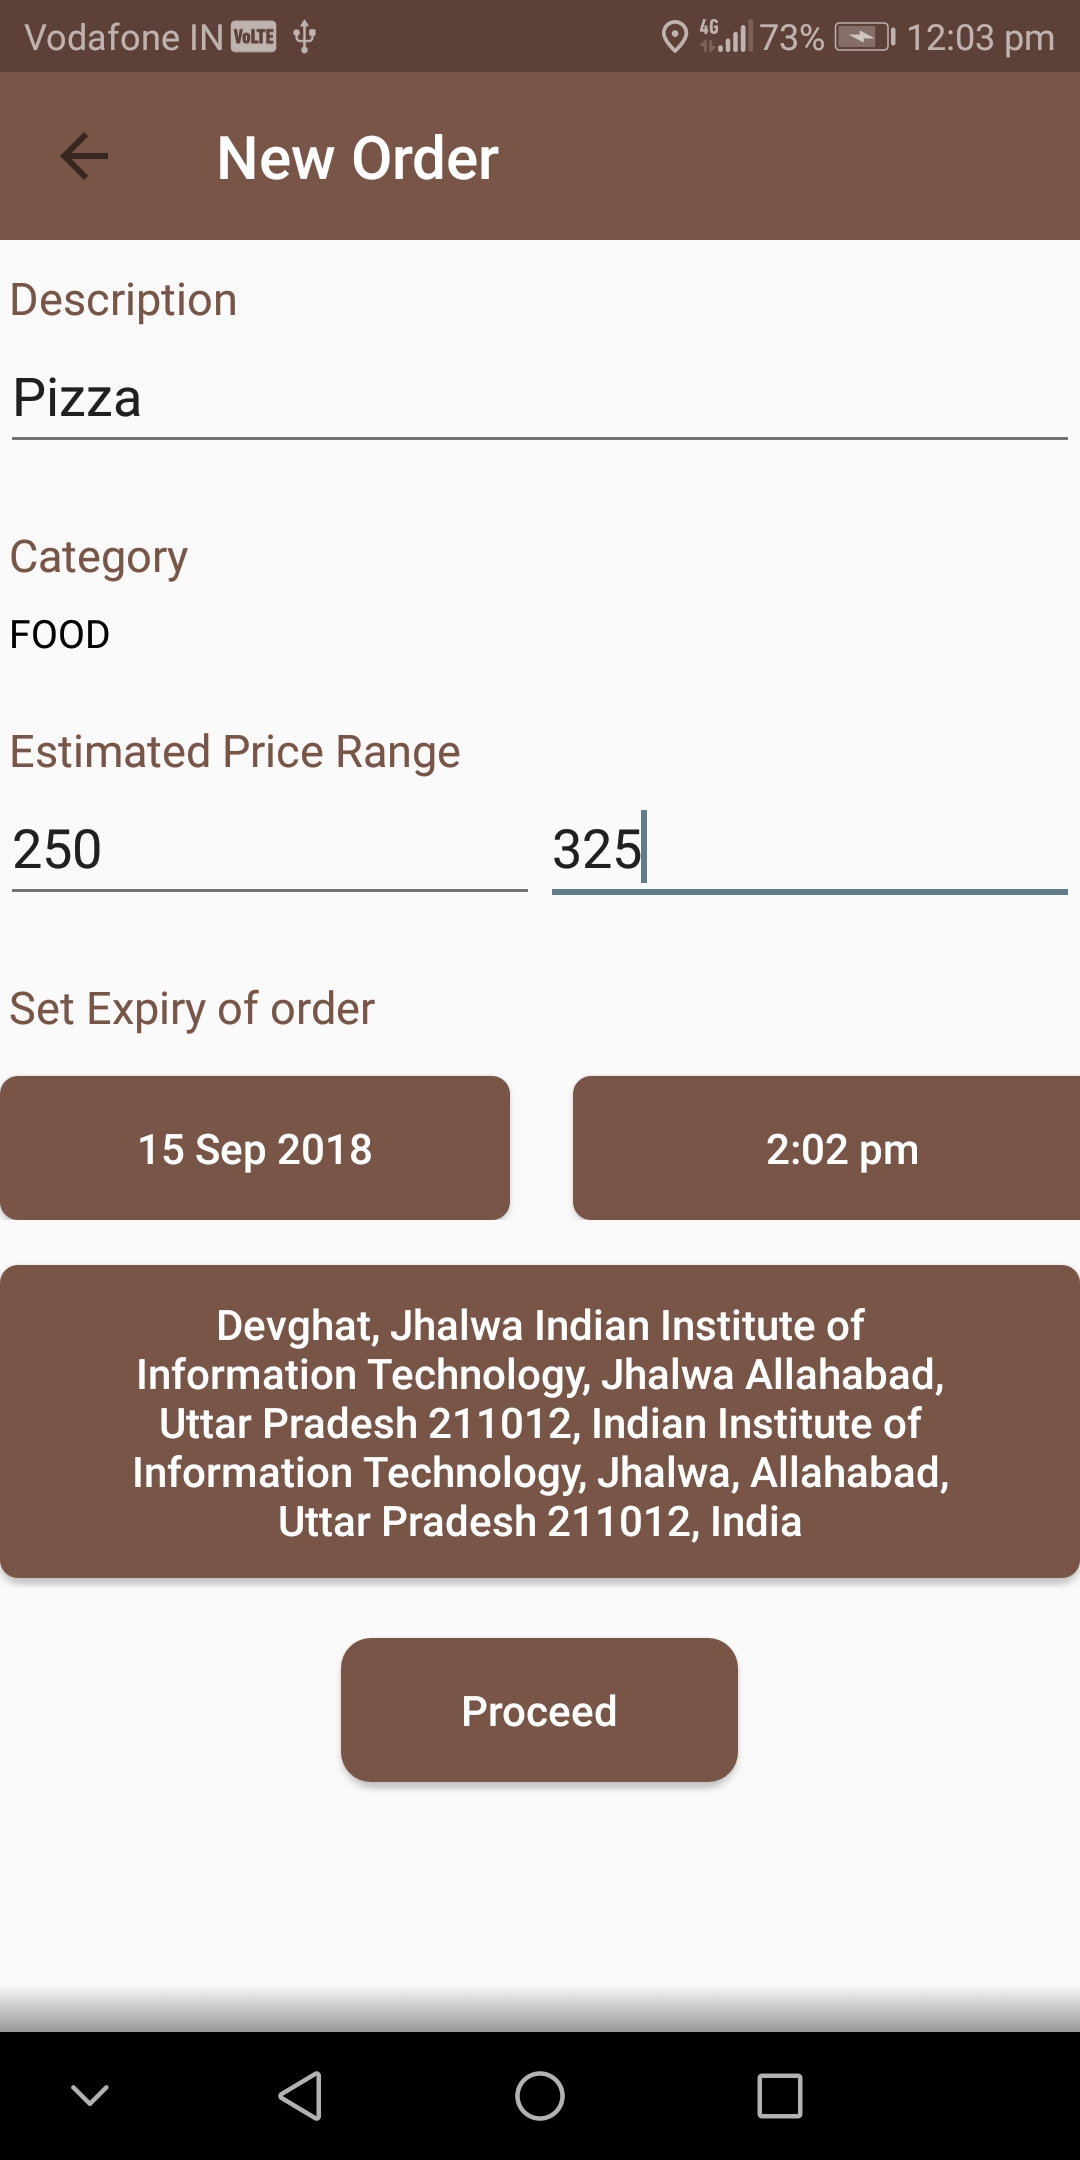
\includegraphics[width=5cm]{filled_form.jpg}
\caption{\centering Filled form}
\end{subfigure}
\begin{subfigure}[h!]{.3\textwidth}
\centering
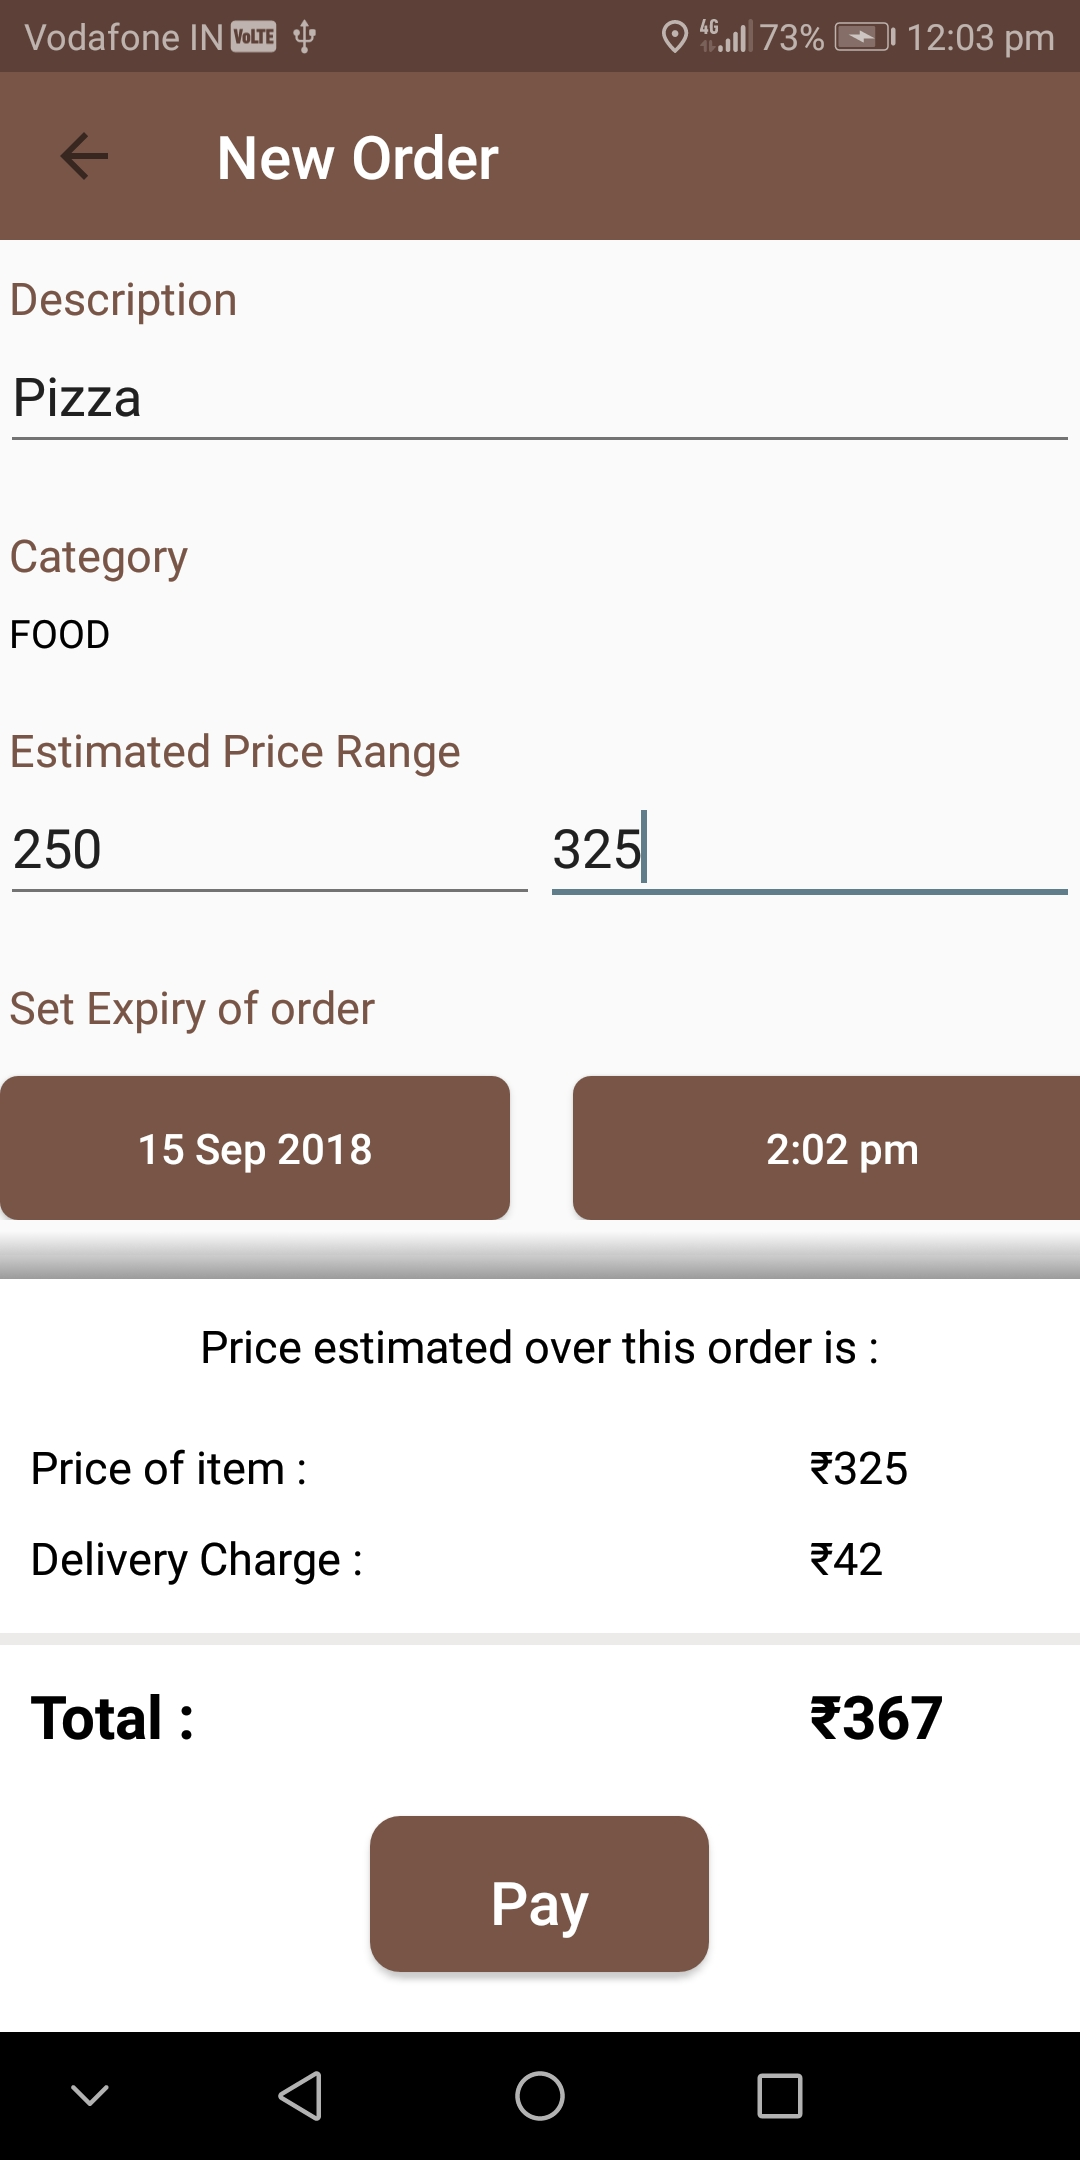
\includegraphics[width=5cm]{pay.jpg}
\caption{\centering Order Price display using Bottomsheet}
\end{subfigure}
\caption{Placing new order} 
\label{fig:NASA_Logo}
\end{figure}


\begin{figure}[h!]
\begin{subfigure}[h!]{.3\textwidth}
\centering
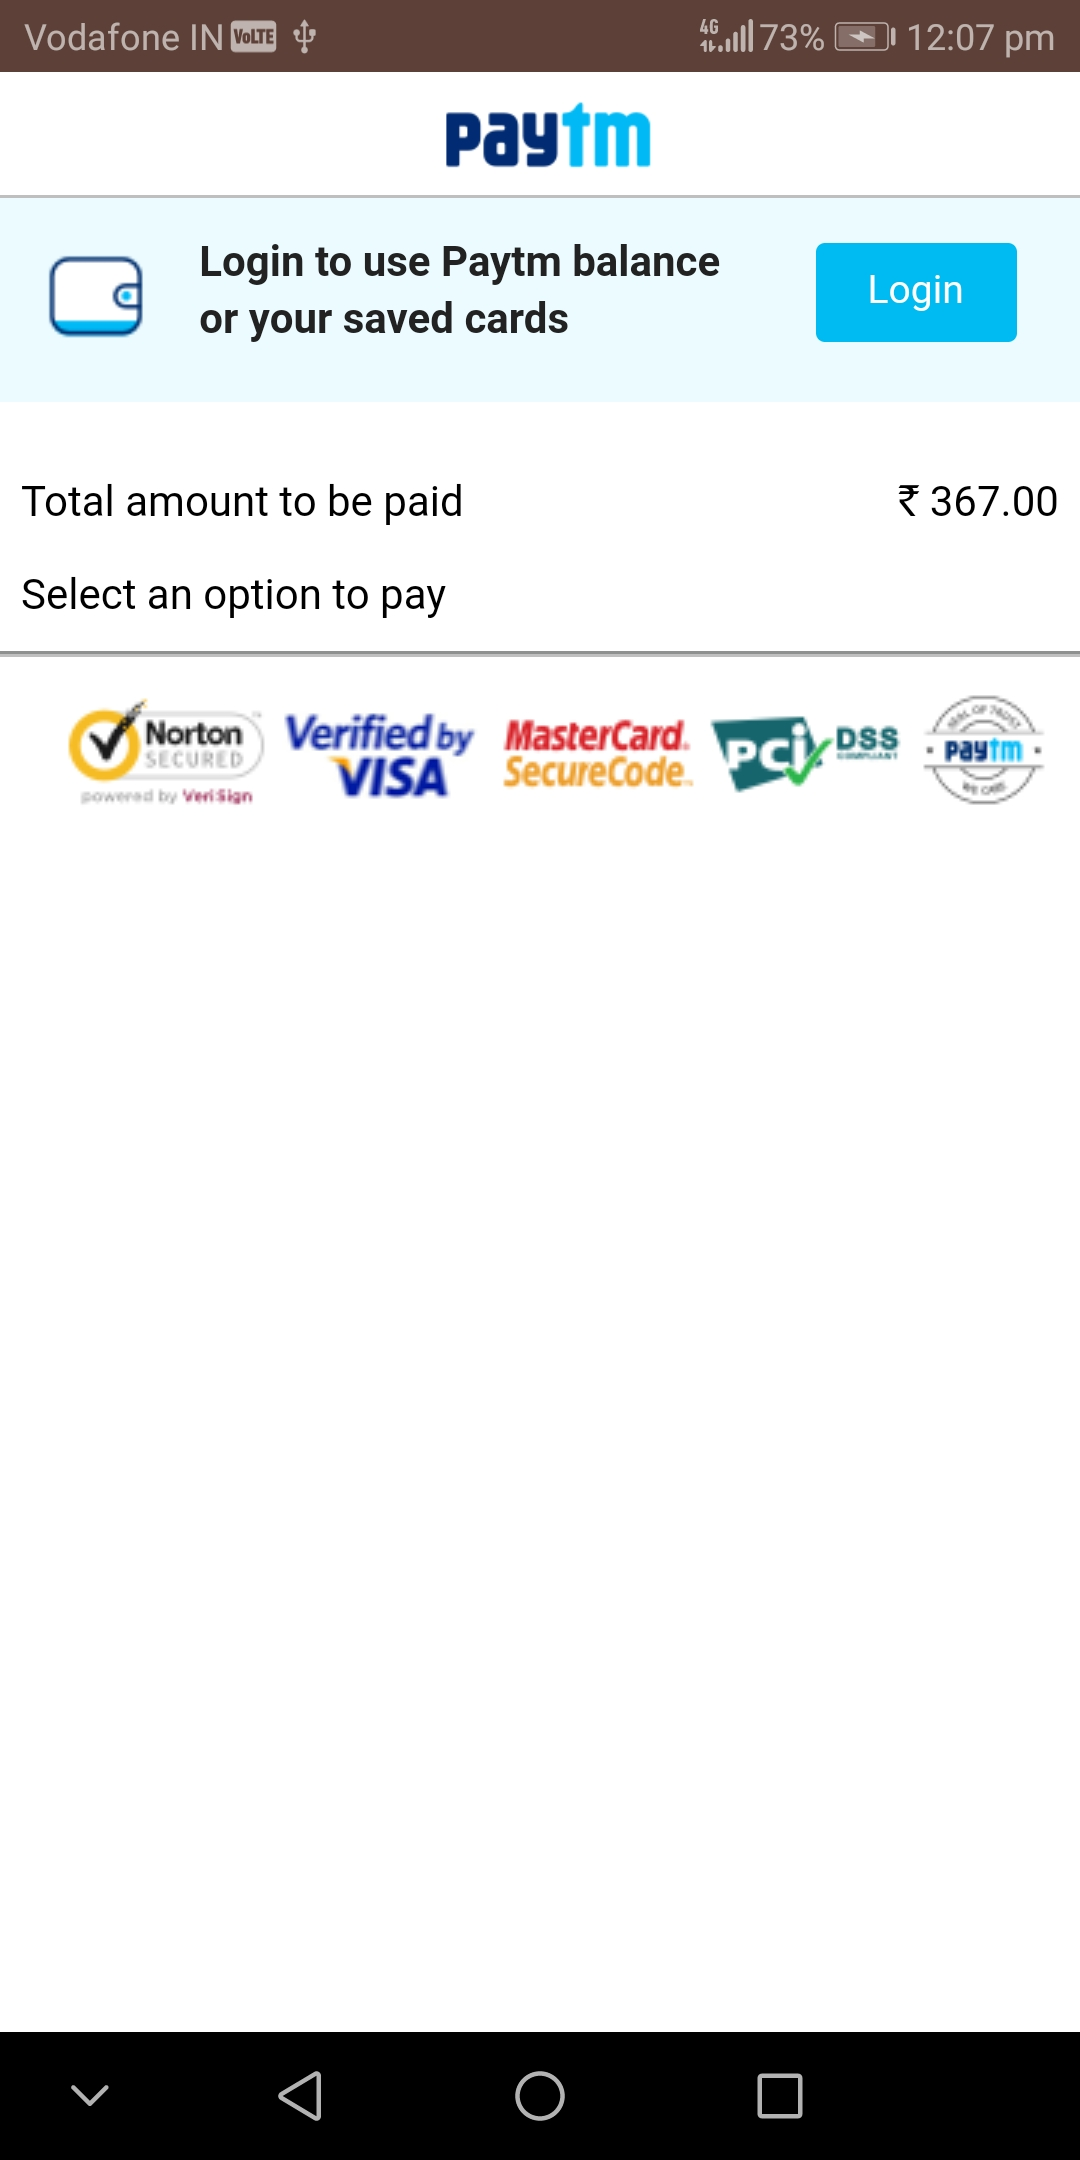
\includegraphics[width=5cm]{paytm_start.jpg}
\caption{\centering Login to Paytm to pay}
\end{subfigure}
\begin{subfigure}[h!]{.3\textwidth}
\centering
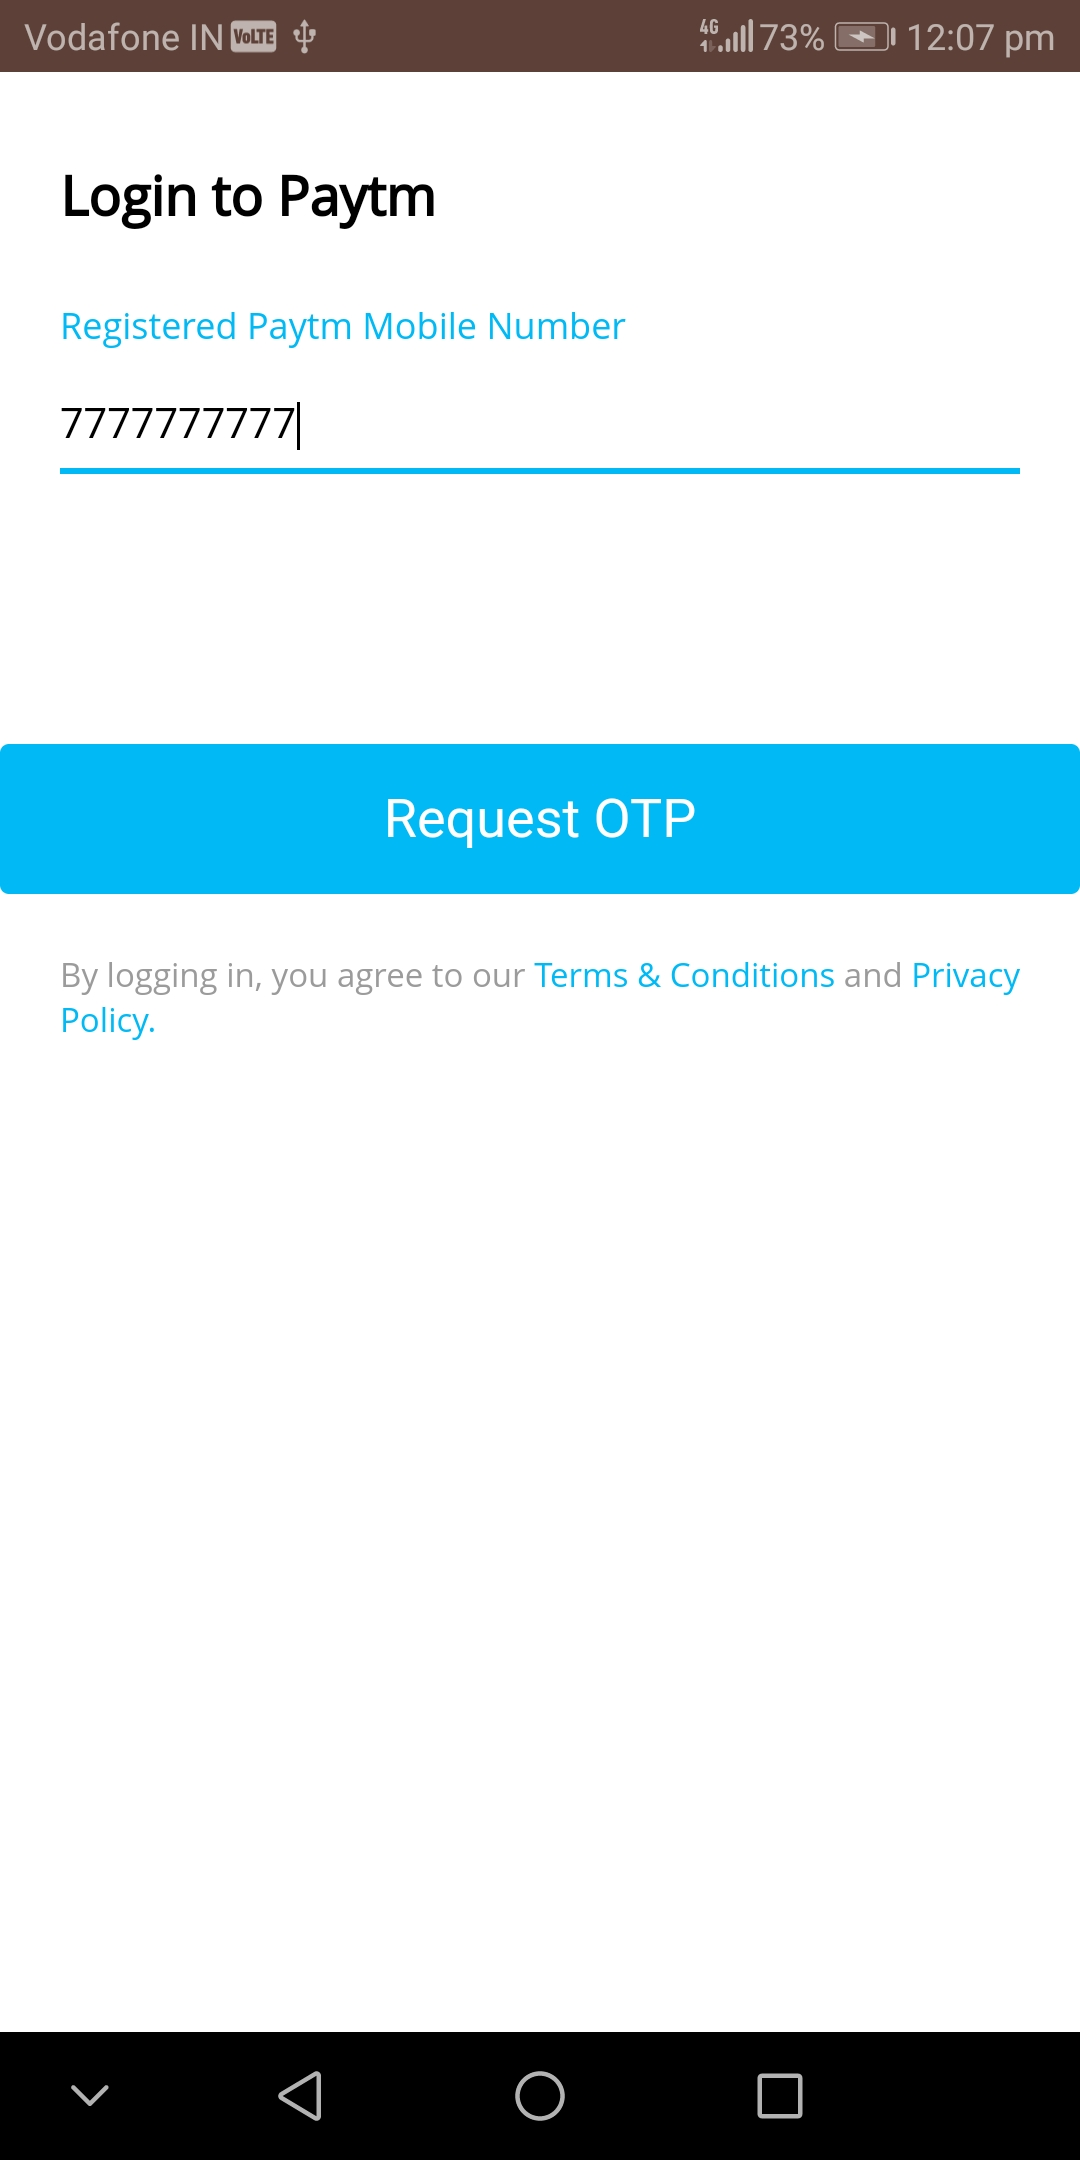
\includegraphics[width=5cm]{mobile_number.jpg}
\caption{\centering Enter the staging mobile no.}
\end{subfigure}
\begin{subfigure}[h!]{.3\textwidth}
\centering
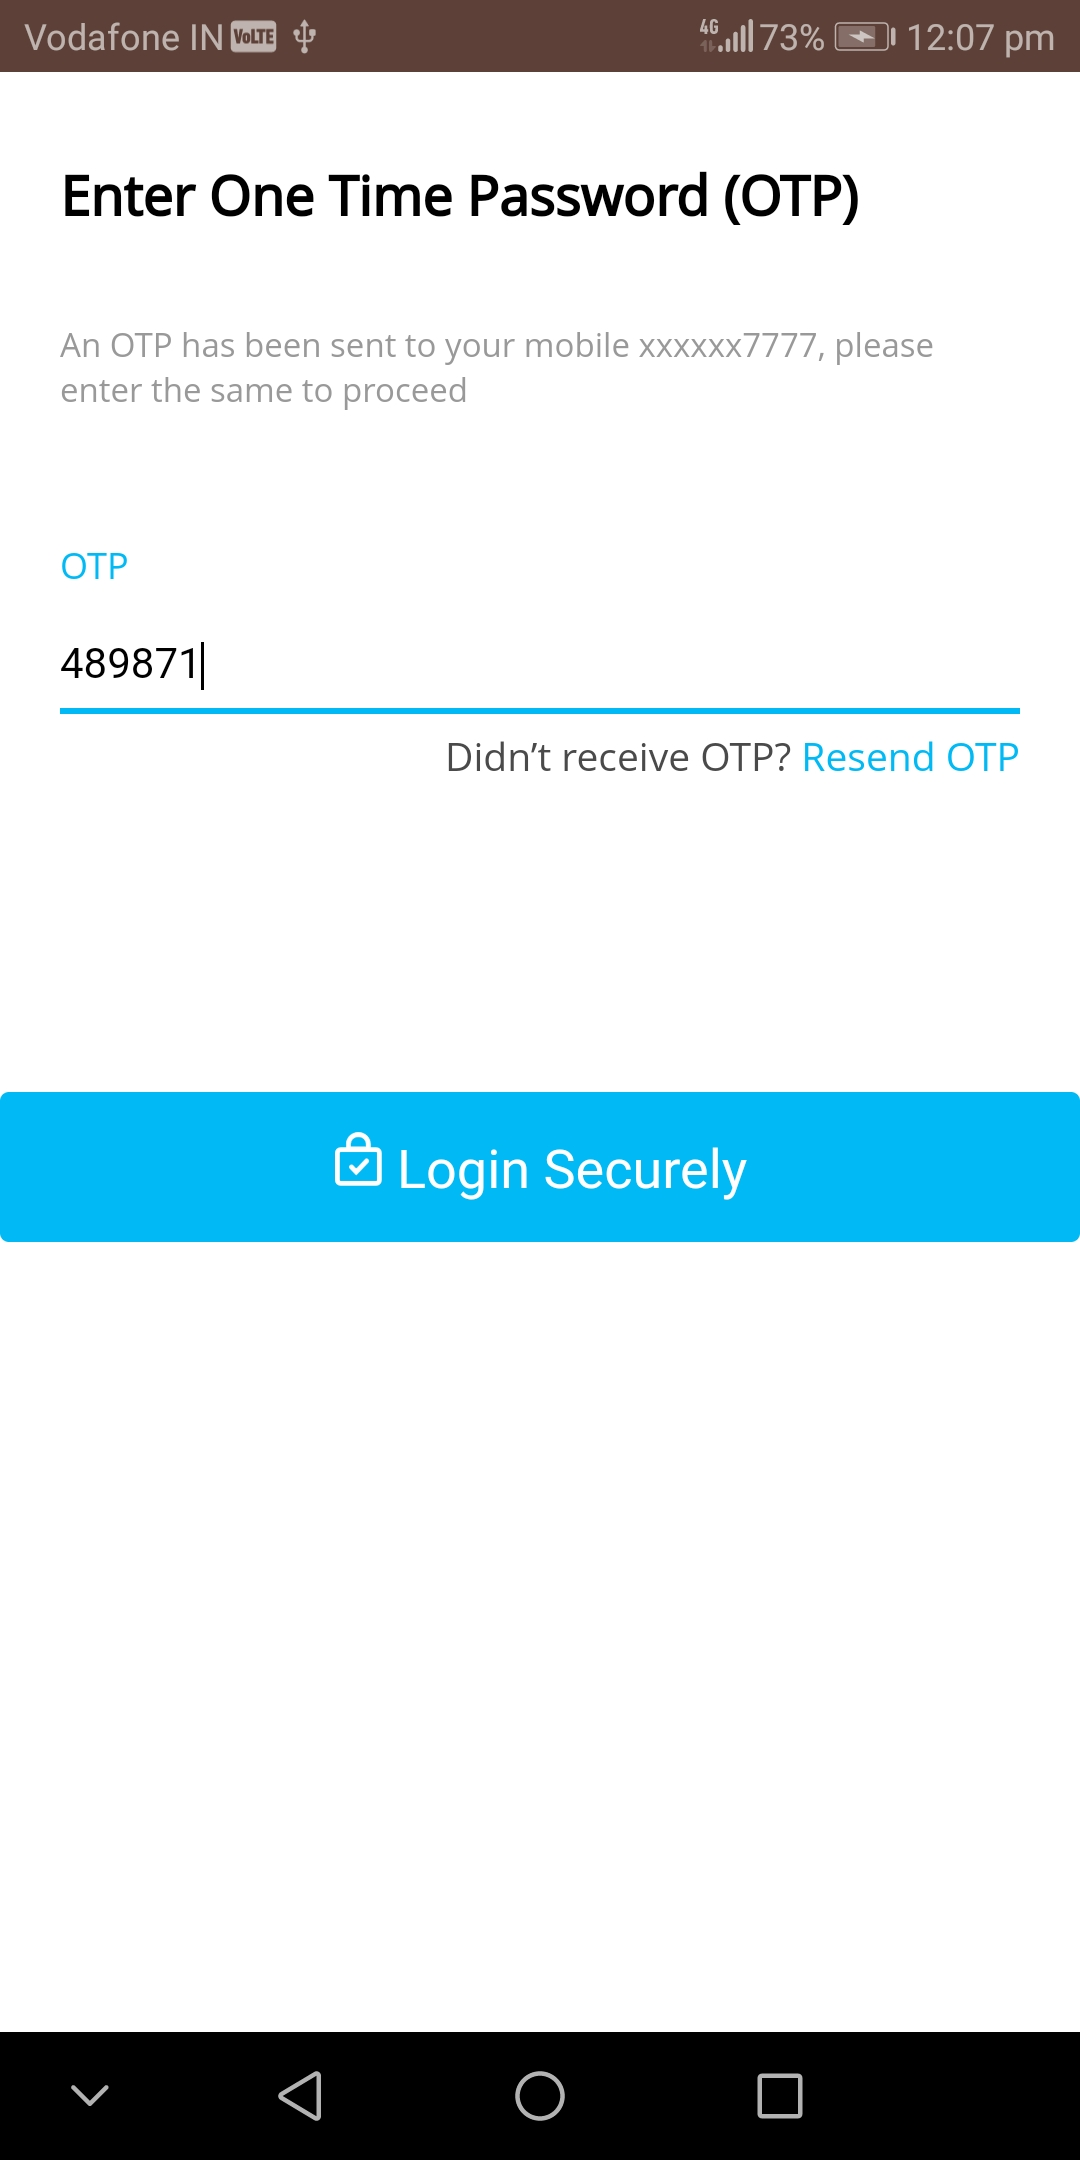
\includegraphics[width=5cm]{paytm_otp.jpg}
\caption{\centering Enter the staging OTP}
\end{subfigure}

\begin{subfigure}[h!]{.3\textwidth}
\centering
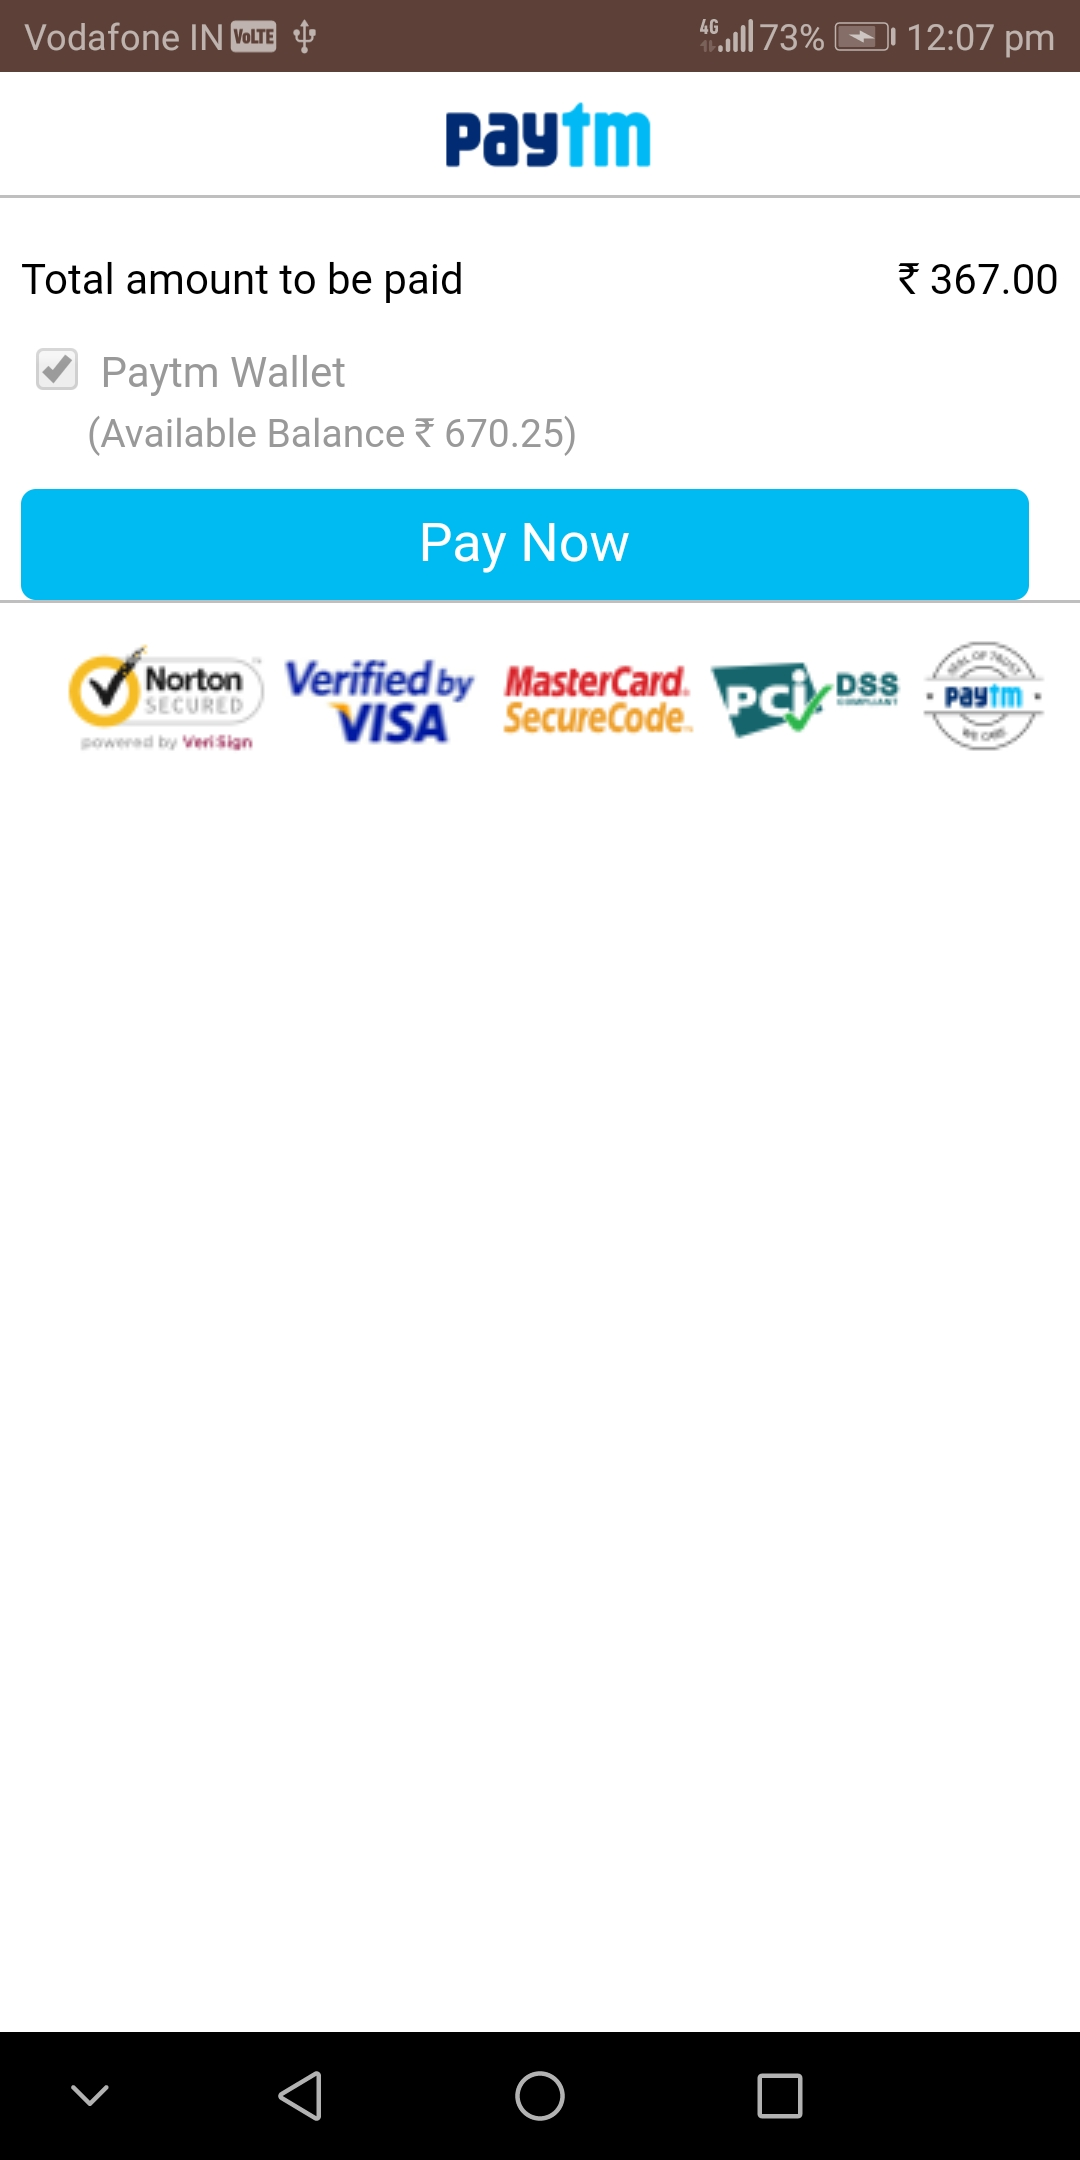
\includegraphics[width=5cm]{paytm_pay.jpg}
\caption{\centering Paying for the order using Paytm wallet}
\end{subfigure}
\begin{subfigure}[h!]{.3\textwidth}
\centering
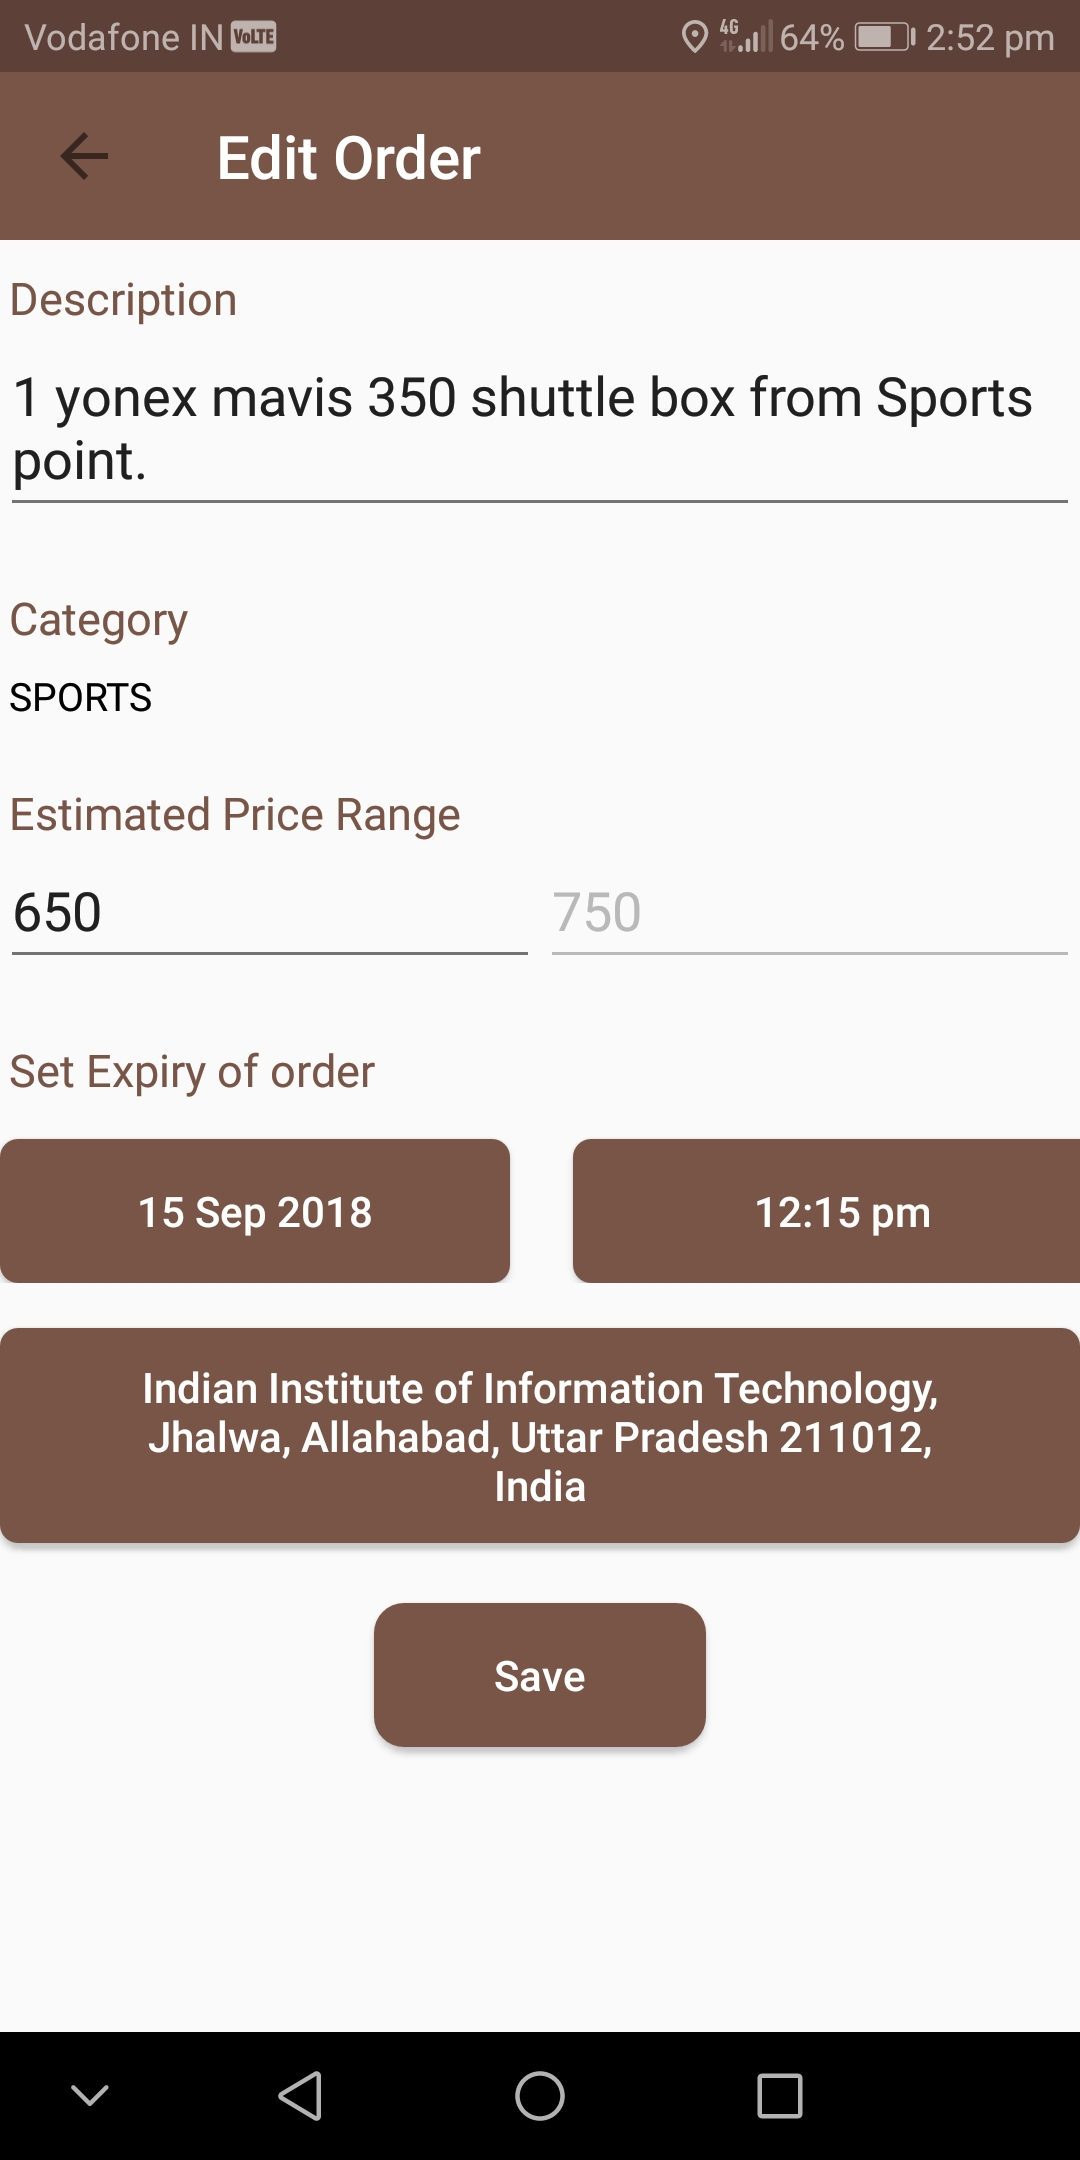
\includegraphics[width=5cm]{edit_order.jpg}
\caption{\centering Edit order form}
\end{subfigure}
\caption{Payment of order and Editing of order} 
\label{fig:NASA_Logo}
\end{figure}
\pagebreak
\pagebreak
\subsection{Editing an Order}

\begin{itemize}
\item On touching the EDIT floating Action Button on the top right of the Shopper Order Detail View screen, an edit form will be opened for that order using which we can edit the details of that order.
\end{itemize}

\subsection{Deliverer View}
\begin{itemize}
\item This screen is just like the Shopper View but according to a Deliverer.
\item You can only see the PENDING orders of the shoppers who are in the same city as yours.
\item Along with pending orders of the shoppers of your city, the default filter shows all of your Active orders, i.e. the order which you have accepted to deliver.
\item For Accepting an order from the pending orders, you have to open the order\textquotesingle s detailed view by touching the card for that order.
\end{itemize}

\subsection{Deliverer Navigation Drawer}
\begin{itemize}
\item Along with your basic profile information, wallet info. , filters and Sign-out option, here, the Navigation Drawer also displays your current location (city).
\end{itemize}

\begin{figure}[h!]
\begin{subfigure}[h!]{.24\textwidth}
\centering
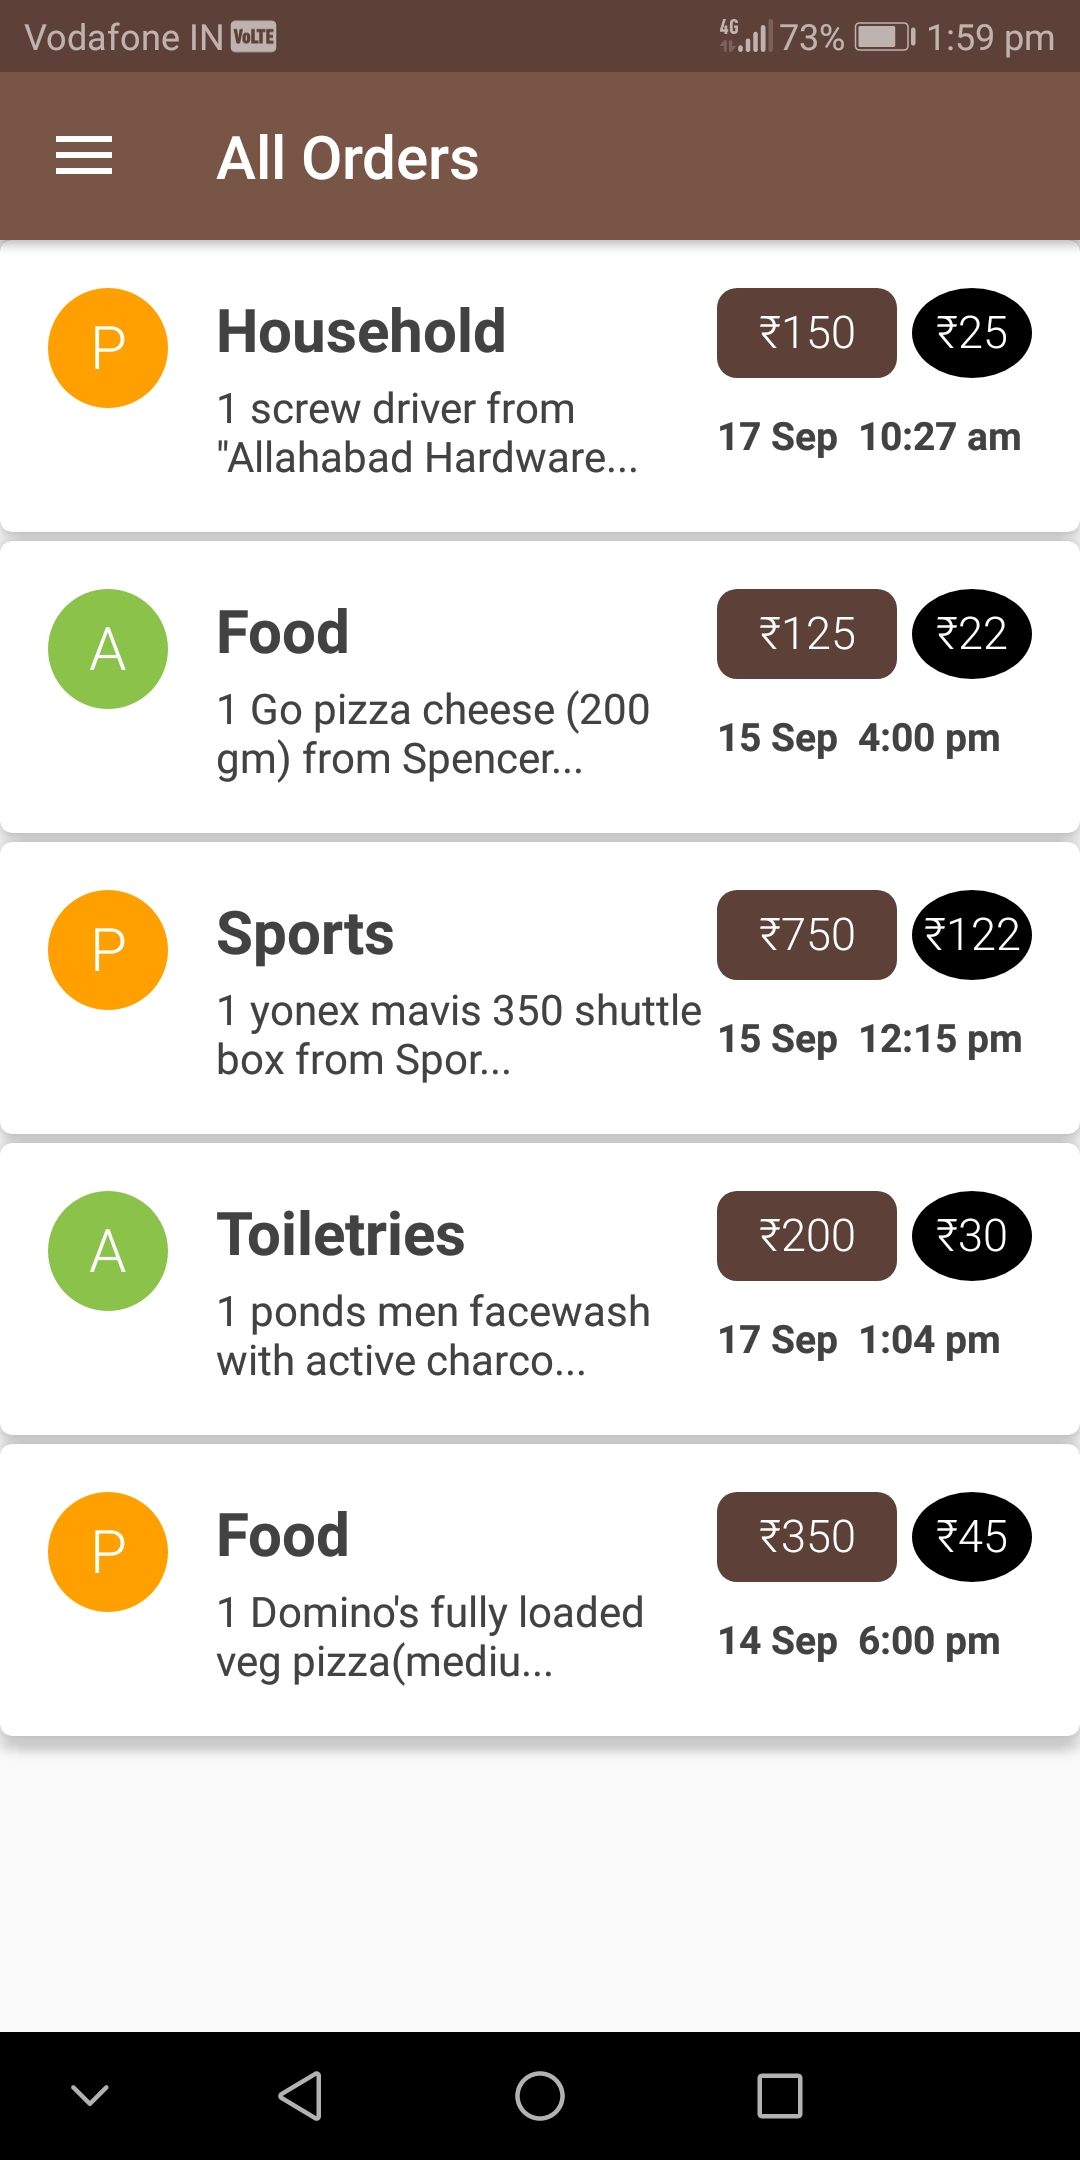
\includegraphics[width=4cm]{deliverer_view.jpg}
\caption{\centering Deliverer order view}
\end{subfigure}
\begin{subfigure}[h!]{.24\textwidth}
\centering
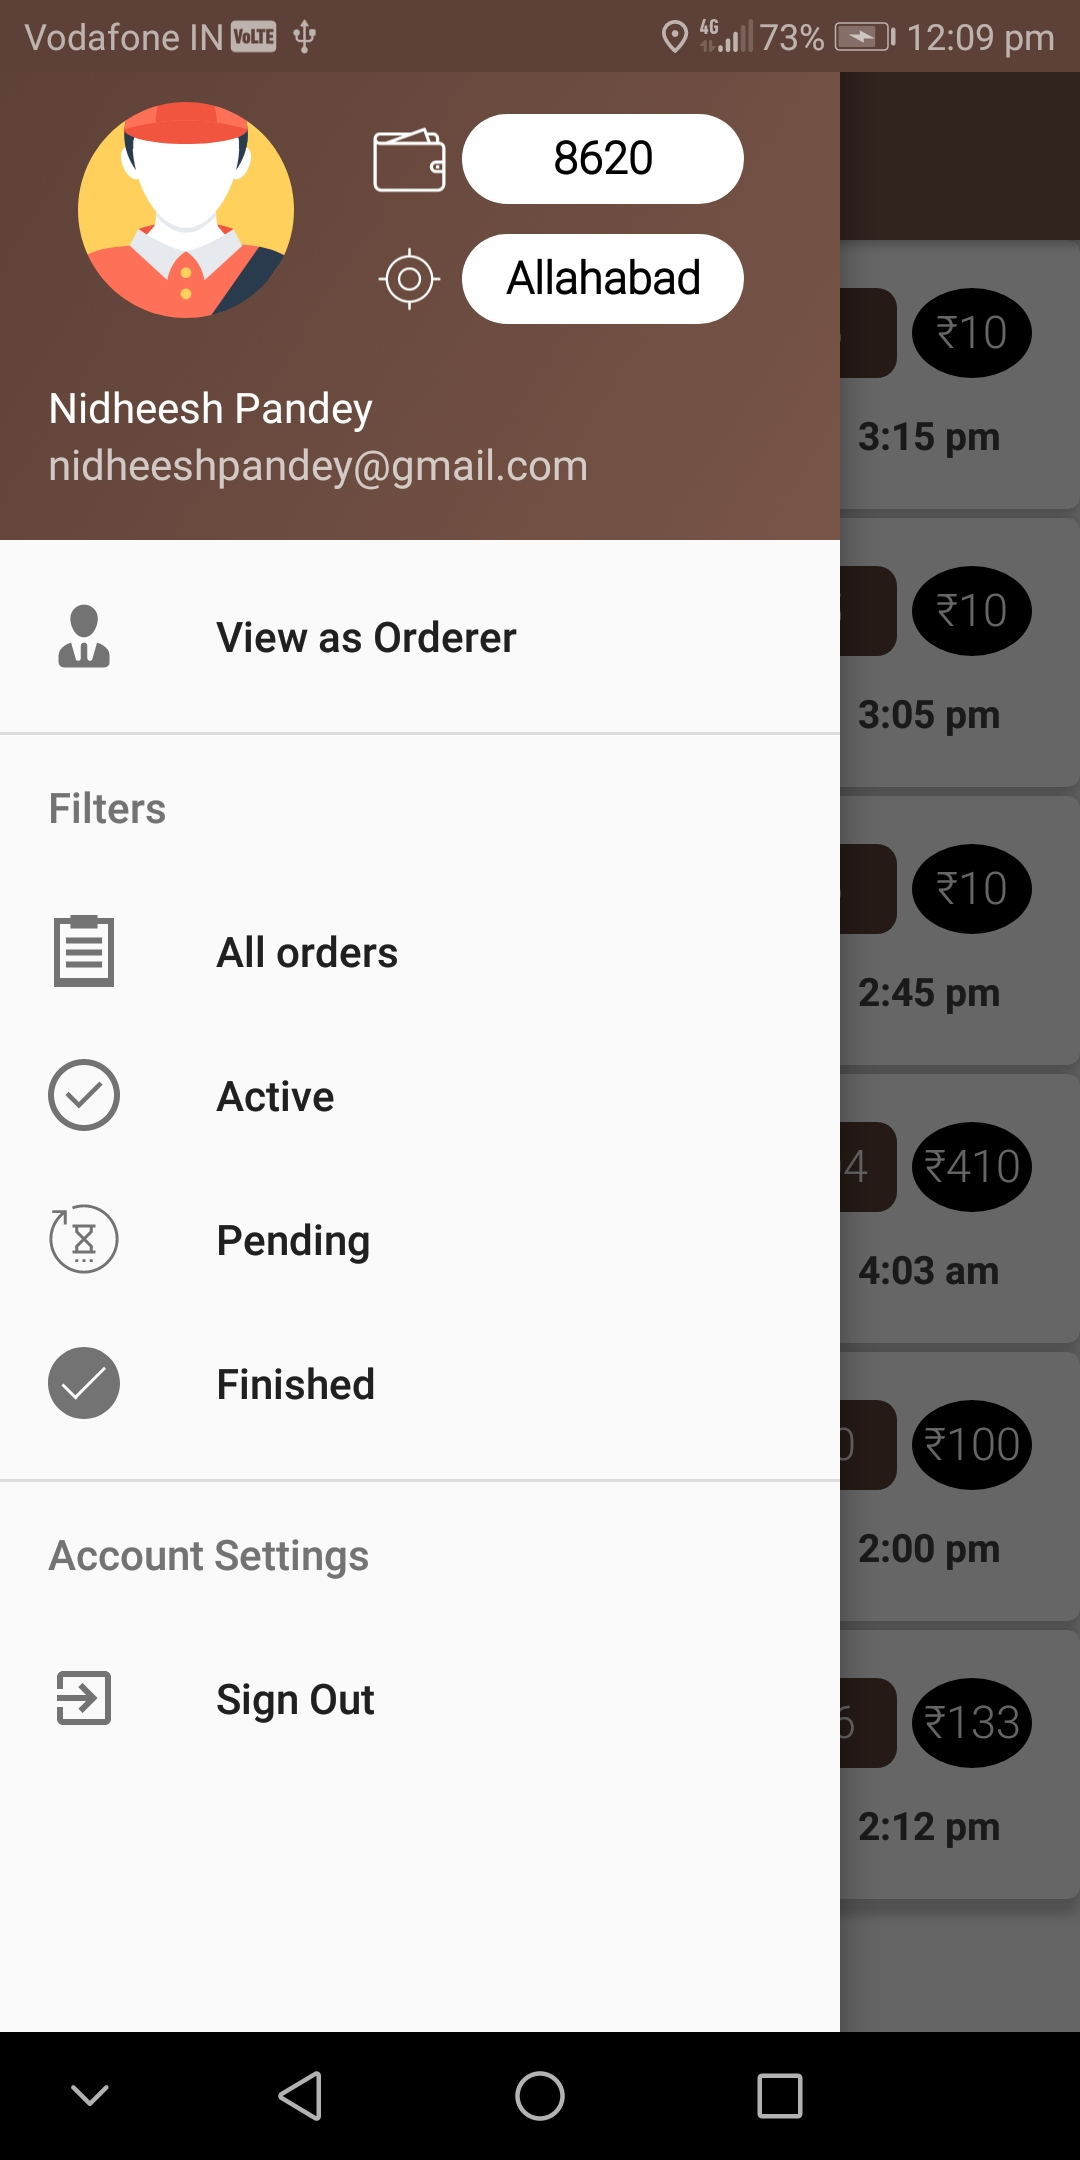
\includegraphics[width=4cm]{deliverer_drawer.jpg}
\caption{\centering Deliverer Navigation drawer}
\end{subfigure}
\begin{subfigure}[h!]{.24\textwidth}
\centering
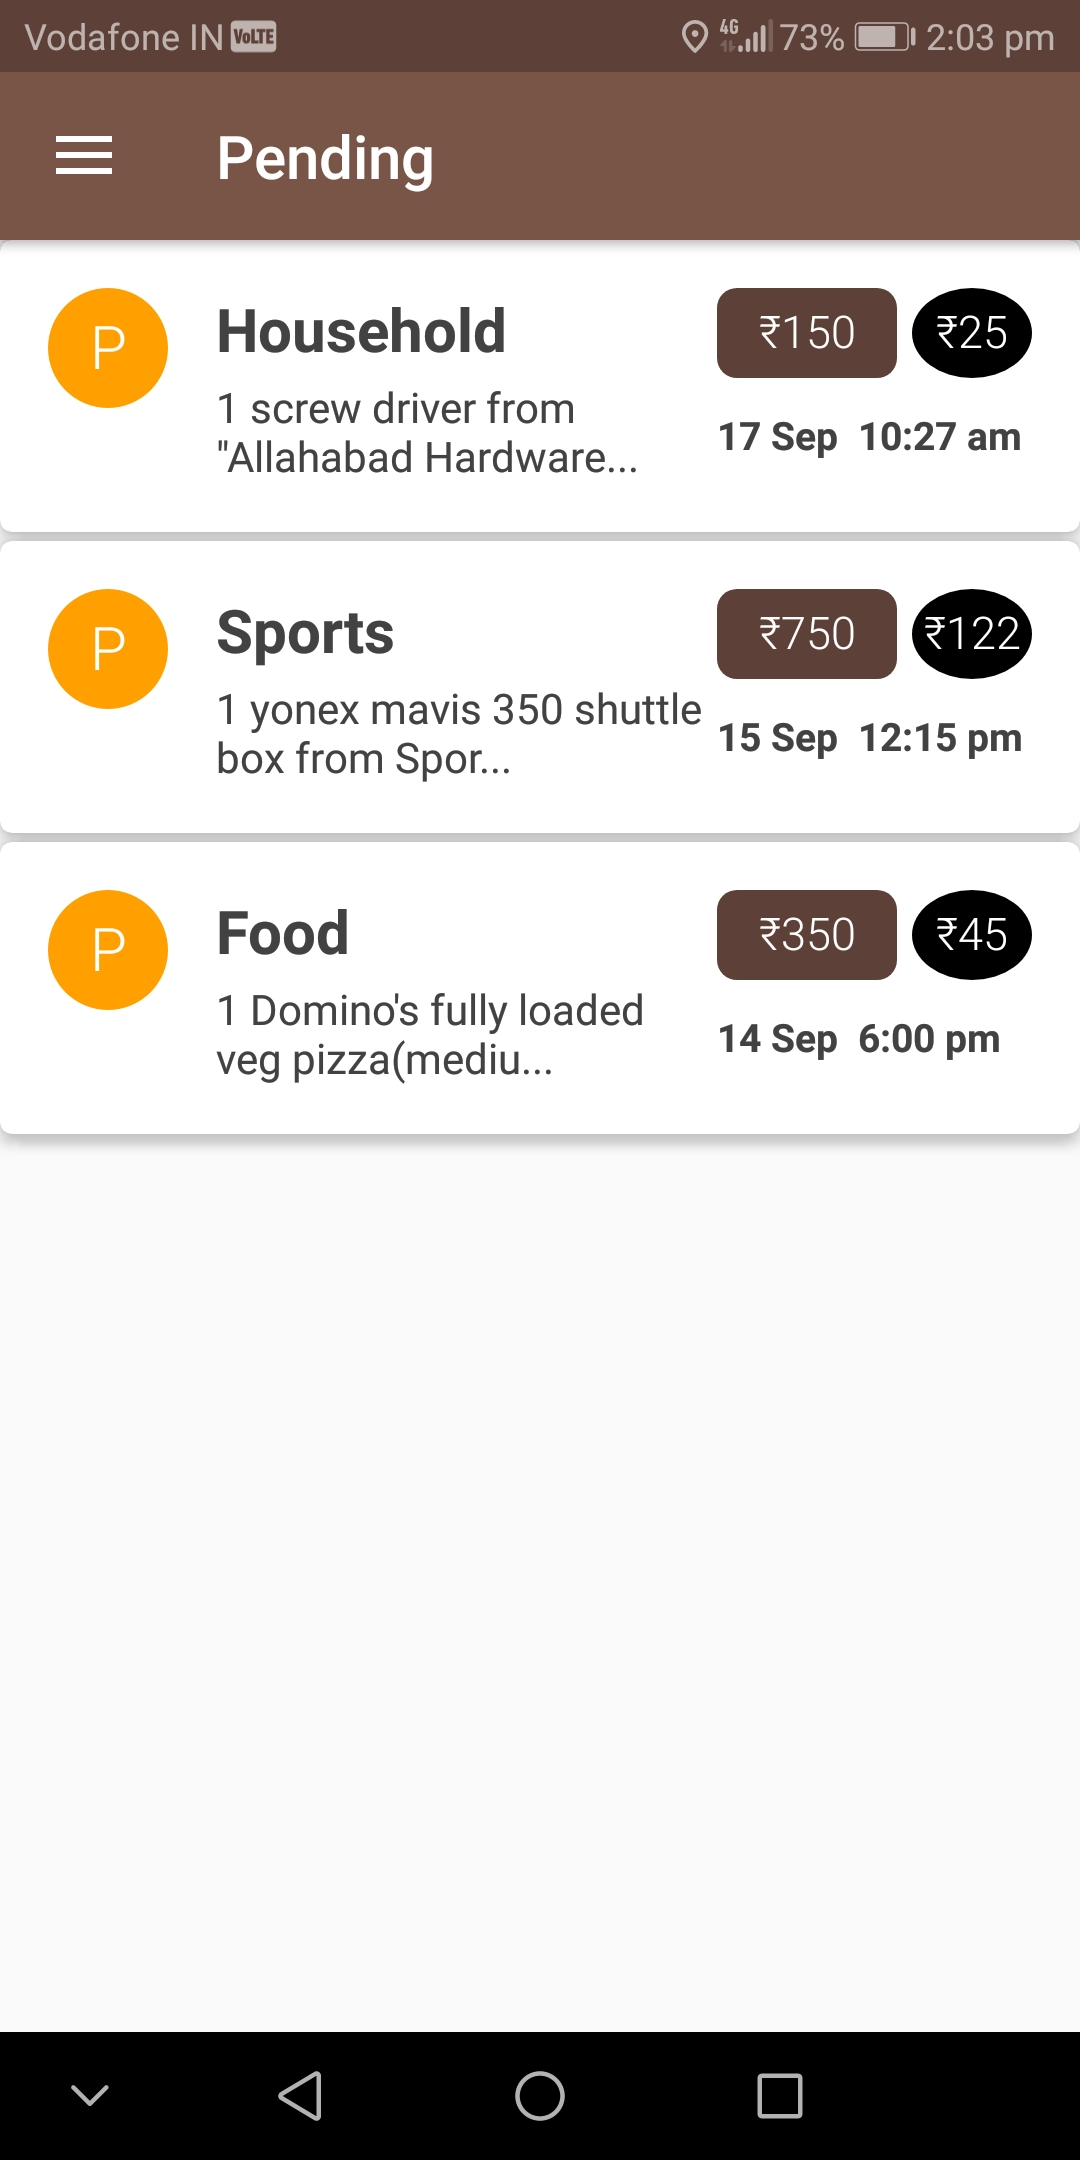
\includegraphics[width=4cm]{pending_orders.jpg}
\caption{\centering Pending orders}
\end{subfigure}
\begin{subfigure}[h!]{.24\textwidth}
\centering
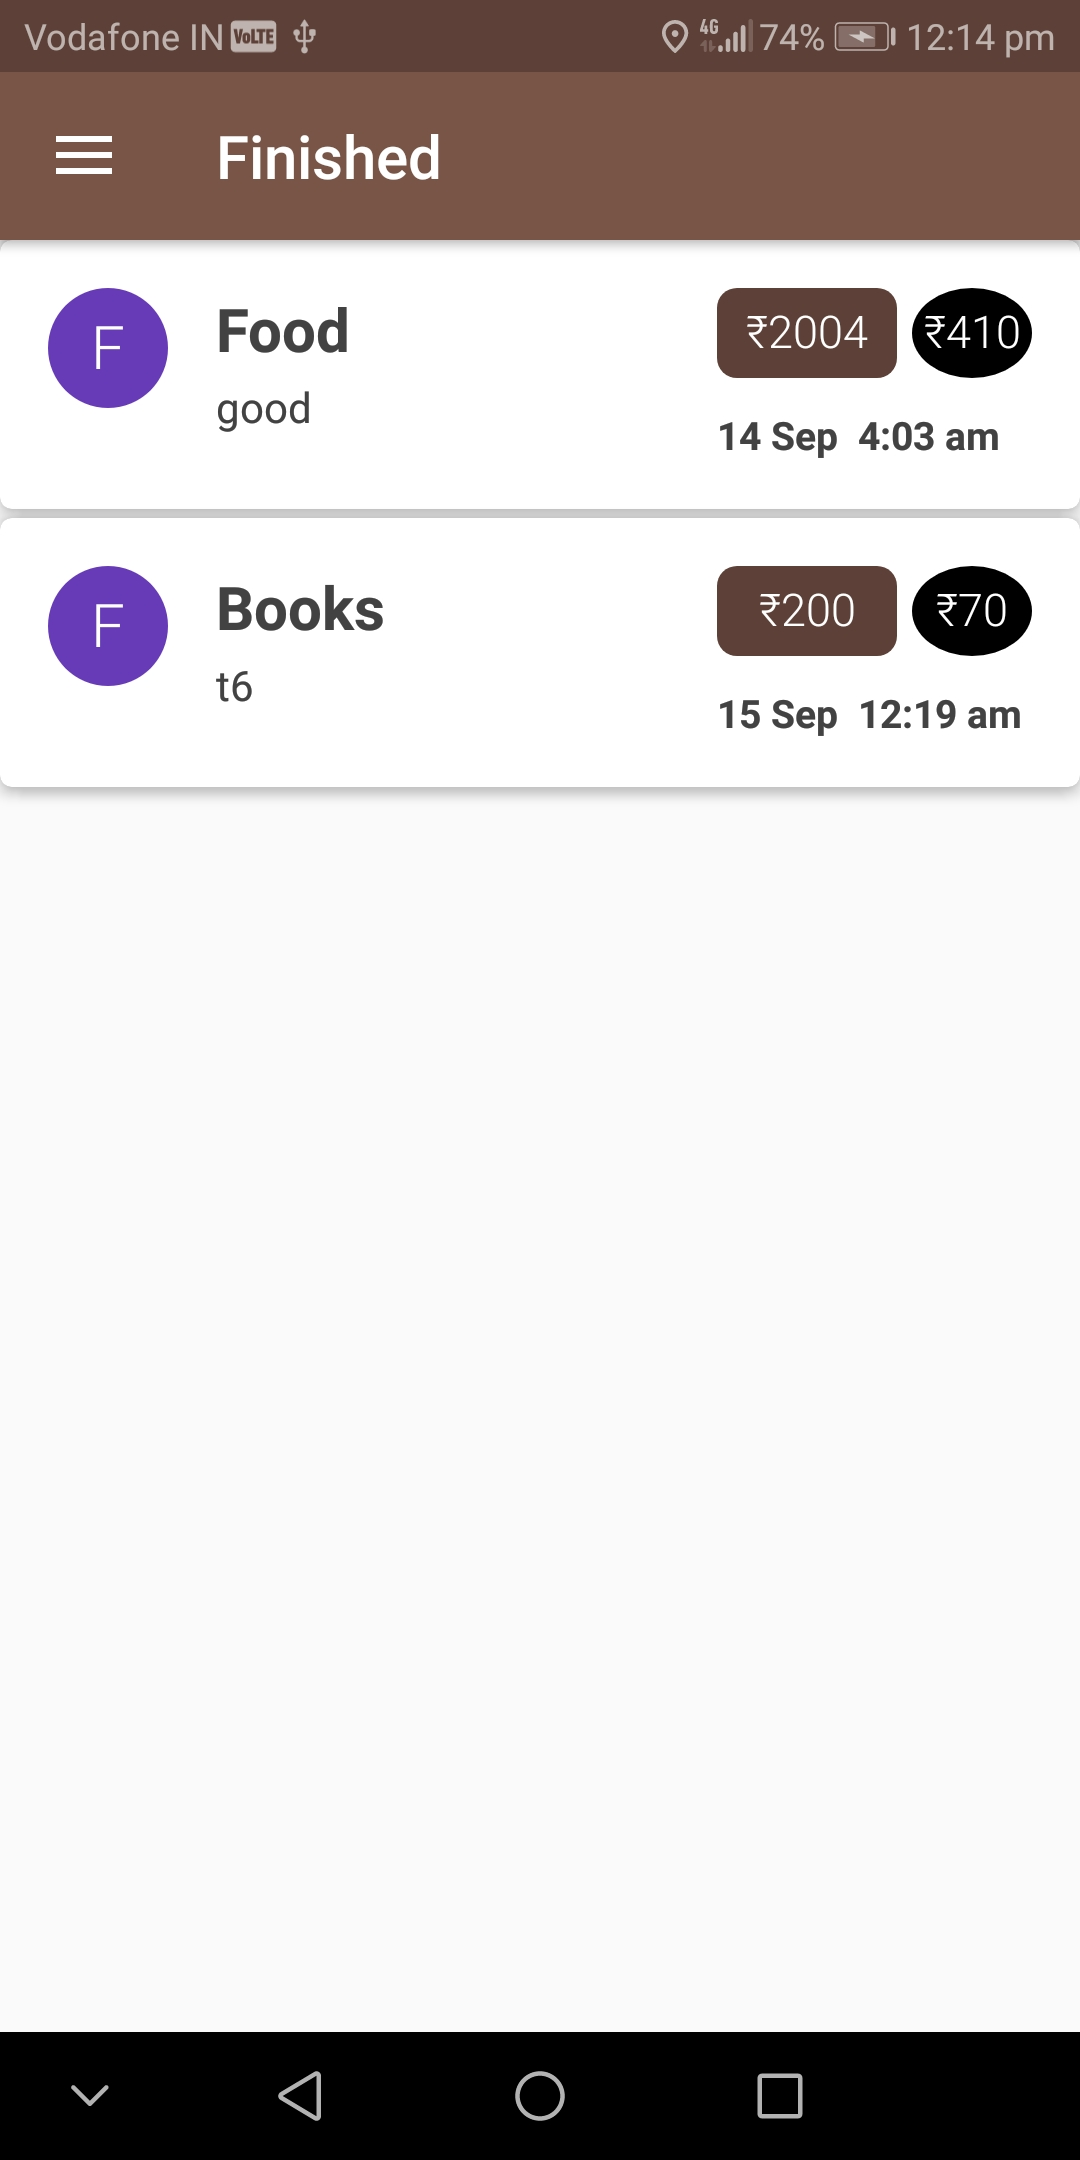
\includegraphics[width=4cm]{finished_deliverer.jpg}
\caption{\centering Finished orders}
\end{subfigure}
\caption{ Deliverer view} 
\label{fig:NASA_Logo}
\end{figure}


\subsection{Deliverer Order Detail View}
\begin{itemize}
\item It is similar to the Detailed order view of Shopper but according to a deliverer.
\item There is a SHOW PATH button which shows the path from your current location to the delivery location of that order.
\item When the order is pending, there is an ACCEPT button.
\item When the order is ACCEPTED, there is a button to reject as well as a button to COMPLETE ORDER.
\end{itemize}

\subsection{Accept an Order}
\begin{itemize}
\item A deliverer can Accept a pending order by touching the ACCEPT button in the detailed view of that order.
\end{itemize}

\begin{figure}[h!]
\begin{subfigure}[h!]{.24\textwidth}
\centering
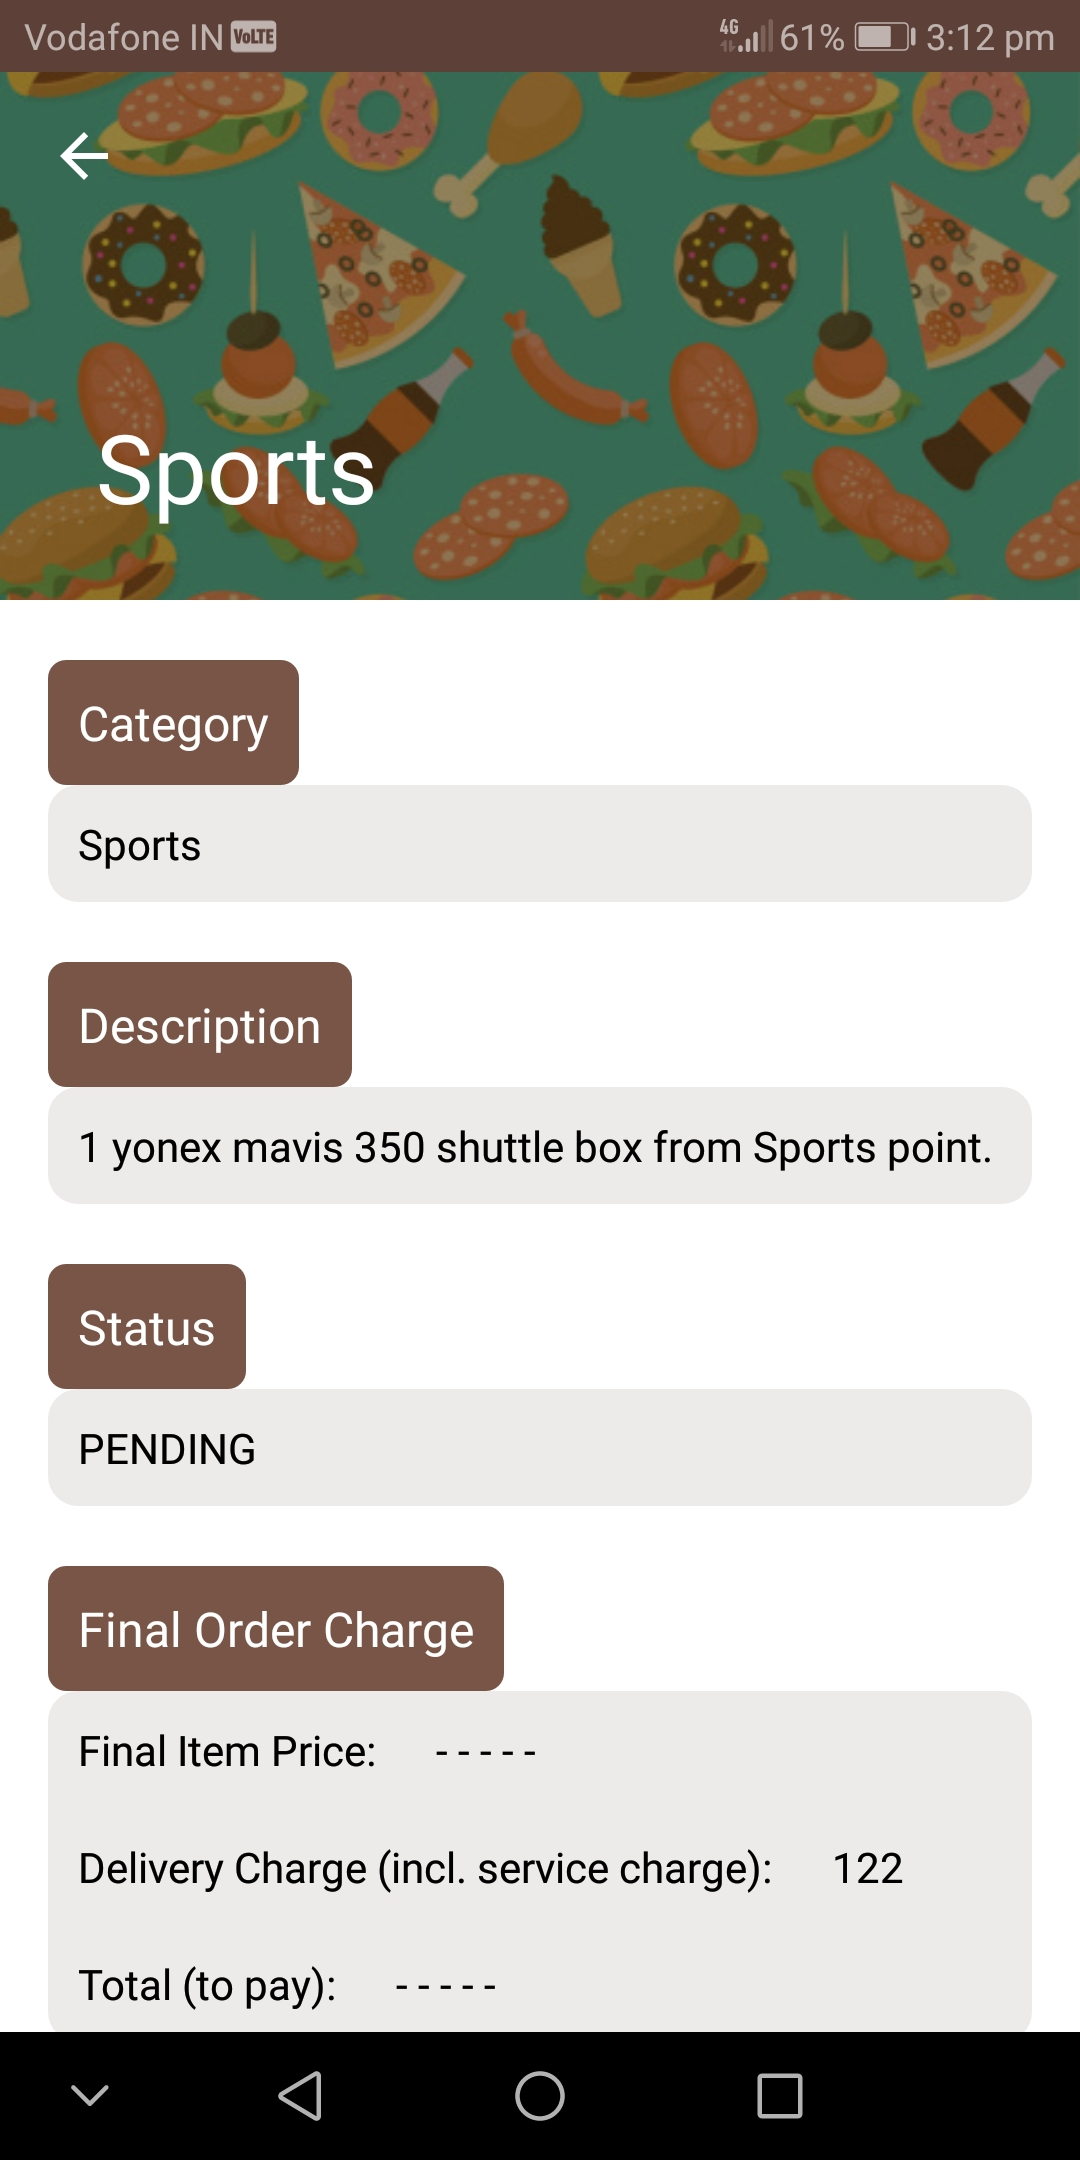
\includegraphics[width=4cm]{deliverer_order_detail1.jpg}
\caption{\centering Deliverer Order detail view}
\end{subfigure}
\begin{subfigure}[h!]{.24\textwidth}
\centering
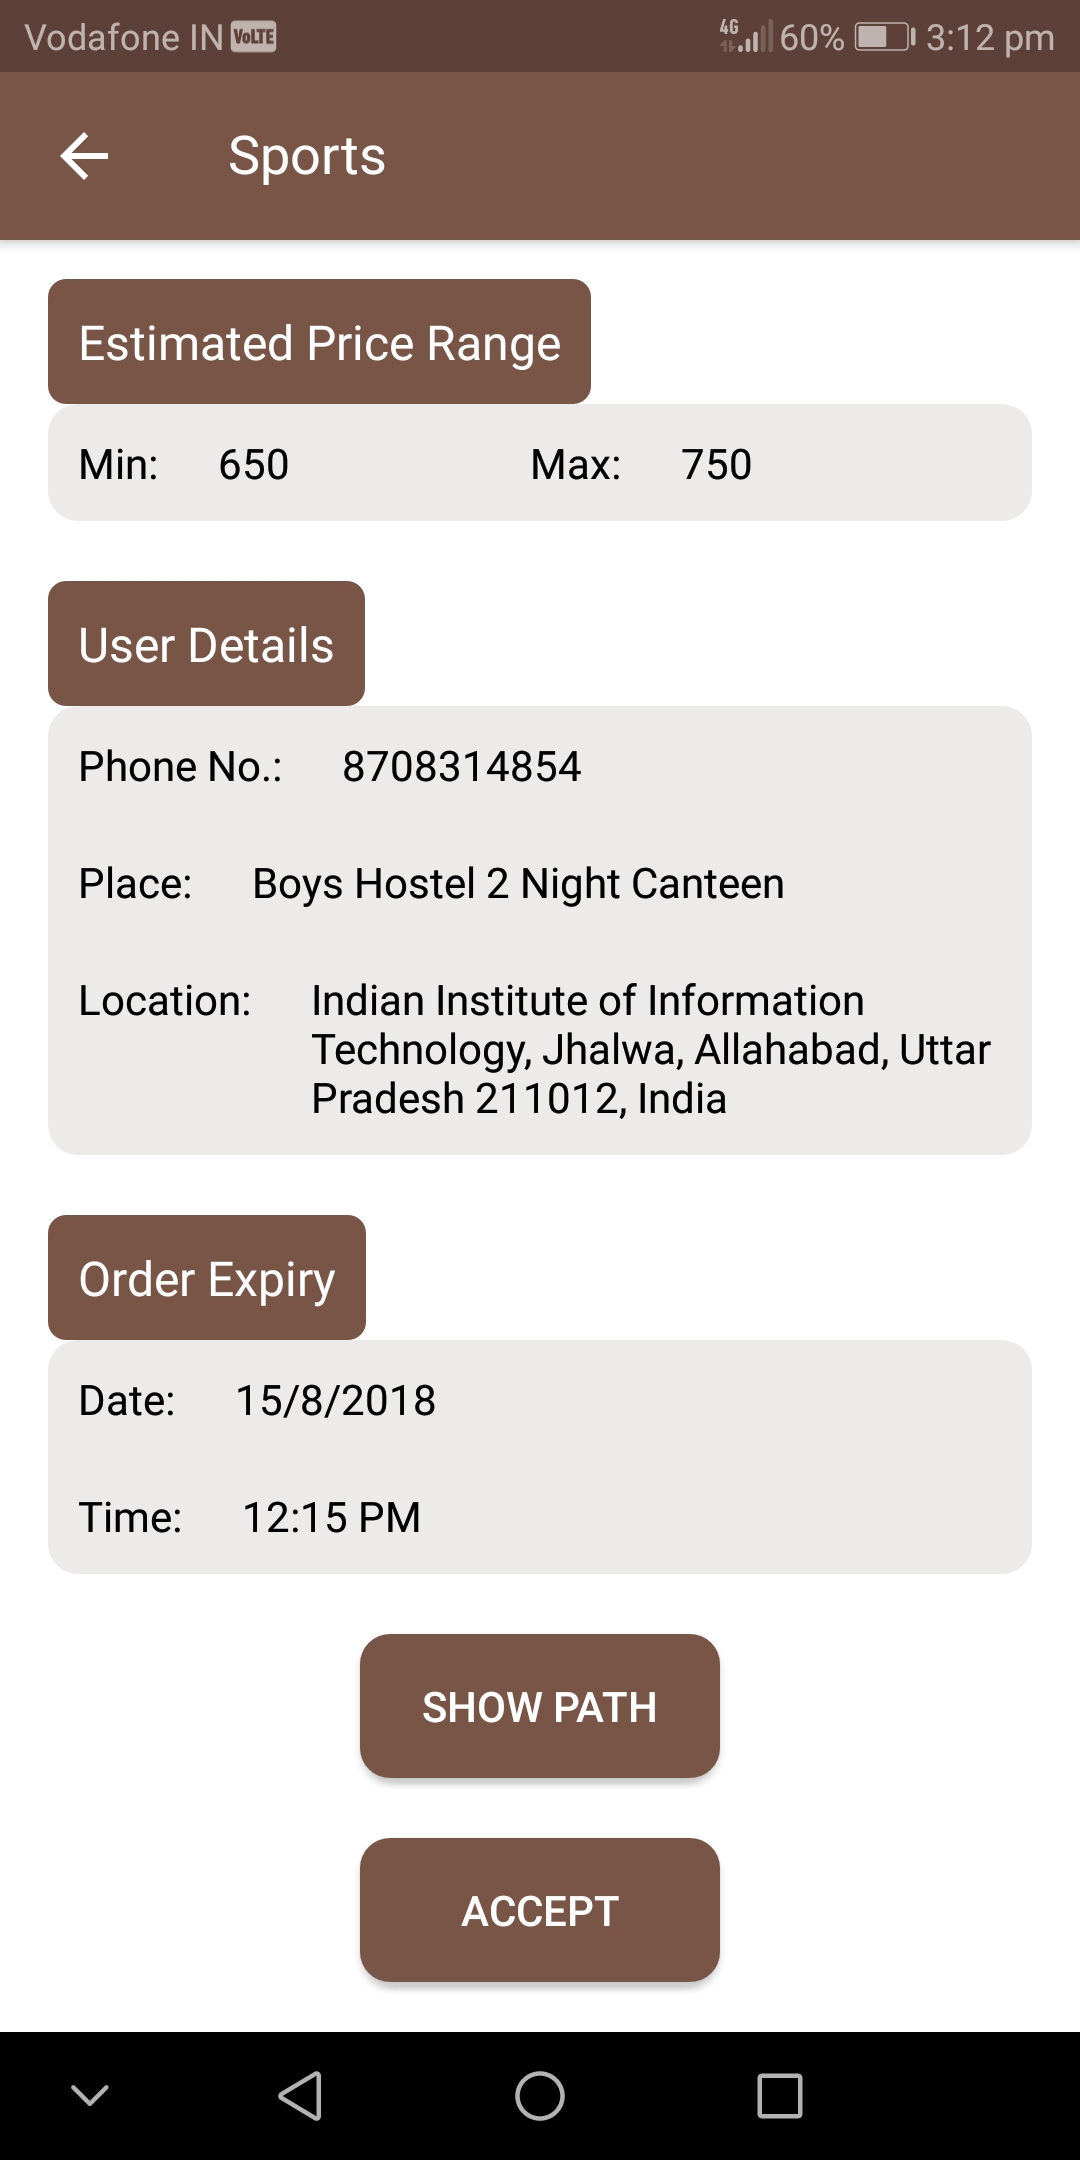
\includegraphics[width=4cm]{deliverer_order_detail2.jpg}
\caption{\centering Deliverer Order detail view}
\end{subfigure}
\begin{subfigure}[h!]{.24\textwidth}
\centering
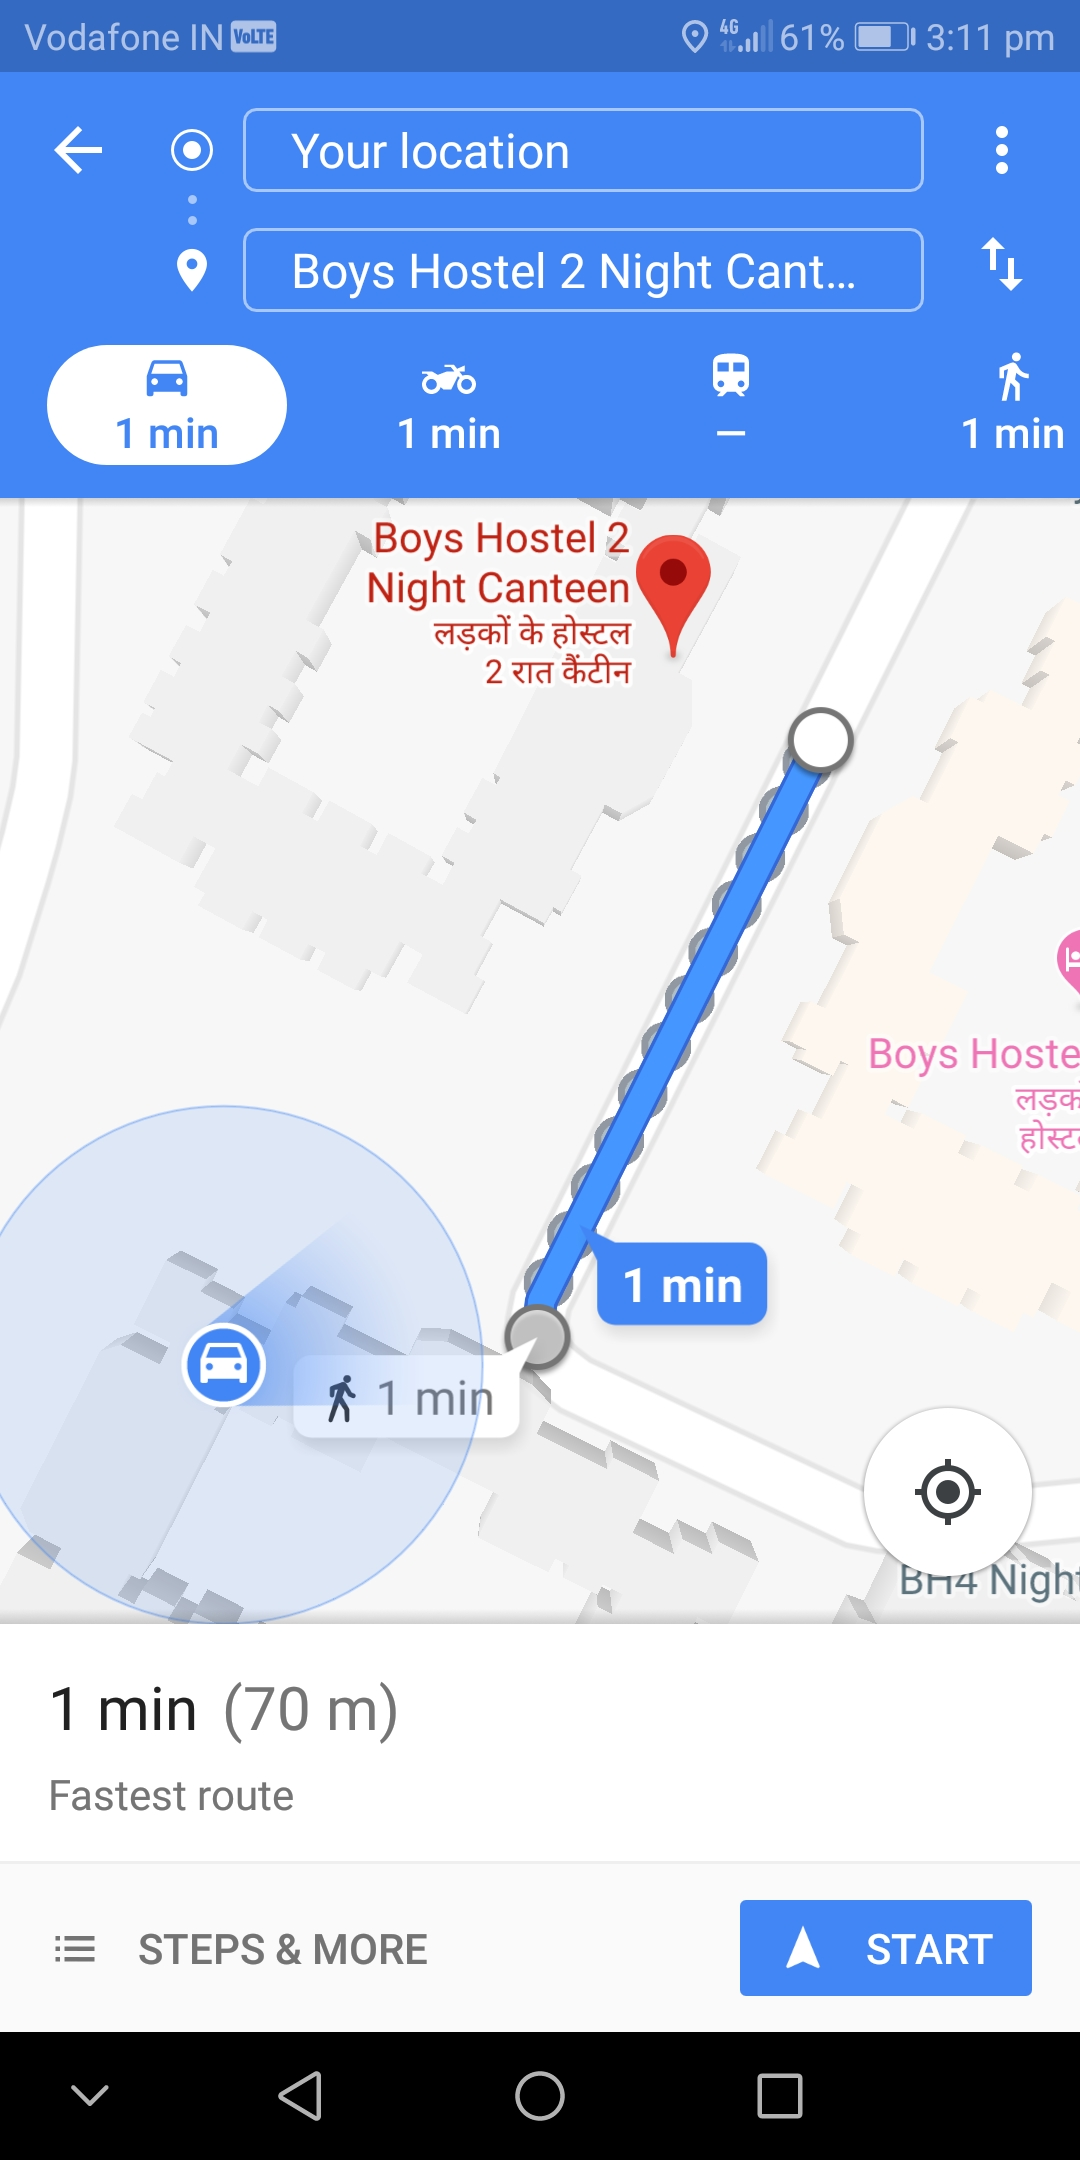
\includegraphics[width=4cm]{show_path.jpg}
\caption{\centering Show Path functionality using Google Maps}
\end{subfigure}
\begin{subfigure}[h!]{.24\textwidth}
\centering
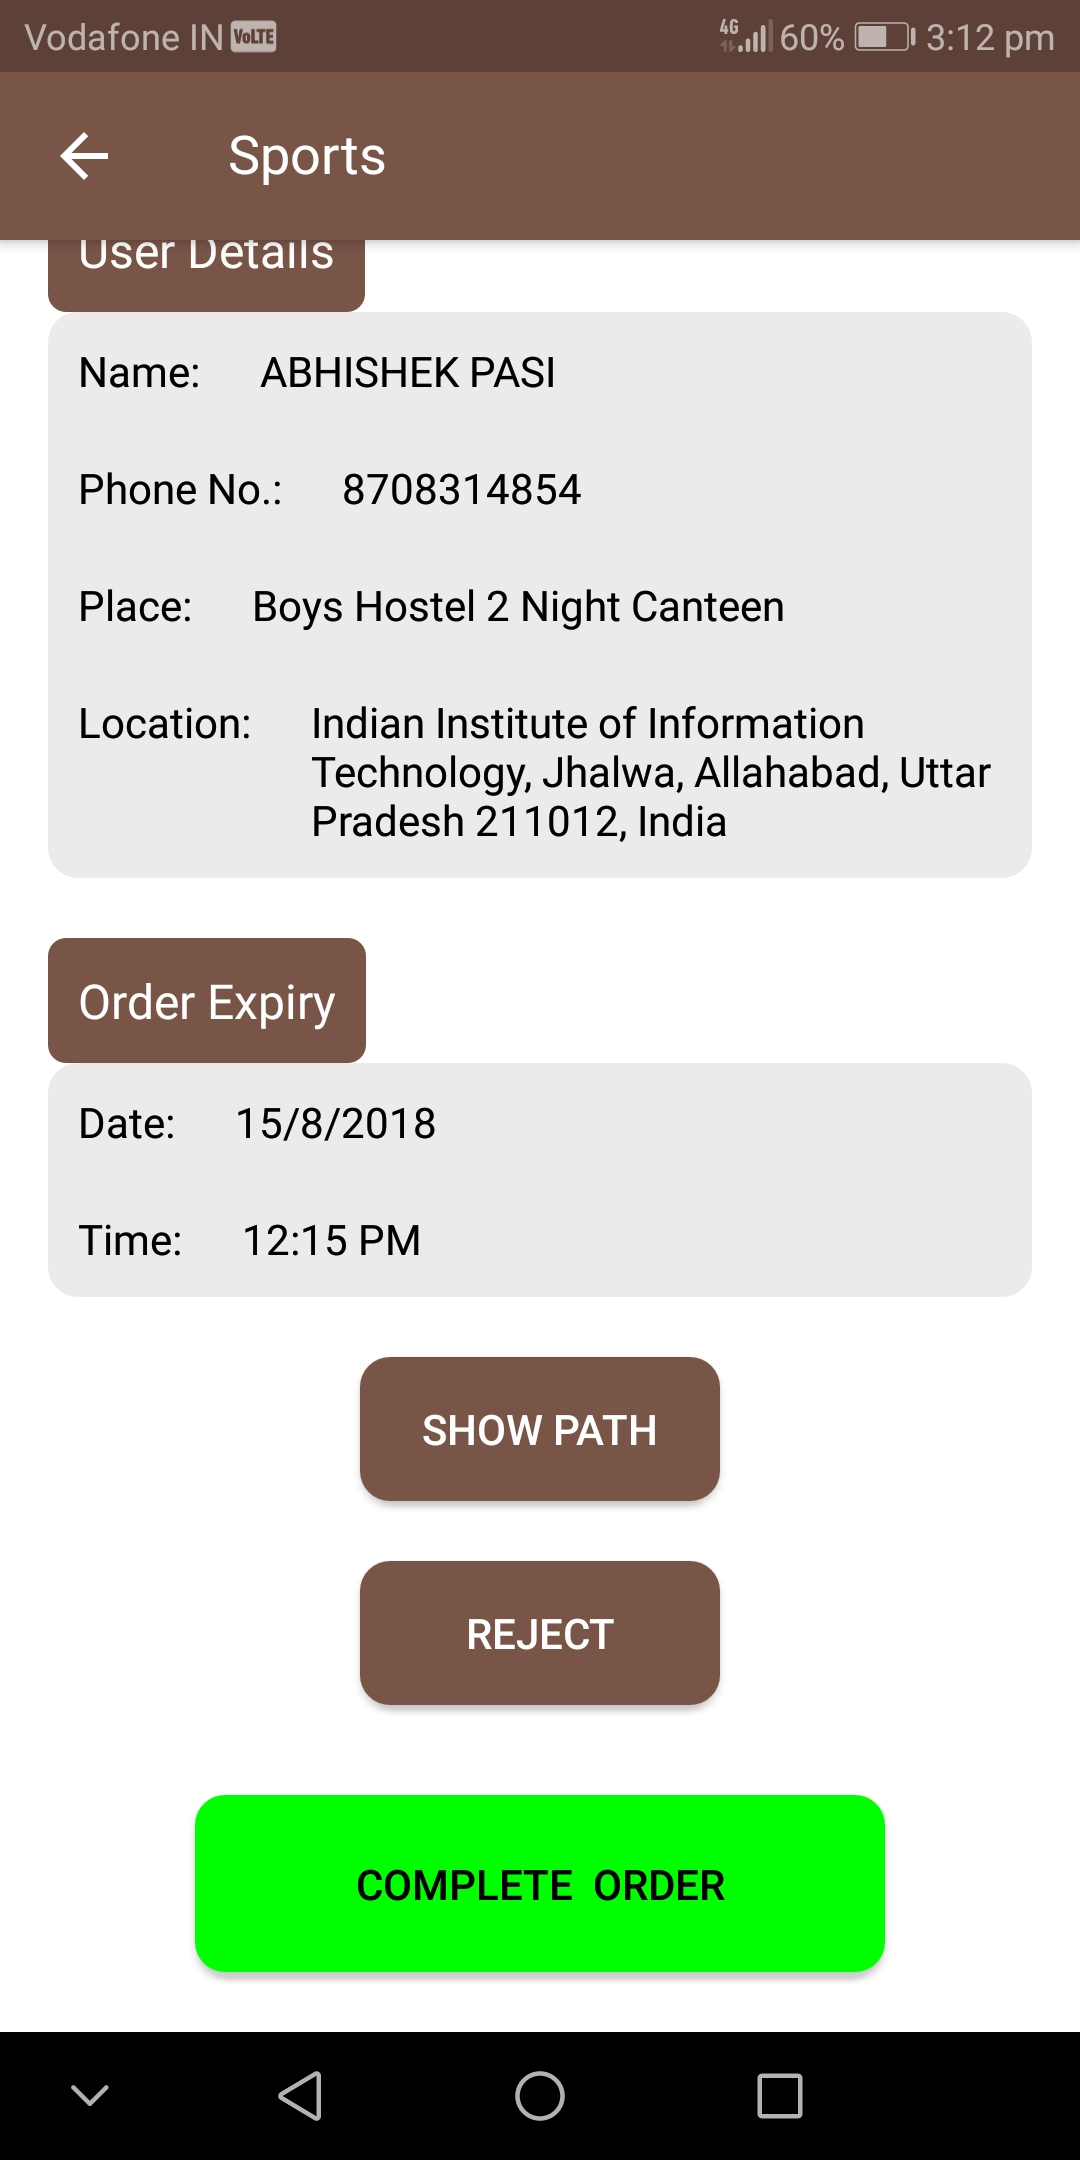
\includegraphics[width=4cm]{order_accepted.jpg}
\caption{\centering Accepting an order by touching the Accept button}
\end{subfigure}
\caption{Accepting an order} 
\label{fig:NASA_Logo}
\end{figure}


\subsection{Complete Order}
\begin{itemize}
\item By touching the COMPLETE ORDER button, we start the process of completing the order.
\item First a screen is displayed which asks the deliverer to enter the Actual price paid to buy the order, after filling the price, the SEND OTP button is activated, using which an OTP along with the price as filled by the deliverer is sent to the respective shopper of that order in the form  of a notification.
\item Then, a new screen is displayed to the deliverer, asking to enter the OTP as received from the shopper.
\item The OTP is working as a confirmation from the shopper. So, a shopper will give the OTP to the deliverer only when he/she is satisfied with the price and quality of the delivery.
\item After entering the correct OTP by the deliverer, the delivery of that order is considered to be finished.
\end{itemize}

\begin{figure}[h!]
\begin{subfigure}[h!]{.3\textwidth}
\centering
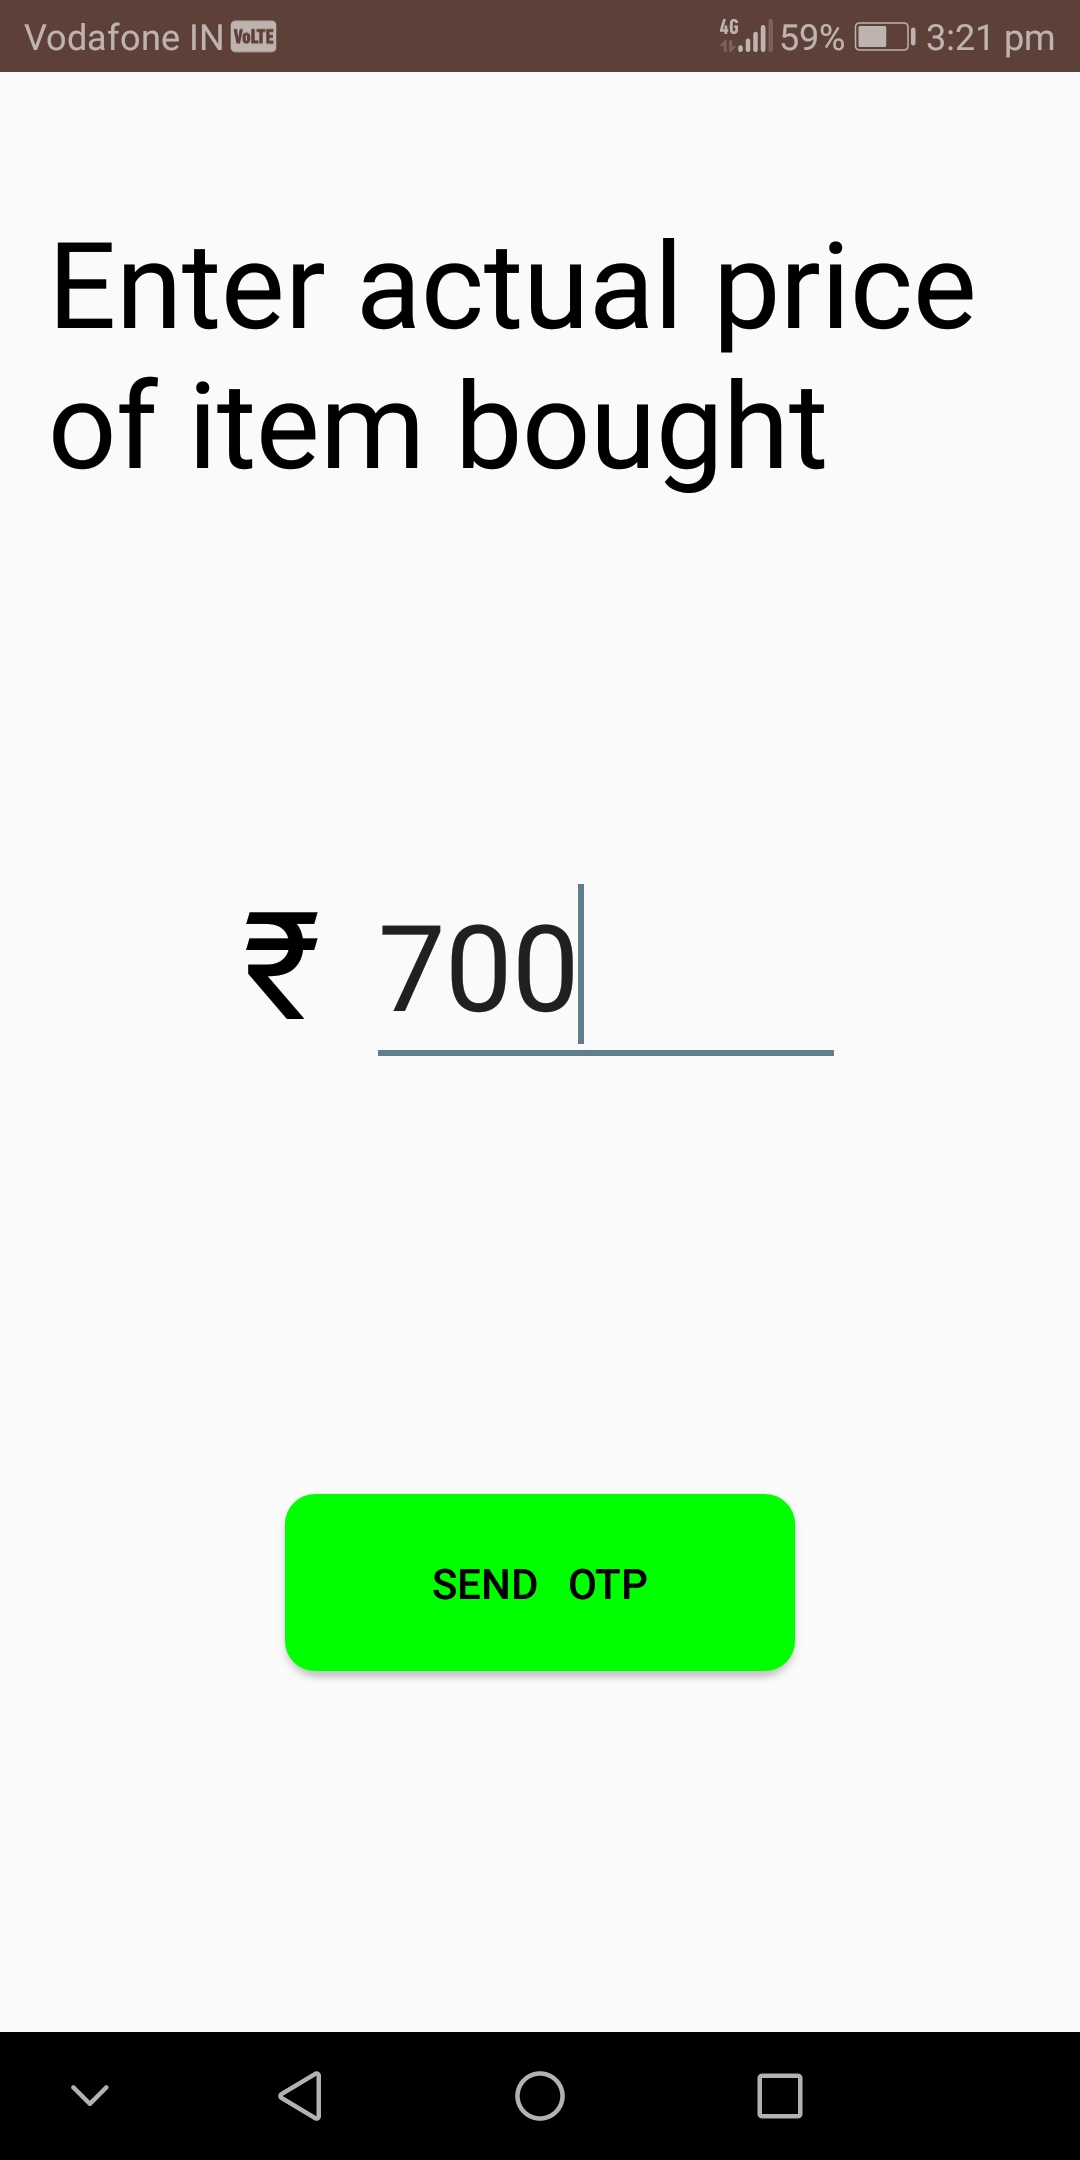
\includegraphics[width=5cm]{send_otp.jpg}
\caption{\centering Sending OTP to Shopper after entering the Actual price of order}
\end{subfigure}
\begin{subfigure}[h!]{.3\textwidth}
\centering
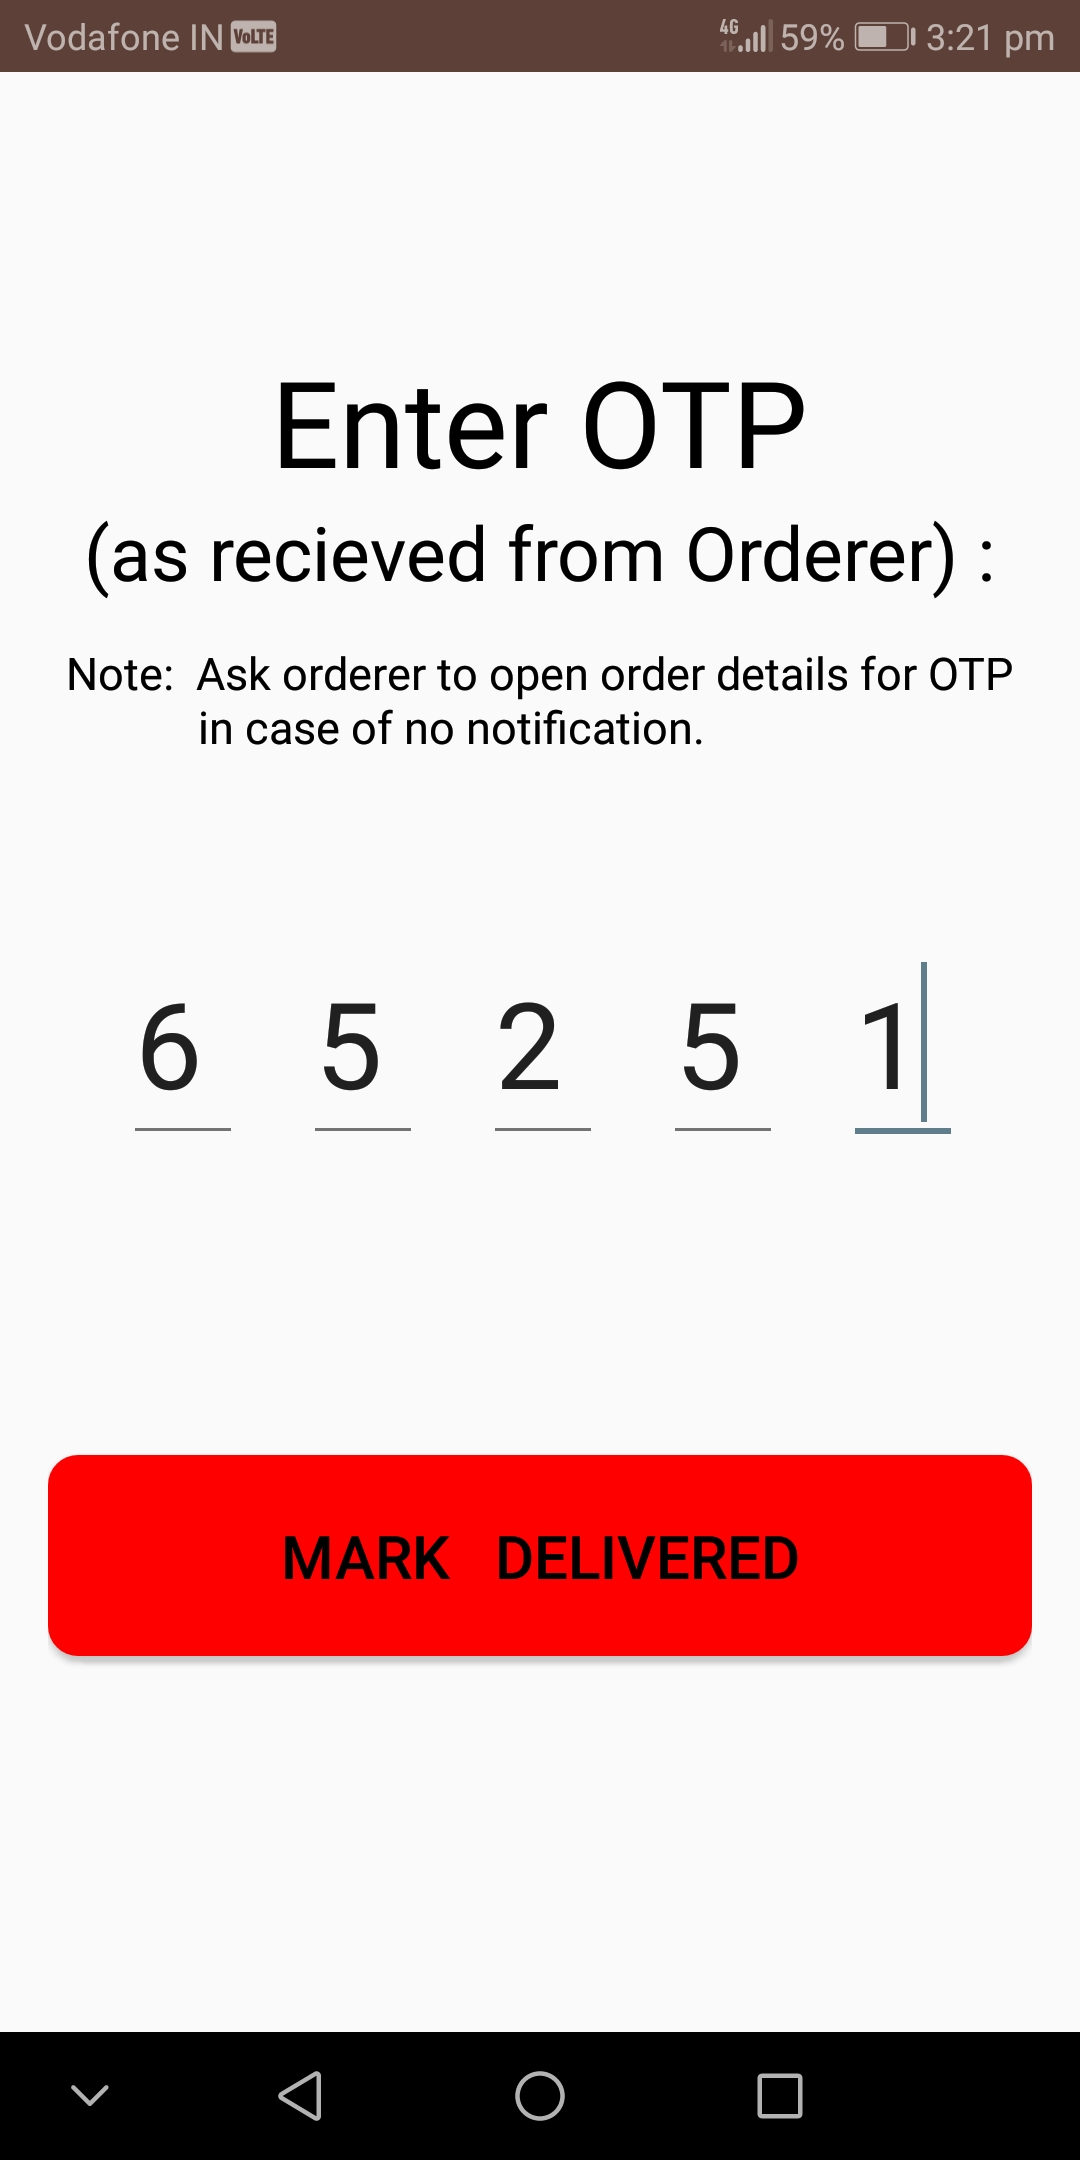
\includegraphics[width=5cm]{mark_delivered.jpg}
\caption{\centering Entering the OTP as received from Shopper to finish Delivery}
\end{subfigure}
\begin{subfigure}[h!]{.3\textwidth}
\centering
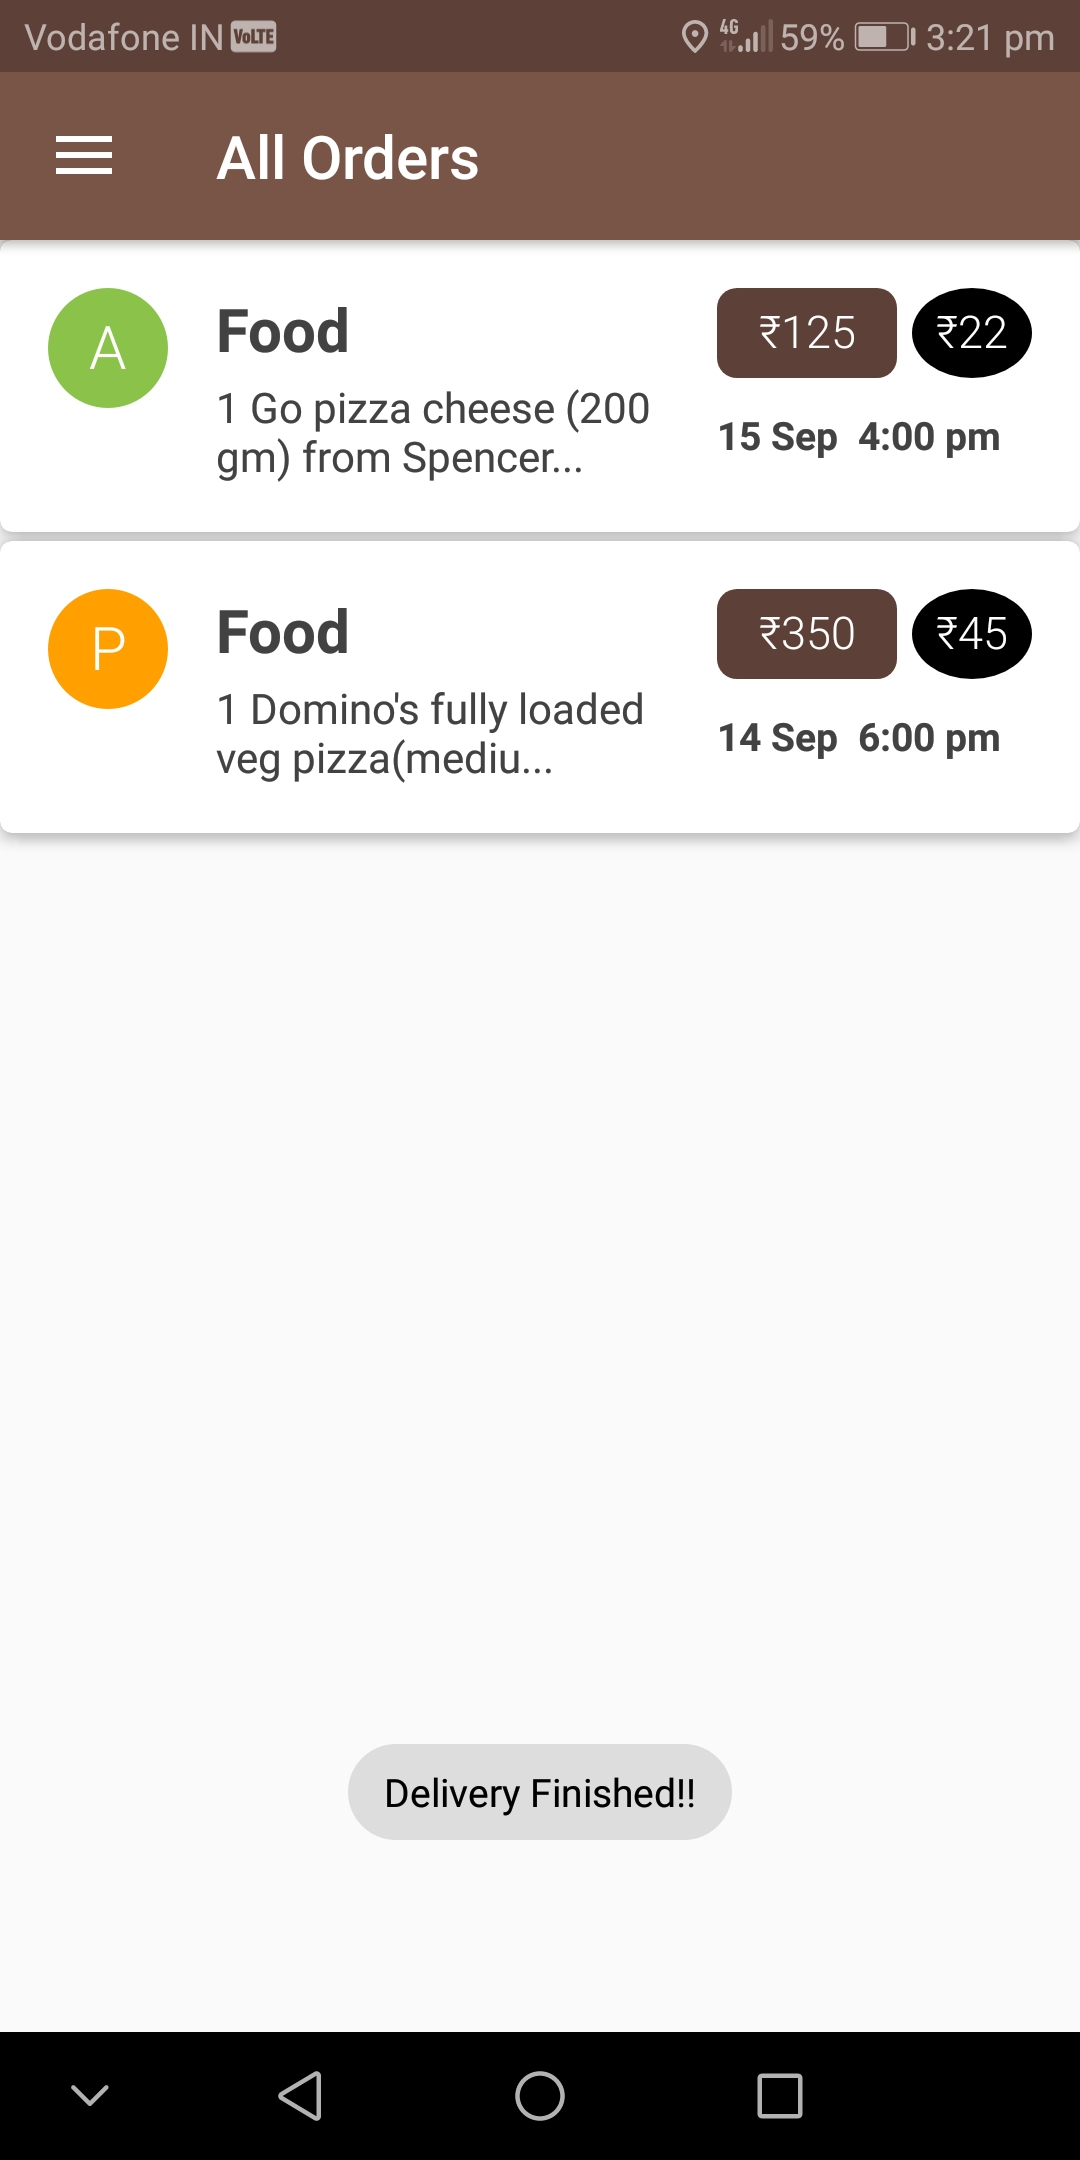
\includegraphics[width=5cm]{delivery_finished.jpg}
\caption{\centering Message confirming the Finishing of Delivery of order}
\end{subfigure}
\caption{Completing the Delivery of an order} 
\label{fig:NASA_Logo}
\end{figure}

%----------------------------------------------------------------

\chapter{Technology used}
\bigskip
\bigskip
\begin{itemize}[label=$\diamond$]
\item Softwares :
\begin{itemize}[label=$\rightarrow$]
\item Android Studio : Development environment for Google\textquotesingle s Android operating system.
\end{itemize}
\item Languages :
\begin{itemize}[label=$\rightarrow$]
\item For Front-end : XML(eXtensible Markup Language) and Android(Java)
\item For Back-end : Java
\end{itemize}

\item Tools / Libraries:
\begin{itemize}[label=$\rightarrow$]
\item Google Sign-in
\item E-mail verification (using Firebase Authentication)
\item Google Places API
\item Google Maps
\item Location
\item PayTM payments SDK
\item OneSignal API (for Notifications)
\item Lucidchart.com (for diagrams)
\end{itemize}

\item Databases :
\begin{itemize}[label=$\rightarrow$]
\item Google Firebase (NoSQL Real-time cloud-hosted Database) :
\begin{enumerate}
\item Data is synced across all clients in realtime, and remains available when your app goes offline.
\item Data is stored as JSON (JavaScript Object Notation) tree.
\end{enumerate}
\end{itemize}

\end{itemize}



%---------------------------------------------
\chapter{Business Model}
\bigskip
\bigskip
\bigskip
 Our application can be used as a Business application or it can be used among friends for their logistic and shopping  needs.\\

As a business plan we are charging shoppers some delivery charge for the service we provide. The deliverer gets some incentive for delivering the order.\\

The delivery charge can be shared between us and the delivery person. When we find less deliverers are willing to use our app, we may increase their incentive to make up for the number of deliverers. \\

Also, we initially planned to launch this app in our college. We didn\textquotesingle t do so due to time constraints and some other reasons.\\

For more smooth functioning of our application we may collaborate with third party delivery services.\\

We will discuss more business opportunities in future work section of our report.\\


\chapter{Current status of Project}
\bigskip
\bigskip
\bigskip
\bigskip

Currently all the basic features mentioned in this report are working properly.\\

We have tested our application for various scenarios like
\begin{enumerate}[label=\roman*)]
\item  if network is not working properly we are not allowing any action such as accept or reject as it may lead to confusion between users.
\item we are asking for location so that one can only accept same city orders.
\item  Updating the user screen as soon as status of any of the order changes to avoid ambiguity that may arise if a user cancels an active order.
\item Since our app is quite realtime (order status might change anytime) , we have taken care of any of the corner cases that may cause conflicts in status of orders. However , it may happen that some cases did not cross our mind, you may suggest if you find any of those. We will fix issues as soon as we find them.

\par We don\textquotesingle t have access to all the features that PayTm gateway provides . Since we have testing credentials for the gateway , we can only simulate the process of making of payment currently  . However, the gateway is fully functional .
To get a genuine merchant id , we need to register a company name.

\end{enumerate}


\chapter{Future scope}
\bigskip
\bigskip
\bigskip
\bigskip

While discussing Use case section of Software requirement Specification (SRS) of our project , we told about some use cases which can be thought of .
We may modify our application to suit specific needs.\\

Example of few such use cases :-
\begin{enumerate}[label=(\roman*.)]
\item Partnering with local shops and having centralised system of delivery between the shop and its customers. 
\item Having listing of shops and using the application to buy goods from shops.
\item Partnering with restaurants for booking tables or ordering food items from their menu.

\end{enumerate}

\chapter{How to use our App}
Here we present a simple and summarised way on how to use our app.
Our app has two modes of usage namely Shopper and Deliverer and corresponding two main functionalities namely Place an order and Deliver an order.
    Below we give summarised steps on how to execute these two main functionalities.

\section{Place an order}
\begin{itemize}[label=$\rightarrow$]
\item Choose Shopper mode.
\item Click on the floating action button (`+').
\item Fill all the details.
\item Add location from the map. (uses google place picker\cite{c14} api).
\item Add expiry date and expiry time\footnotemark.
\item Click proceed button after you have completed.
\item A bottom sheet appears which calculates and shows delivery charge.
\item After that you need to pay for the order using Paytm wallet\footnotemark.
\item You will be prompted to login into Paytm. (Don\textquotesingle t login into you real Paytm account instead use test credentials provided by us).
\begin{description}
\item Mobile No. \quad -- \quad7777777777
\item OTP \quad \quad \quad \quad-- \quad489871\\
\item Few things to note :-
\begin{itemize}[label=$\diamond$]
\item You can left swipe to cancel this order.
\item You can undo the cancel operations within 3 seconds.
\end{itemize}
\end{description}
\item When payment is complete you will be redirected back to User Screen.
\item You can see your order on the screen.
\end{itemize}

\footnotetext[1]{You order expires as soon as clock hits the expiry time and date. No deliverer will be able to see an expired order.}
\footnotetext[2]{Right now we are in sandbox mode, we have a demo merchant id.}

\subsection{Circle Notation :}
\begin{itemize}[label=$\circ$]
\item P - pending orders
\item A - active orders
\item F - Finished orders
\item C - Cancelled orders
\item E - Expired Orders 
\end{itemize}
These all type of orders can be accessed via filters in navigation bar.

\section{Deliver an order}
\begin{itemize}[label=$\rightarrow$]
\item Choose Deliverer mode.
\item You will see various pending orders on your screen.
\item Open the order you are interested to deliver.
\item Accept the order. (A notification goes to customer associated with that order)
\item You may also reject, if you change your mind. (Again, a notification goes to user)
\item A bright green button named COMPLETE ORDER appears on the order detail page of the order you accepted.
\item After you purchase the item press the bright green COMPLETE ORDER button.
\item You will be asked to enter actual price of item you bought (excluding delivery charges).
\item You press a send OTP button.
\item Enter the OTP provided by user to finish the order.

\end{itemize}
%---------------------------------------------------------------------------------------------------

\chapter{About Database}

\begin{itemize}
\item We are using Google Firebase Database which is a NoSQL Real-time cloud-hosted Database.
\item As our app is quite real-time (order status might change anytime) we needed the properties of a real-time database.
\item Real-time syncing makes it easy for our users to access their data from any device. Real-time Database also helps your users collaborate with one another as data is synced across all clients in real-time, and remains available when our app goes offline.
\item All the database queries like reading and writing data are fully asynchronous. This means that the call always returns immediately, without blocking the code to wait for a result. The results come some time later, whenever they’re ready, this results in overall faster response time for our app. Also asynchronous tasks run on parallel threads which make use of multiprocessing power of our device.
\item If queries were synchronous , it will hold on the app till the result is obtained . This may lead to crashes and freezes in user interface .   
\end{itemize}

\section{NoSQL v.s SQL database}
\begin{itemize}
\item NoSQL databases were created to overcome the limitations of relational database technology.
\item NoSQL databases are more flexible, scalable and also superior in the performance when compared to relational databases.
\item NoSQL helps to store information without doing up‐front schema design.
\item NoSQL data model has fewer restrictions and easily allow new changes without creating much fuss.
\item NoSQL is cost effective compared to RDBMS and allows to process and store more data at a much lower cost because RDBMS rely on overpriced storage and proprietary server systems while NoSQL databases commonly rely on clusters of cheap commodity servers.
\end{itemize}

\section{Cloud-hosted vs Local server}
\begin{itemize}
\item The application will run 24x7 if internet connection is available.
\item Data is synced across all clients in real time, and remains available when our app goes offline.
\item As we are using third-party (Google Firebase) as our cloud hosting provider, we do not need to worry about security and  where the data is stored. 
\item Whereas in local server we would have to maintain it fully and ensure that the server is available 24x7.
\end{itemize}


\section{Database Structure}
All the data is stored as JSON (JavaScript Object Notation) tree.
\begin{itemize}
\item JSON is preferred over XML as the primary data format for transmitting back data, because it is much more lightweight.
\item It is easy for humans to read and write. 
\item It is easy for machines to parse and generate.
\item It is a text format that is completely language independent.\\
\end{itemize}

JSON is built on two universal data structures:
\begin{itemize}
\item A collection of name/value pairs. In various languages, this is realized as an object, record, struct, dictionary, hash table, keyed list, or associative array.
\item An ordered list of values. In most languages, this is realized as an array, vector, list, or sequence\cite{c1}.
\end{itemize}


\begin{figure}[h!]
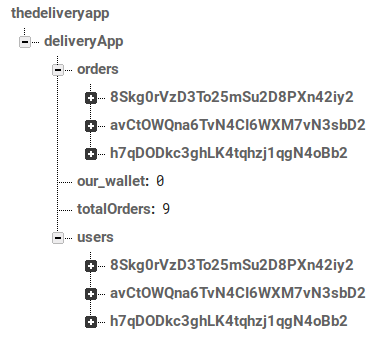
\includegraphics[width=14cm]{overall_tree.png}
\caption{Our database JSON tree}
\label{fig:NASA_Logo}
\end{figure}

\begin{figure}[h!]
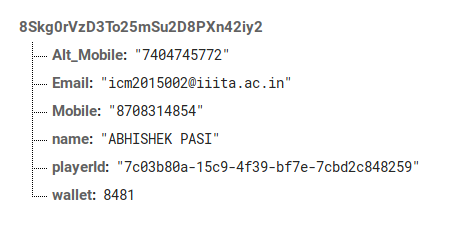
\includegraphics[width=16cm]{user.png}
\caption{Structure of a user in our database}
\label{fig:NASA_Logo}
\end{figure}

\begin{figure}[h!]
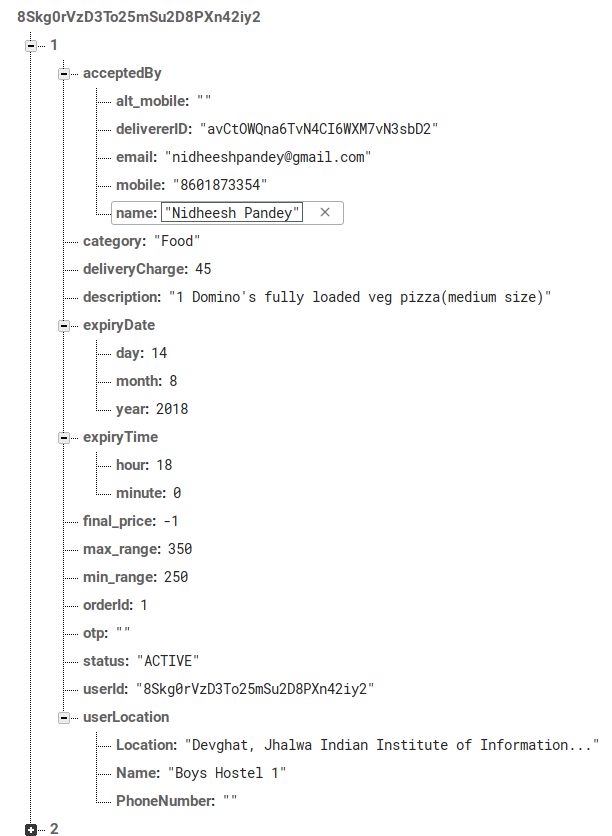
\includegraphics[width=18cm]{order.png}
\caption{Structure of an order in our database}
\label{fig:NASA_Logo}
\end{figure}


%---------------------------------------------------------------------------------------------------


\bibliographystyle{IEEEtran}
\bibliography{./references}
\end{document}